\documentclass{seal_thesis}

\thesisType{Master's Thesis}
\date{\today}
\title{CLI-Tutor}
\subtitle{Can interactive learning make the command line more approachable?}
\author{Qasim Warraich}
\home{Lahore} % Geburtsort
\country{Pakistan}
\legi{18-787-796}
\prof{Prof. Dr. Harald C. Gall}
\assistent{Dr. Carol V. Alexandru-Funakoshi}
\email{qasim.warraich@uzh.ch}
\turl{gitlab.com/qasimwarraich/cli-tutor}
\begindate{2022-03-14}
\enddate{2022-09-14}

%% OUTLINE
% - Abstract
% - Overview
%   - problem description
%       - potential solution
%   - introduce tool
%   - outline thesis
% - Introduction
%   - Interactive learning tools
%   - Requirements
%       - RQs
% - Tool (CLI-Tutor)
%   - overview
%       - cirriculum
%       - lesson design
%       - usability considerations
%            - deliberate emphasis on easy vocabulary
%       - safety considerations
%   - web version
% - Design and Implementation
%   - overview
%   - original tinkering and considerations
%   - features and considerations
%       - readline
%       - golang
%       - logging
%           - remote phoning home
%       - extensibility (markdown, parser)
%       - embedded files
%           - Template expansion
%           - Running examples
%       - usability 
%   - architecture of cli-tool
%   - architecture of web-tool
%       - how sandboxing is achieved
% - User Study
%    - methodology
%       - assignment
%       - survey structure
%    - participants
% - Results
%    - the cli-tutor tool (result of engineering work)
%       - future work
%    - user study
%       - analysis
%       - user study
% - Related Work and Reflections (possibly seperate)
%   - related work
%   - future work
%       - improvements to CLI-Tutor
%       - areas to explore in the space
% - Conclusion
% - Appendix
%   - Survey questions
%   - Detailed dev considerations

\begin{document}
\maketitle

\frontmatter

% acknowledgements

\begin{acknowledgements}
I would like to acknowledge my Thesis advisor Dr. Carol V. Alexandru-Funakoshi
for his support and encouragement throughout this thesis work.

Additionall I would like to thank....

\end{acknowledgements}


% abstract(s)
\begin{abstract}

Despite the arguably dated appearance, difficult learning curve and practical
non-existence in the general personal computing space, Command Line Interfaces
(CLIs) have more than stood the test of time in the software development world.
There are a multitude of extremely popular tools and applications that
primarily focus on the command line as an interaction medium. Some examples
include version control software like git\footnote{git source code version
control tool: \href{https://git-scm.com/}{https://git-scm.com/} }, compilers and
interpreters for programming languages, package managers and various core
utilities that are popular in areas such as software development, scripting and
system administration.

As mentioned before, the use of the command line as an interaction paradigm has
effectively disappeared from a mainstream personal computer usage perspective.
This contributes greatly to the intimidation factor and learning difficulty for
those interested in getting into software engineering or system administration.
This unfamiliarity, paired with the inevitability of usage of CLIs in the
development space highlights a need to make the command line more accessible to
new users for whom text-based interaction with their computer is an alien
concept. In recent years interactive learning utilising tools such as sandboxed
environments have been gaining in popularity and have the potential to be a
suitable medium for learning command line basics through actual usage, examples
and practice.

\end{abstract}


\tableofcontents
\listoffigures
\listoftables
\lstlistoflistings

\mainmatter

%TODO MAKE SURE SCREENSHOTS REFLECT TYPO FIXES
%TODO SHOULD NUMBERS BE NUMBERS OR TEXT ?
%TODO ADD REFERENCES TO ALL TECHNOLOGIES
%TODO FINISH INTRO
%TODO:(extending section) Check if the "following page" thing holds true in the final version of the paper.

% TODO: Counter reset?
% \makeatletter
% \AtBeginDocument{\let\c@listing\c@lstlisting}
% \makeatother

% More genersal TODOs:
% * remove contractions
% * ensure memory G/GB suffixes are consistent
% * search for section/fig/table.*cref to avoid double "section"
% * Remove superfluous "as mentioned befores"
% * replace literal e.g. etc. with \eg etc.
% * uppercase git -> Git
% * consistent naming of *artifact study* (case study, code study etc.)
% * consistent casing of headings
% * look for ? in the paper
% * move figures to correct places
% * remove widows and orphans
% * apply languagetool
% * apply aspell
% * commit/revision/version consistent naming
% * ensure numbers in text match tables
% * formatting of numbers: 12,345.67

%TODO: SEE IF THIS MATTERS
% \makeatletter
% \AtBeginDocument{\let\c@listing\c@lstlisting}
% \makeatother


% chapters
% - Introduction
%   - problem description
%   - introduce tool
%   - outline thesis
\chapter{Introduction}
\section{Problem Description}
This tool aims to determine whether an interactive learning method may ease the
introduction into command line interfaces for novice users, particularly
mitigating the 'scare factor' experienced by first-time users. We do so by
creating a forgiving CLI with the goal of teaching topics such as shell
scripting basics and Unix-like core utility usage through the use of
interactive examples. We draw inspiration from the
`vimtutor'\cite{pierce_ware_smith_moolenaar_2019} Figure \ref{vimtutor} utility
shipping alongside the popular terminal-based text editor Vim. The proposed
tool shall allow for opt-in analytics that are sent back to a data collection
service for the purpose of learning which mistakes are most commonly made, and
to improve the tool accordingly. To validate the tool and answer our research
questions, a user study will be conducted, most likely with bachelor's students
at the University of Zurich. A secondary goal is to embed the learning tool
into a prototypical web application in order to make it more accessible and
portable.
%
\subsubsection{Subsubsection}
\fig[.5\textwidth]{seal_blue}{seal logo}{logo}
\fig[1\textwidth]{img/vimtutor}{Screen shot of vimtutor}{vimtutor}

\section{Interactive Learning Tool}
\subsection{Introduction to CLI-Tutor}

% NOTE: Paragraphs titles should always have a point (.) after the title.
\paragraph{Paragraph.} Always with a point.

\section{Thesis Outline}

Over the next chapters we will...


\section{Interactive Learning Tool}

The Curriculum is an important part of defining such a tool 


\chapter{The CLI-Tutor Tool}
% - Tool (CLI-Tutor)
%   - overview
%       - curriculum
%       - lesson design
%            - deliberate emphasis on  easy vocabulary
%            - running examples
%            - refresher from previous lesson
%       - usability considerations
%       - safety considerations
%       - vocab and validation
%   - web version
%
\label{chap:clitutor}
\begin{listing}[htbp]
\begin{minted}{text}
cli-student@3bc86f9090f9:~/tutor$ cli-tutor -h

        _ _       __        __
  _____/ (_)     / /___  __/ /_____  _____
 / ___/ / /_____/ __/ / / / __/ __ \/ ___/
/ /__/ / /_____/ /_/ /_/ / /_/ /_/ / /
\___/_/_/      \__/\__,_/\__/\____/_/

A simple command line tutor application that aims to introduce users to the
    basics of command line interaction.
    Web version is available at https://clitutor.chistole.ch

Usage:
  cli-tutor [flags]
  cli-tutor [command]

Available Commands:
  completion  Generate the autocompletion script for the specified shell
  help        Help about any command
  info        Prints information about the tool and log collection
  repo        Prints a url to the git repository for this tool
  version     Print the version number of cli-tutor

Flags:
  -h, --help            help for cli-tutor
  -n, --no-upload-log   Do not send a copy of the log to the developer
  -x, --no-welcome      Do not show welcome message when entering tutor

Use "cli-tutor [command] --help" for more information about a command.
\end{minted}
\caption{Output of the help flag of \textit{CLI-Tutor} running in a docker container.}
\label{lst:clihelp}
\end{listing}
%TODO: CHECK THIS!
\clearpage

\textit{CLI-Tutor} is a command line application written in the \textit{Go}
programming language. It is an interactive tutorial focused on introducing
novices to the Linux command line environment. The application is intended to
be a forgiving but faithful representation of a shell running
\textit{Bash}\footnote{\textit{Bourne Again SHell}:
\url{https://www.gnu.org/software/bash/}}. In this chapter, we will discuss the
semantic design considerations and choices made during the development of
\textit{CLI-Tutor}.

\section{Overview}
\subsection{Curriculum}

%feedback here was to summarize lessons in one sentence, is this still necessary.
\textit{CLI-Tutor} is intended to be used with zero prerequisite knowledge of
the command line. To achieve this low barrier to entry, lessons are designed
from the perspective of catering to a complete novice user. The curriculum
consists of lessons that introduce the very basics of textual interaction and
shell usage. As of writing, \textit{CLI-Tutor} has 5 full lessons implemented
as a proof of concept and serve as the curriculum in the user study conducted
in this thesis work. \textit{CLI-Tutor} is designed to be easily extensible
with new lessons being easy to contribute. How this is achieved will be
discussed later in \autoref{chap:design}.

\subsubsection{Summary of implemented lessons}

\paragraph{Basics of Textual Interaction.} This lesson covers the very
foundational concepts of textual interaction. The user is introduced to the
term \textit{CLI} and explained what a \textit{shell} is using an ASCII
graphic. The user is then introduced to the concept of issuing a command. To
sow interest, the user is then asked to execute some commands to illustrate that
the terminal is really interacting with their operating system. The Users are
asked to use the \textit{curl} from command to pull down a weather report from
the \url{wttr.in} as an example of what is possible with the command line.
Furthermore, the user is introduced to some important in-built commands
of \textit{CLI-Tutor} and taught how to clear the screen. Another feature
introduced to the user is \textit{zen-mode}, a feature that prevents the screen
from being cluttered with output of previous commands to prevent the user from
getting overwhelmed. This feature is activated by default in lesson 1 but is
then deactivated, unless explicitly set, for the remainder of the curriculum.

\paragraph{Getting more familiar with the shell.} This lesson jumps deeper into
the concept of issuing commands and the "grammar" behind a command. To make
this more intuitive the metaphor of a sentence is used, adapted from the
documentation of the \textit{cobra} command line tool
library\cite{franciacobra}. The lesson introduces users to fundamental concepts
such as sub-commands and flags. The user is then asked to perform a series of
tasks involving the \textit{wc} word counting core utility. These actions are
performed on a sample file that \textit{CLI-Tutor} creates and serves as a
running example throughout the tutor.

\paragraph{Basics of the file system and practising commands.} Lesson 3 is all
about the file system and file system operations. The user is first introduced
to the prompt and explained all the different sections of the prompt line. The
prompt in \textit{CLI-Tutor} is modelled after the stock prompt of many popular
Linux distributions (see: \autoref{lst:clihelp}, line 1), consisting of a
username, hostname and current working directory path. The user is introduced
to the idea of a hierarchical tree-like file system and is taught how to
navigate around it. The \textit{ls} command is also discussed and used to
illustrate the concept of hidden files. \textit{CLI-Tutor} also includes a
hidden file that it places in the directory the tutor is launched from to help
illustrate the concept of hidden files. All the example files included in
lessons are deleted upon exiting the tutor. The lesson closes with a long
example for the user to try out that includes all the concepts discussed in the
lesson.

\paragraph{Shell shortcuts and tricks.} This lesson is aimed to be a bit more
fun and introduces the user to some tricks and shortcuts available in the shell
and the \textit{readline}\cite{ramey_fox_readline} library used for input in a
\textit{bash} shell environment. The user is introduced to the concept of a
shell history file and also of the reverse history search feature with
\textit{Ctrl+r}. The cancel \textit{Ctrl+c} command is introduced as well
as the \textit{!!} operator. As a final step, tab completion is introduced.

\paragraph{Helping yourself.} This is the last lesson of the current version of
\textit{CLI-Tutor} and covers how a user can go about seeking help at the
command line and helping themselves. The concept of pagers and some important
keybindings of the \textit{less} pager program are first explained before
introducing the \textit{man} command to the user. Users are also taught about
help flags and encouraged to check out the help command of \textit{CLI-Tutor},
shown at the very beginning of this \hyperref[chap:clitutor]{chapter} (see:
\autoref{lst:clihelp}).

%TODO: Maybe move or delete first two lines
\subsection{Lesson Design} Lessons in \textit{CLI-Tutor} are written as a
Markdown files and are rendered in the lesson view by a Markdown renderer. The
exact structure of this Markdown file will be discussed in
\autoref{chap:design} (see: \autoref{lst:markdown}). Lessons are designed to
cover one topic per lesson and  consist of a bit of introduction to the concept
before jumping into directly applying the subject in a series of interactive
tasks. Each lesson, typically, also starts with a very short refresher of the
last lesson and ends with a recap of the learnt commands. The lessons are
designed to be guided but to leave some room for exploration for the user.
\textit{CLI-Tutor} also has some running examples that are included in the form
of files that are created upon launching the program and deleted when the
program exits. These files are included in for the purpose of augmenting the
tasks and to allow the user to directly apply commands rather than creating an
environment to support their learning themselves.

\subsubsection{Anatomy of a lesson} A lesson consists of a series of tasks.
Some of these tasks are purely educational and aim to teach the concept being
covered in the lesson and some tasks are interactive. Generally, each
task tries to build upon the previous. While writing the lessons, there was a
deliberate emphasis on keeping the text short and engaging. The goal was to
focus on the interactivity and not to provide long text passages for the user
to read. In order to achieve this succinctness, the use of examples, metaphors
and formatted text to convey ideas was crucial.

\subsubsection{Lessons also contain two additional features:}

\paragraph{Vocabulary.}  The vocabulary of a lesson is the set of permitted
commands in that lesson. This is primarily designed as a safety feature to
prevent users from issuing commands incorrectly or bringing damage to their
systems. The vocabulary consists of commands that will be covered in the
current lesson and also commands previously covered in the tutor.

\paragraph{Expected values.} Expected values are what drive the interactivity
of \textit{CLI-Tutor}. Expected values prompt the tutor to consider the current
task as interactive and thus the tutor blocks advancing to the next task unless
the interactive task is performed. The expected value pertains to the expected
result of performing a certain command or action. This expected value can be
specified in three different ways (see: \autoref{lst:markdown}). Expected values could be a constant values such
as a string or number, they could be the result of some function call and even
a system call.

\subsection{Usability Considerations}

As previously mentioned, lessons are designed with no prior knowledge
assumption. In addition to the curriculum a number of considerations regarding
the usability and design of the tool also had to be taken to maintain a very
low barrier to entry.

\subsubsection{User Interface} In general, the user interface of
\textit{CLI-Tutor} is designed to be very simple and uncluttered. Strictly
speaking, despite aiming to be an application that mimics a shell environment,
\textit{CLI-Tutor} is a \textit{TUI} or "Text User Interface" application. A
TUI application is a command line application that typically takes control of
the entire terminal window and may contain some graphical elements. In the case
of \textit{CLI-Tutor}, the menu view contains a graphical list that is
"hoverable" and clickable. The lesson view also takes control of the entire
terminal window to render text to the screen.  It consists of two primary
views, the lesson view and the menu view. Special consideration had to be given
to the user interface to make it not only new user-friendly, but also a fair
representation of a terminal environment. Unlike tutorial software designed for
programming languages, which tend to not have their own distinct environment,
the shell is very much its own environment. Helping a user become familiar with
the shell environment is important if the intimidation factors are to be
overcome.

\paragraph{Menu view.} The menu view is what the user is greeted with upon
launching the program. It lists the lessons in a menu which the user can use to
select and start a lesson (see: \autoref{fig:clitutormenu}). The menu view also
has a help bar at the base with the keyboard shortcuts illustrated and allows
for filtering the lessons by using the search functionality. Menu items display
the title and description of a lesson, which are parsed directly from the
Markdown-based lesson files.

\begin{figure}[htbp]
	% \begin{figure}[H]
	\centering
	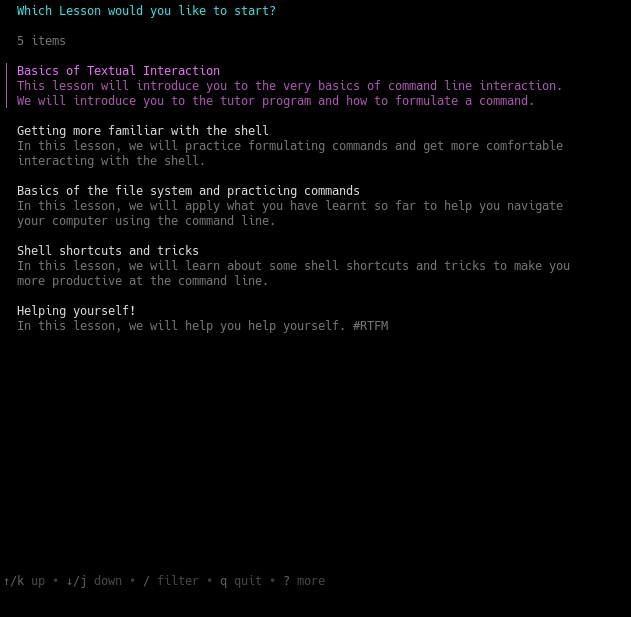
\includegraphics[width=0.9\textwidth]{img/menushort}
	\caption{Screenshot of \textit{CLI-Tutor} menu screen.}
	\label{fig:clitutormenu}
\end{figure}


\paragraph{Lesson view.} The lesson view is where the shell environment is
reproduced. It is designed to look exactly like what interacting with the shell
in a terminal looks like but with some added cues from the lesson. These cues
include the current task, its instructions and any feedback about the last
input of the user (see: \autoref{fig:lessonview}). The lesson view is also
running a \textit{Go} \textit{readline} library to provide a user input
mechanism essentially identical to that of a normal shell. The expected
shortcuts all work as they should but certain controls such as \textit{Ctrl+d},
\textit{Ctrl+z} and the \textit{Ctrl+c} interrupts are captured and ignored in
order to not close the program unexpectedly.

\begin{figure}[htbp]
	% \begin{figure}[H]
	\centering
	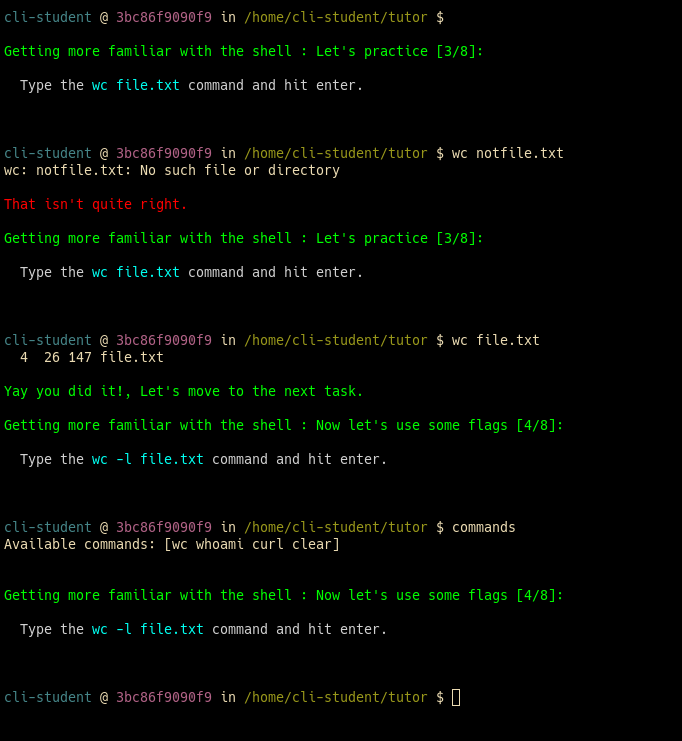
\includegraphics[width=0.9\textwidth]{img/lessonview}
	\caption{Screenshot of the \textit{CLI-Tutor} lesson view showing the task tracker, feedback mechanism and an inbuilt helper command.}
	\label{fig:lessonview}
\end{figure}


\paragraph{Mouse support.} To make the program more usable for
individuals used to GUIs, basic mouse support had to be implemented in
\textit{CLI-Tutor}. Mouse support is a bit extended in the menu than what would
be common in most TUI applications. The user can hover to highlight and click
to select a lesson. The hitboxes for the menu items are also precisely
calculated based on the text rendered to offer a consistent and GUI-like mouse
experience. In the lesson view, mouse support is implemented to a degree but
still retains the goal of providing an honest shell-like experience. The user
can access the scrollback buffer and use the mouse to select and copy text
using the keyboard shortcuts of their terminal emulator. In the web version, a
right-click menu that is native to the browser is also available.

\paragraph{Keyboard shortcuts (multiple for same).} As shown in
\autoref{fig:lessonview}, some inbuilt commands available to the user, are
not shell commands. For example, the \textit{commands} command prints all the
available commands, also known as the lesson's \textit{vocabulary}, to the
screen. There are other special commands in the lesson view that allow the user
to navigate forward and backwards through the lesson, quit the lesson and
toggle \textit{zen-mode}.

\paragraph{Zen mode.} This is a special output printing mode of the lesson
view. While not something available by default in a shell, this feature aims to
prevent the user from being overwhelmed by long textual output alongside the
lesson instructions. When \textit{zen-mode} is activated, the screen clears
itself before the output of every command. This has the effect of leaving only
the latest output and task on the screen. This feature is activated by default
in the very first lesson but then deactivated unless specifically set once the
user has been taught about clearing the screen using the \textit{clear}
command.

\paragraph{Feedback colouring.} \textit{CLI-Tutor} utilises colour to
differentiate different elements of the lesson. For example, a cyan colour is
used to indicate commands, green is used for the task tracker, yellow is used
for notes or information about key bindings and finally success and failure
feedback is also coded in red and green respectively (see:
\autoref{fig:lessonview} and \autoref{fig:colours}). In addition to colour,
text formatting elements such as the use of bold and italic text is also
utilised to form visual hierarchies and to attract the user's attention.


\subsection{Safety Considerations}

\paragraph{Fake jail warden.} To minimise the disruptions caused by
file permissions issues that may be completely cryptic to the user
\textit{CLI-Tutor}  uses a fake jail to prevent the current working directory
from being moved above the home folder of the user.

\paragraph{Sandbox.} In addition to permissions issues which are merely an
inconvenience, accidental file deletion or other potential mistakes during a
file system lesson can result in permanent data loss. To mitigate this risk and
to create a safe "sandbox" for users to use the application. The simplest
way is to run the application in a \textit{docker}\cite{dockerinc_2022}
container. However, this greatly increases the barrier of entry to using
\textit{CLI-Tutor}. To make the tool accessible and easy to distribute
a web application to serve instances of \textit{docker} containers running
\textit{CLI-Tutor} was created.

\section{Web Application}

While the core component of \textit{CLI-Tutor} is a command line application it
does have an accompanying web application (see: \autoref{fig:webversion}). The
purpose of creating this web application was briefly discussed in the preceding
section. The web application was the medium through which the user study was
conducted. Two versions of the web application were created to support the two
user groups in the user study (see: \autoref{chap:userstudy}). One version
contains the \textit{CLI-Tutor} program and the second "CLI only" version (see: \autoref{fig:cliversion})
serves to provide a sandboxed Linux shell to individuals participating in the
user study. Additionally, also to support the User Study a documentation static
website (see: \autoref{fig:docsweb}) was also created alongside the web application. In this section, we
will describe the general architecture of the application. More technical
details will be discussed in \autoref{chap:design}.


\begin{figure}[htbp]
	\centering
	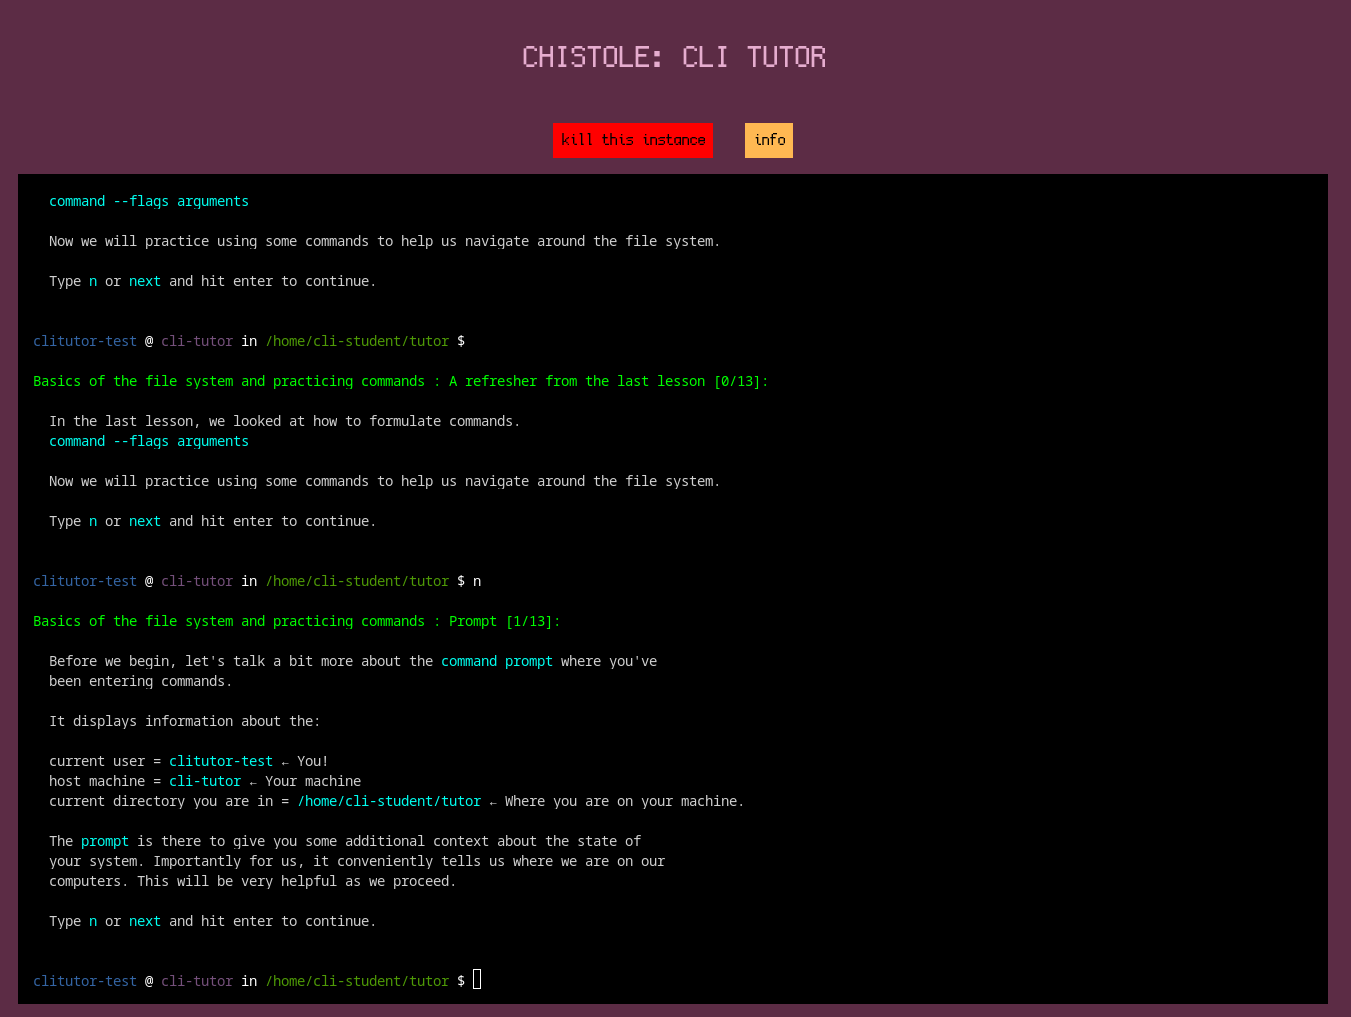
\includegraphics[width=1\textwidth]{img/cliwebshort}
	\caption{Screenshot of \textit{CLI-Tutor} running in a browser.}
	\label{fig:webversion}
\end{figure}

\begin{figure}[htbp]
	\centering
	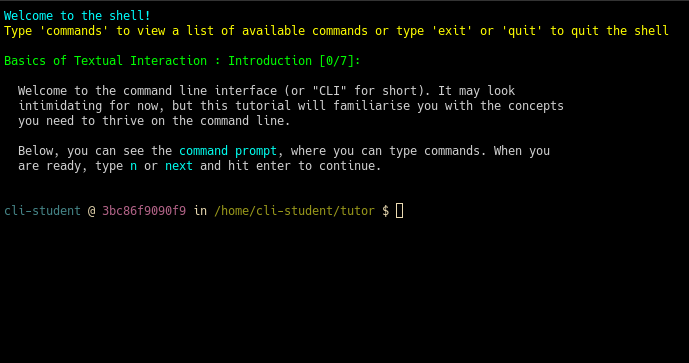
\includegraphics[width=0.9\textwidth]{img/lesson1.1}
	\caption{Screenshot of \textit{CLI-Tutor} showcasing the usage of colours.}
	\label{fig:colours}
\end{figure}

\begin{figure}[htbp]
	\centering
	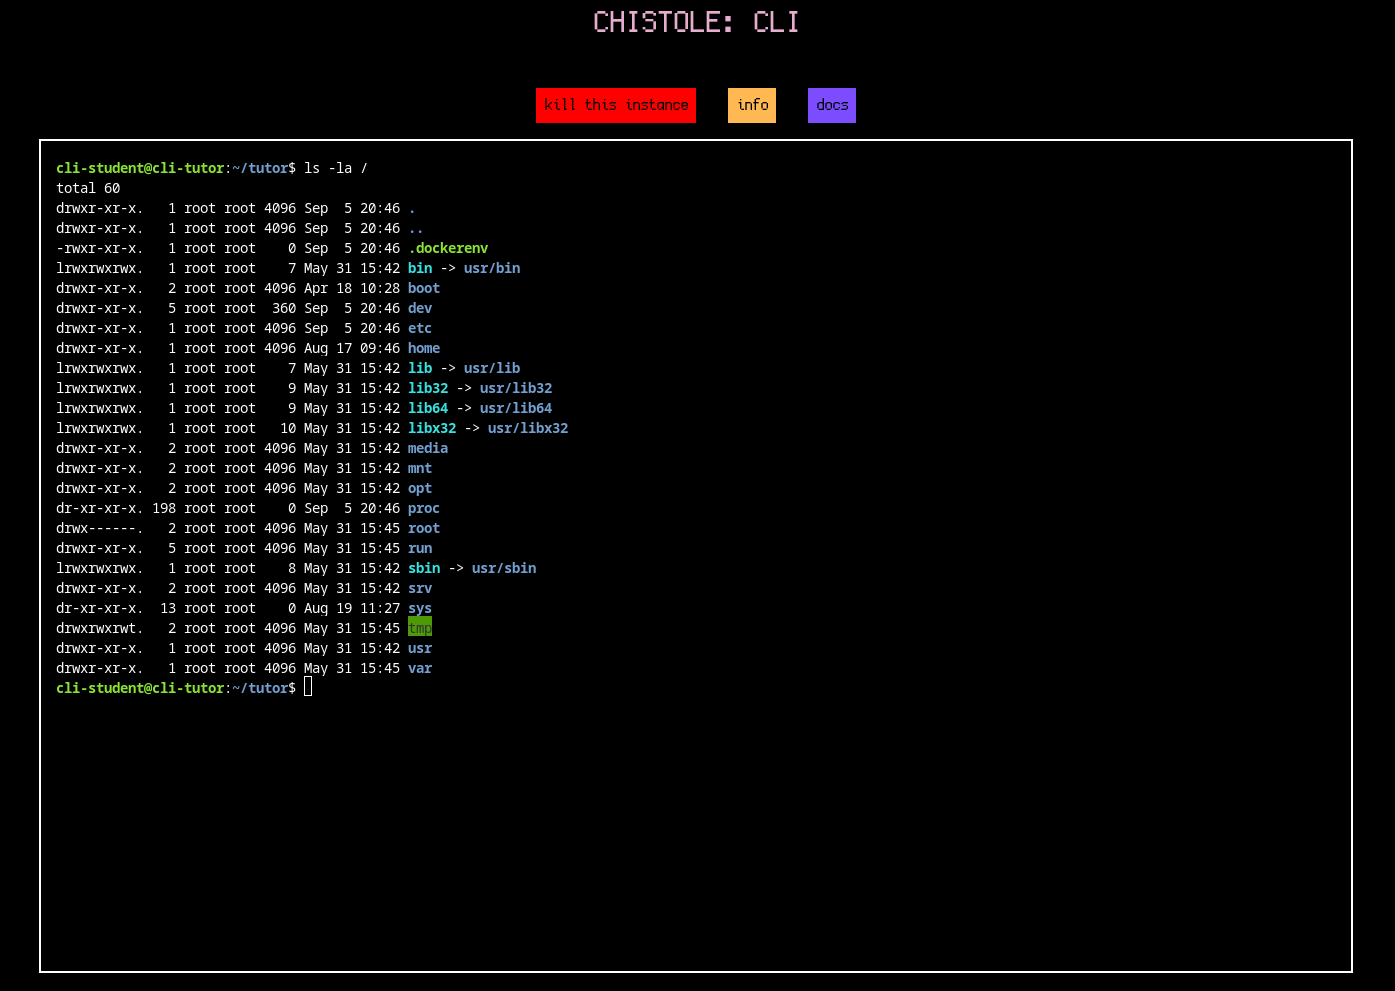
\includegraphics[width=1\textwidth]{img/clionly}
	\caption{Screenshot of the CLI only version.}
	\label{fig:welcomedocs}
\end{figure}
\begin{figure}[htbp]
	\centering
	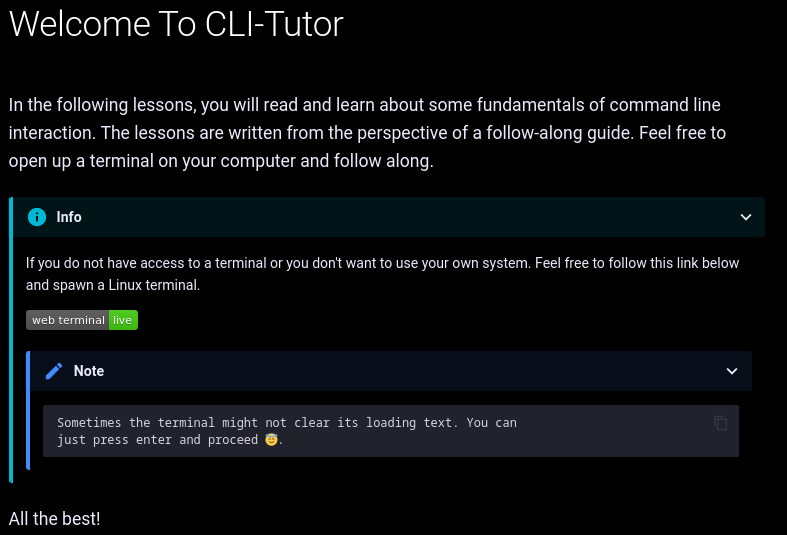
\includegraphics[width=0.85\textwidth]{img/docswelcomedark}
	\caption{Screenshot of the welcome screen of the documentation website, linking to the CLI-only version.}
	\label{fig:cliversion}
\end{figure}

\begin{figure}[htbp]
	\centering
	\includegraphics[width=0.95\textwidth]{img/docs1dark}
	\includegraphics[width=0.95\textwidth]{img/docs1light}
	\caption{Screenshots of the documentation website showcasing both light and dark modes.}
	\label{fig:docsweb}
\end{figure}

\chapter{Design And Implementation}
% - Design and Implementation
%   - overview
%   - original tinkering and considerations
%   - features and considerations
%   - architecture of cli-tool
%   - architecture of web-tool
\label{chap:design}
\section{Overview}
% Libs and tools used

\section{Architecture}
\section{Extending}
\subsubsection{Subsubsection}

\paragraph{Paragraph.} Always with a point.



\chapter{User Study}
% - User Study
%    - methodology
%       - assignment
%       - survey structure
%    - participants
% DATAPOINTS: Interest in interactive learnign or percentage of people who find
% it more effective than reading
\label{chap:userstudy}

In order to test and validate the effectiveness of our solution, a user study
was conducted. The goal of this user study was two part. Firstly, we were
interested in assessing the usability and response to \textit{CLI-Tutor}.
Secondly, we wanted to ascertain if interactive learning would be a more
effective medium to teach command line interaction than the traditional means
such as online documentation or books. In this chapter, we will describe our
user study in detail.

\section{Methodology}

The user study for this thesis work was conducted remotely and asynchronously.
We designed an online survey using the \textit{LimeSurvey}\cite{schmitzlime}
tool made available to us by the University of Zurich.

The focus of the user study was primarily on the comparison between interactive
learning approaches such as that of \textit{CLI-Tutor} and traditional ones,
which are mostly reading based. In the modern software development space,
online documentation is the status quo and the medium we choose to compare our
solution against. As discussed in \autoref{chap:design}, \textit{CLI-Tutor}
uses \textit{Markdown} to specify lessons. Many static documentation generation
websites use Markdown files to generate documentation from. This is also true
for our chosen generator. This enables us to objectively compare the
interaction medium rather than the lesson content, since the exact same lessons
can be used in both tools. Furthermore, due to the popularity of
\textit{MkDocs} it is a very realistic representation of documentation that
individuals may encounter in the wild.


\subsection{Interactive versus Non-interactive}

We designed our user study with the intention to perform an A/B style testing
comparing learning mediums. To support this we used the pseudorandom number
generation feature of \textit{LimeSurvey} to assign our participants to one of
two groups, interactive and non-interactive.

\subsection{Structure}

In this section, we provide a structural overview of our online survey. The
entire survey is available in \autoref{chap:appendixa}.

Our online survey was divided into the following sections:

\begin{itemize}

	\item User Familiarity: In this section, users answered questions relating
	      to their experience, interest and preferences to provide us with some
	      insights on each individual participant.

	\item Assignment: All participants where divided into one of two groups,
	      interactive and non-interactive. The assignment value is unknown to the
	      participant at the time of starting the survey. Our survey tool then
	      conditionally rendered a URL for the participants to follow to the next
	      section of the survey.

	\item Tutorial: At this stage, once the participants have been assigned to
	      one of the two groups, they will either be sent to our web application
	      running \textit{CLI-Tutor} or to our documentation website. If assigned
	      to the non-interactive group participants were also given the option of
	      navigating to the  \textit{CLI-only} version of our tool, in case they
	      did not have access to a Unix-like terminal (see:
	      \autoref{fig:cliversion}).

	\item Evaluation: The evaluation stage is where participants were asked a
	      series of basic questions relating to the lessons they took in the
	      previous stage. Questions were a mixture of multiple choice and free
	      text questions. This section was identical for both user groups as the
	      lessons were also identical.

	\item Feedback: In this section participants were able to provide feedback
	      regarding their experience. All but one of the questions in this
	      section were identical for both user groups. The non-interactive group
	      were asked one additional question regarding interactive learning:
	      \textit{Do you think an interactive command line tutorial application
		      would improve the learning process?}

	\item Feedback Opposite (optional): This section was optional and included
	      only one quick feedback question. At the end of the survey,
	      participants were then given a chance to try out the opposite tool to
	      which they were assigned for the bulk of the user study. No evaluation
	      or tutorial was mandated here and participants were given one free text
	      response to report on their feelings using the alternative tool.
\end{itemize}


\section{Participants}

In this section we will share insights we gathered from the first section of
the survey, where we asked experience, familiarity and more general questions.

In total, 34 participants took part in our user study. 19 of whom were assigned
to the interactive group and 15 to the non-interactive group. Recruitment was
primarily done through University channels though some participants were also
sourced through work email and word of mouth. While not limited to individuals
in software related fields, over 60\% (see: \autoref{fig:uniexp}) of the
participants were from technical backgrounds or currently computer science
students.

\subsection{Technical Experience}

Given the goals of \textit{CLI-Tutor}, It comes as no surprise that most of the
individuals who participated in our user study were of not very highly
experienced, though there were two outliers with over twenty years of
programming experience. Most of the participants were far less experienced with
a median experience of 3 years (see: \autoref{fig:programmingexp}). While not
very highly experienced in programming, most of our participants did come from
some sort of Computer Science or engineering background (see:
\autoref{fig:uniexp}).

\begin{figure}[H]
	\centering
	\scalebox{0.75}{%% Creator: Matplotlib, PGF backend
%%
%% To include the figure in your LaTeX document, write
%%   \input{<filename>.pgf}
%%
%% Make sure the required packages are loaded in your preamble
%%   \usepackage{pgf}
%%
%% Also ensure that all the required font packages are loaded; for instance,
%% the lmodern package is sometimes necessary when using math font.
%%   \usepackage{lmodern}
%%
%% Figures using additional raster images can only be included by \input if
%% they are in the same directory as the main LaTeX file. For loading figures
%% from other directories you can use the `import` package
%%   \usepackage{import}
%%
%% and then include the figures with
%%   \import{<path to file>}{<filename>.pgf}
%%
%% Matplotlib used the following preamble
%%   \usepackage{fontspec}
%%   \setmainfont{DejaVuSerif.ttf}[Path=\detokenize{/home/spam/miniconda3/envs/mpl/lib/python3.10/site-packages/matplotlib/mpl-data/fonts/ttf/}]
%%   \setsansfont{DejaVuSans.ttf}[Path=\detokenize{/home/spam/miniconda3/envs/mpl/lib/python3.10/site-packages/matplotlib/mpl-data/fonts/ttf/}]
%%   \setmonofont{DejaVuSansMono.ttf}[Path=\detokenize{/home/spam/miniconda3/envs/mpl/lib/python3.10/site-packages/matplotlib/mpl-data/fonts/ttf/}]
%%
\begingroup%
\makeatletter%
\begin{pgfpicture}%
\pgfpathrectangle{\pgfpointorigin}{\pgfqpoint{8.799314in}{3.116660in}}%
\pgfusepath{use as bounding box, clip}%
\begin{pgfscope}%
\pgfsetbuttcap%
\pgfsetmiterjoin%
\pgfsetlinewidth{0.000000pt}%
\definecolor{currentstroke}{rgb}{0.000000,0.000000,0.000000}%
\pgfsetstrokecolor{currentstroke}%
\pgfsetstrokeopacity{0.000000}%
\pgfsetdash{}{0pt}%
\pgfpathmoveto{\pgfqpoint{0.000000in}{0.000000in}}%
\pgfpathlineto{\pgfqpoint{8.799314in}{0.000000in}}%
\pgfpathlineto{\pgfqpoint{8.799314in}{3.116660in}}%
\pgfpathlineto{\pgfqpoint{0.000000in}{3.116660in}}%
\pgfpathlineto{\pgfqpoint{0.000000in}{0.000000in}}%
\pgfpathclose%
\pgfusepath{}%
\end{pgfscope}%
\begin{pgfscope}%
\pgfsetbuttcap%
\pgfsetmiterjoin%
\definecolor{currentfill}{rgb}{0.501961,0.694118,0.827451}%
\pgfsetfillcolor{currentfill}%
\pgfsetlinewidth{1.003750pt}%
\definecolor{currentstroke}{rgb}{1.000000,1.000000,1.000000}%
\pgfsetstrokecolor{currentstroke}%
\pgfsetdash{}{0pt}%
\pgfpathmoveto{\pgfqpoint{3.894914in}{1.314902in}}%
\pgfpathcurveto{\pgfqpoint{3.894914in}{1.442534in}}{\pgfqpoint{3.869773in}{1.568924in}}{\pgfqpoint{3.820931in}{1.686841in}}%
\pgfpathcurveto{\pgfqpoint{3.772088in}{1.804757in}}{\pgfqpoint{3.700494in}{1.911906in}}{\pgfqpoint{3.610245in}{2.002155in}}%
\pgfpathcurveto{\pgfqpoint{3.519995in}{2.092404in}}{\pgfqpoint{3.412847in}{2.163998in}}{\pgfqpoint{3.294931in}{2.212841in}}%
\pgfpathcurveto{\pgfqpoint{3.177014in}{2.261683in}}{\pgfqpoint{3.050624in}{2.286824in}}{\pgfqpoint{2.922992in}{2.286824in}}%
\pgfpathcurveto{\pgfqpoint{2.795361in}{2.286824in}}{\pgfqpoint{2.668970in}{2.261683in}}{\pgfqpoint{2.551054in}{2.212841in}}%
\pgfpathcurveto{\pgfqpoint{2.433138in}{2.163998in}}{\pgfqpoint{2.325989in}{2.092404in}}{\pgfqpoint{2.235740in}{2.002155in}}%
\pgfpathcurveto{\pgfqpoint{2.145491in}{1.911906in}}{\pgfqpoint{2.073896in}{1.804757in}}{\pgfqpoint{2.025054in}{1.686841in}}%
\pgfpathcurveto{\pgfqpoint{1.976211in}{1.568924in}}{\pgfqpoint{1.951070in}{1.442534in}}{\pgfqpoint{1.951070in}{1.314902in}}%
\pgfpathcurveto{\pgfqpoint{1.951070in}{1.187271in}}{\pgfqpoint{1.976211in}{1.060880in}}{\pgfqpoint{2.025054in}{0.942964in}}%
\pgfpathcurveto{\pgfqpoint{2.073896in}{0.825048in}}{\pgfqpoint{2.145491in}{0.717899in}}{\pgfqpoint{2.235740in}{0.627650in}}%
\pgfpathcurveto{\pgfqpoint{2.325989in}{0.537401in}}{\pgfqpoint{2.433138in}{0.465806in}}{\pgfqpoint{2.551054in}{0.416964in}}%
\pgfpathcurveto{\pgfqpoint{2.668970in}{0.368121in}}{\pgfqpoint{2.795361in}{0.342980in}}{\pgfqpoint{2.922992in}{0.342980in}}%
\pgfpathcurveto{\pgfqpoint{3.050624in}{0.342980in}}{\pgfqpoint{3.177014in}{0.368121in}}{\pgfqpoint{3.294931in}{0.416964in}}%
\pgfpathcurveto{\pgfqpoint{3.412847in}{0.465806in}}{\pgfqpoint{3.519995in}{0.537401in}}{\pgfqpoint{3.610245in}{0.627650in}}%
\pgfpathcurveto{\pgfqpoint{3.700494in}{0.717899in}}{\pgfqpoint{3.772088in}{0.825048in}}{\pgfqpoint{3.820931in}{0.942964in}}%
\pgfpathcurveto{\pgfqpoint{3.869773in}{1.060880in}}{\pgfqpoint{3.894914in}{1.187271in}}{\pgfqpoint{3.894914in}{1.314902in}}%
\pgfpathmoveto{\pgfqpoint{2.922992in}{1.314902in}}%
\pgfpathmoveto{\pgfqpoint{3.894914in}{1.314902in}}%
\pgfpathlineto{\pgfqpoint{3.894914in}{1.314902in}}%
\pgfpathclose%
\pgfusepath{stroke,fill}%
\end{pgfscope}%
\begin{pgfscope}%
\pgfsetbuttcap%
\pgfsetmiterjoin%
\definecolor{currentfill}{rgb}{0.992157,0.705882,0.384314}%
\pgfsetfillcolor{currentfill}%
\pgfsetlinewidth{1.003750pt}%
\definecolor{currentstroke}{rgb}{1.000000,1.000000,1.000000}%
\pgfsetstrokecolor{currentstroke}%
\pgfsetdash{}{0pt}%
\pgfpathmoveto{\pgfqpoint{2.922992in}{2.286824in}}%
\pgfpathcurveto{\pgfqpoint{2.922992in}{2.286824in}}{\pgfqpoint{2.922992in}{2.286824in}}{\pgfqpoint{2.922992in}{2.286824in}}%
\pgfpathlineto{\pgfqpoint{2.922992in}{1.314902in}}%
\pgfpathlineto{\pgfqpoint{2.922992in}{2.286824in}}%
\pgfpathlineto{\pgfqpoint{2.922992in}{2.286824in}}%
\pgfpathclose%
\pgfusepath{stroke,fill}%
\end{pgfscope}%
\begin{pgfscope}%
\definecolor{textcolor}{rgb}{0.150000,0.150000,0.150000}%
\pgfsetstrokecolor{textcolor}%
\pgfsetfillcolor{textcolor}%
\pgftext[x=2.922992in,y=0.731749in,,]{\color{textcolor}\sffamily\fontsize{12.000000}{14.400000}\selectfont 100.00\%}%
\end{pgfscope}%
\begin{pgfscope}%
\definecolor{textcolor}{rgb}{0.150000,0.150000,0.150000}%
\pgfsetstrokecolor{textcolor}%
\pgfsetfillcolor{textcolor}%
\pgftext[x=2.922992in,y=1.898055in,,]{\color{textcolor}\sffamily\fontsize{12.000000}{14.400000}\selectfont 0.00\%}%
\end{pgfscope}%
\begin{pgfscope}%
\definecolor{textcolor}{rgb}{0.000000,0.000000,0.000000}%
\pgfsetstrokecolor{textcolor}%
\pgfsetfillcolor{textcolor}%
\pgftext[x=2.922992in,y=2.613138in,,base]{\color{textcolor}\sffamily\fontsize{12.000000}{14.400000}\selectfont CLI-Tutor}%
\end{pgfscope}%
\begin{pgfscope}%
\pgfsetbuttcap%
\pgfsetmiterjoin%
\definecolor{currentfill}{rgb}{0.501961,0.694118,0.827451}%
\pgfsetfillcolor{currentfill}%
\pgfsetlinewidth{1.003750pt}%
\definecolor{currentstroke}{rgb}{1.000000,1.000000,1.000000}%
\pgfsetstrokecolor{currentstroke}%
\pgfsetdash{}{0pt}%
\pgfpathmoveto{\pgfqpoint{5.876322in}{2.286824in}}%
\pgfpathcurveto{\pgfqpoint{5.725984in}{2.286824in}}{\pgfqpoint{5.577676in}{2.251942in}}{\pgfqpoint{5.443099in}{2.184931in}}%
\pgfpathcurveto{\pgfqpoint{5.308522in}{2.117920in}}{\pgfqpoint{5.191311in}{2.020588in}}{\pgfqpoint{5.100712in}{1.900616in}}%
\pgfpathcurveto{\pgfqpoint{5.010113in}{1.780644in}}{\pgfqpoint{4.948574in}{1.641271in}}{\pgfqpoint{4.920949in}{1.493492in}}%
\pgfpathcurveto{\pgfqpoint{4.893325in}{1.345714in}}{\pgfqpoint{4.900361in}{1.193522in}}{\pgfqpoint{4.941503in}{1.048923in}}%
\pgfpathcurveto{\pgfqpoint{4.982645in}{0.904324in}}{\pgfqpoint{5.056781in}{0.771224in}}{\pgfqpoint{5.158063in}{0.660123in}}%
\pgfpathcurveto{\pgfqpoint{5.259345in}{0.549022in}}{\pgfqpoint{5.385037in}{0.462921in}}{\pgfqpoint{5.525223in}{0.408612in}}%
\pgfpathcurveto{\pgfqpoint{5.665409in}{0.354304in}}{\pgfqpoint{5.816303in}{0.333255in}}{\pgfqpoint{5.966000in}{0.347126in}}%
\pgfpathcurveto{\pgfqpoint{6.115696in}{0.360998in}}{\pgfqpoint{6.260153in}{0.409415in}}{\pgfqpoint{6.387973in}{0.488558in}}%
\pgfpathlineto{\pgfqpoint{5.876322in}{1.314902in}}%
\pgfpathlineto{\pgfqpoint{5.876322in}{2.286824in}}%
\pgfpathlineto{\pgfqpoint{5.876322in}{2.286824in}}%
\pgfpathclose%
\pgfusepath{stroke,fill}%
\end{pgfscope}%
\begin{pgfscope}%
\pgfsetbuttcap%
\pgfsetmiterjoin%
\definecolor{currentfill}{rgb}{0.992157,0.705882,0.384314}%
\pgfsetfillcolor{currentfill}%
\pgfsetlinewidth{1.003750pt}%
\definecolor{currentstroke}{rgb}{1.000000,1.000000,1.000000}%
\pgfsetstrokecolor{currentstroke}%
\pgfsetdash{}{0pt}%
\pgfpathmoveto{\pgfqpoint{6.387973in}{0.488558in}}%
\pgfpathcurveto{\pgfqpoint{6.567670in}{0.599821in}}{\pgfqpoint{6.706262in}{0.766721in}}{\pgfqpoint{6.782612in}{0.963803in}}%
\pgfpathcurveto{\pgfqpoint{6.858962in}{1.160886in}}{\pgfqpoint{6.868981in}{1.377595in}}{\pgfqpoint{6.811141in}{1.580881in}}%
\pgfpathcurveto{\pgfqpoint{6.753302in}{1.784167in}}{\pgfqpoint{6.630701in}{1.963143in}}{\pgfqpoint{6.462036in}{2.090512in}}%
\pgfpathcurveto{\pgfqpoint{6.293371in}{2.217882in}}{\pgfqpoint{6.087677in}{2.286824in}}{\pgfqpoint{5.876322in}{2.286824in}}%
\pgfpathlineto{\pgfqpoint{5.876322in}{1.314902in}}%
\pgfpathlineto{\pgfqpoint{6.387973in}{0.488558in}}%
\pgfpathlineto{\pgfqpoint{6.387973in}{0.488558in}}%
\pgfpathclose%
\pgfusepath{stroke,fill}%
\end{pgfscope}%
\begin{pgfscope}%
\definecolor{textcolor}{rgb}{0.150000,0.150000,0.150000}%
\pgfsetstrokecolor{textcolor}%
\pgfsetfillcolor{textcolor}%
\pgftext[x=5.315431in,y=1.155315in,,]{\color{textcolor}\sffamily\fontsize{12.000000}{14.400000}\selectfont 58.82\%}%
\end{pgfscope}%
\begin{pgfscope}%
\definecolor{textcolor}{rgb}{0.150000,0.150000,0.150000}%
\pgfsetstrokecolor{textcolor}%
\pgfsetfillcolor{textcolor}%
\pgftext[x=6.437214in,y=1.474490in,,]{\color{textcolor}\sffamily\fontsize{12.000000}{14.400000}\selectfont 41.18\%}%
\end{pgfscope}%
\begin{pgfscope}%
\definecolor{textcolor}{rgb}{0.000000,0.000000,0.000000}%
\pgfsetstrokecolor{textcolor}%
\pgfsetfillcolor{textcolor}%
\pgftext[x=5.876322in,y=2.613138in,,base]{\color{textcolor}\sffamily\fontsize{12.000000}{14.400000}\selectfont Non Interactive Tutor}%
\end{pgfscope}%
\begin{pgfscope}%
\definecolor{textcolor}{rgb}{0.150000,0.150000,0.150000}%
\pgfsetstrokecolor{textcolor}%
\pgfsetfillcolor{textcolor}%
\pgftext[x=4.399657in,y=3.016660in,,top]{\color{textcolor}\sffamily\fontsize{14.400000}{17.280000}\selectfont Do you feel more or less intimidated by the command line after this interactive tutor?}%
\end{pgfscope}%
\begin{pgfscope}%
\pgfsetbuttcap%
\pgfsetmiterjoin%
\definecolor{currentfill}{rgb}{1.000000,1.000000,1.000000}%
\pgfsetfillcolor{currentfill}%
\pgfsetfillopacity{0.800000}%
\pgfsetlinewidth{1.003750pt}%
\definecolor{currentstroke}{rgb}{0.800000,0.800000,0.800000}%
\pgfsetstrokecolor{currentstroke}%
\pgfsetstrokeopacity{0.800000}%
\pgfsetdash{}{0pt}%
\pgfpathmoveto{\pgfqpoint{4.031901in}{1.341726in}}%
\pgfpathlineto{\pgfqpoint{4.767413in}{1.341726in}}%
\pgfpathquadraticcurveto{\pgfqpoint{4.797969in}{1.341726in}}{\pgfqpoint{4.797969in}{1.372282in}}%
\pgfpathlineto{\pgfqpoint{4.797969in}{1.744378in}}%
\pgfpathquadraticcurveto{\pgfqpoint{4.797969in}{1.774934in}}{\pgfqpoint{4.767413in}{1.774934in}}%
\pgfpathlineto{\pgfqpoint{4.031901in}{1.774934in}}%
\pgfpathquadraticcurveto{\pgfqpoint{4.001346in}{1.774934in}}{\pgfqpoint{4.001346in}{1.744378in}}%
\pgfpathlineto{\pgfqpoint{4.001346in}{1.372282in}}%
\pgfpathquadraticcurveto{\pgfqpoint{4.001346in}{1.341726in}}{\pgfqpoint{4.031901in}{1.341726in}}%
\pgfpathlineto{\pgfqpoint{4.031901in}{1.341726in}}%
\pgfpathclose%
\pgfusepath{stroke,fill}%
\end{pgfscope}%
\begin{pgfscope}%
\pgfsetbuttcap%
\pgfsetmiterjoin%
\definecolor{currentfill}{rgb}{0.501961,0.694118,0.827451}%
\pgfsetfillcolor{currentfill}%
\pgfsetlinewidth{1.003750pt}%
\definecolor{currentstroke}{rgb}{1.000000,1.000000,1.000000}%
\pgfsetstrokecolor{currentstroke}%
\pgfsetdash{}{0pt}%
\pgfpathmoveto{\pgfqpoint{4.062457in}{1.597748in}}%
\pgfpathlineto{\pgfqpoint{4.368012in}{1.597748in}}%
\pgfpathlineto{\pgfqpoint{4.368012in}{1.704692in}}%
\pgfpathlineto{\pgfqpoint{4.062457in}{1.704692in}}%
\pgfpathlineto{\pgfqpoint{4.062457in}{1.597748in}}%
\pgfpathclose%
\pgfusepath{stroke,fill}%
\end{pgfscope}%
\begin{pgfscope}%
\definecolor{textcolor}{rgb}{0.150000,0.150000,0.150000}%
\pgfsetstrokecolor{textcolor}%
\pgfsetfillcolor{textcolor}%
\pgftext[x=4.490235in,y=1.597748in,left,base]{\color{textcolor}\sffamily\fontsize{11.000000}{13.200000}\selectfont Yes}%
\end{pgfscope}%
\begin{pgfscope}%
\pgfsetbuttcap%
\pgfsetmiterjoin%
\definecolor{currentfill}{rgb}{0.992157,0.705882,0.384314}%
\pgfsetfillcolor{currentfill}%
\pgfsetlinewidth{1.003750pt}%
\definecolor{currentstroke}{rgb}{1.000000,1.000000,1.000000}%
\pgfsetstrokecolor{currentstroke}%
\pgfsetdash{}{0pt}%
\pgfpathmoveto{\pgfqpoint{4.062457in}{1.434616in}}%
\pgfpathlineto{\pgfqpoint{4.368012in}{1.434616in}}%
\pgfpathlineto{\pgfqpoint{4.368012in}{1.541560in}}%
\pgfpathlineto{\pgfqpoint{4.062457in}{1.541560in}}%
\pgfpathlineto{\pgfqpoint{4.062457in}{1.434616in}}%
\pgfpathclose%
\pgfusepath{stroke,fill}%
\end{pgfscope}%
\begin{pgfscope}%
\definecolor{textcolor}{rgb}{0.150000,0.150000,0.150000}%
\pgfsetstrokecolor{textcolor}%
\pgfsetfillcolor{textcolor}%
\pgftext[x=4.490235in,y=1.434616in,left,base]{\color{textcolor}\sffamily\fontsize{11.000000}{13.200000}\selectfont No}%
\end{pgfscope}%
\end{pgfpicture}%
\makeatother%
\endgroup%
}
	\caption{The distribution of programming experience amongst study participants.}
	\label{fig:programmingexp}
\end{figure}

In the above figure, the programming experience of all the participants is
presented as a histogram. Programming experience is not a metric that can
reliably predict command line proficiency but can indicate the levels of
exposure to command line interfaces a participant may have had. In general,
most participants have been programming for 5 years or less and the most common
group was individuals who have been programming for 1 year. This makes sense as
a significant portion of participants were sourced through a recruiting email
distributed in the University of Zurich.

\begin{figure}[h]
	\centering
	\scalebox{0.8}{%% Creator: Matplotlib, PGF backend
%%
%% To include the figure in your LaTeX document, write
%%   \input{<filename>.pgf}
%%
%% Make sure the required packages are loaded in your preamble
%%   \usepackage{pgf}
%%
%% Also ensure that all the required font packages are loaded; for instance,
%% the lmodern package is sometimes necessary when using math font.
%%   \usepackage{lmodern}
%%
%% Figures using additional raster images can only be included by \input if
%% they are in the same directory as the main LaTeX file. For loading figures
%% from other directories you can use the `import` package
%%   \usepackage{import}
%%
%% and then include the figures with
%%   \import{<path to file>}{<filename>.pgf}
%%
%% Matplotlib used the following preamble
%%   \usepackage{fontspec}
%%   \setmainfont{DejaVuSerif.ttf}[Path=\detokenize{/home/spam/miniconda3/envs/mpl/lib/python3.10/site-packages/matplotlib/mpl-data/fonts/ttf/}]
%%   \setsansfont{DejaVuSans.ttf}[Path=\detokenize{/home/spam/miniconda3/envs/mpl/lib/python3.10/site-packages/matplotlib/mpl-data/fonts/ttf/}]
%%   \setmonofont{DejaVuSansMono.ttf}[Path=\detokenize{/home/spam/miniconda3/envs/mpl/lib/python3.10/site-packages/matplotlib/mpl-data/fonts/ttf/}]
%%
\begingroup%
\makeatletter%
\begin{pgfpicture}%
\pgfpathrectangle{\pgfpointorigin}{\pgfqpoint{8.799314in}{3.116660in}}%
\pgfusepath{use as bounding box, clip}%
\begin{pgfscope}%
\pgfsetbuttcap%
\pgfsetmiterjoin%
\pgfsetlinewidth{0.000000pt}%
\definecolor{currentstroke}{rgb}{0.000000,0.000000,0.000000}%
\pgfsetstrokecolor{currentstroke}%
\pgfsetstrokeopacity{0.000000}%
\pgfsetdash{}{0pt}%
\pgfpathmoveto{\pgfqpoint{0.000000in}{0.000000in}}%
\pgfpathlineto{\pgfqpoint{8.799314in}{0.000000in}}%
\pgfpathlineto{\pgfqpoint{8.799314in}{3.116660in}}%
\pgfpathlineto{\pgfqpoint{0.000000in}{3.116660in}}%
\pgfpathlineto{\pgfqpoint{0.000000in}{0.000000in}}%
\pgfpathclose%
\pgfusepath{}%
\end{pgfscope}%
\begin{pgfscope}%
\pgfsetbuttcap%
\pgfsetmiterjoin%
\definecolor{currentfill}{rgb}{0.501961,0.694118,0.827451}%
\pgfsetfillcolor{currentfill}%
\pgfsetlinewidth{1.003750pt}%
\definecolor{currentstroke}{rgb}{1.000000,1.000000,1.000000}%
\pgfsetstrokecolor{currentstroke}%
\pgfsetdash{}{0pt}%
\pgfpathmoveto{\pgfqpoint{3.894914in}{1.314902in}}%
\pgfpathcurveto{\pgfqpoint{3.894914in}{1.442534in}}{\pgfqpoint{3.869773in}{1.568924in}}{\pgfqpoint{3.820931in}{1.686841in}}%
\pgfpathcurveto{\pgfqpoint{3.772088in}{1.804757in}}{\pgfqpoint{3.700494in}{1.911906in}}{\pgfqpoint{3.610245in}{2.002155in}}%
\pgfpathcurveto{\pgfqpoint{3.519995in}{2.092404in}}{\pgfqpoint{3.412847in}{2.163998in}}{\pgfqpoint{3.294931in}{2.212841in}}%
\pgfpathcurveto{\pgfqpoint{3.177014in}{2.261683in}}{\pgfqpoint{3.050624in}{2.286824in}}{\pgfqpoint{2.922992in}{2.286824in}}%
\pgfpathcurveto{\pgfqpoint{2.795361in}{2.286824in}}{\pgfqpoint{2.668970in}{2.261683in}}{\pgfqpoint{2.551054in}{2.212841in}}%
\pgfpathcurveto{\pgfqpoint{2.433138in}{2.163998in}}{\pgfqpoint{2.325989in}{2.092404in}}{\pgfqpoint{2.235740in}{2.002155in}}%
\pgfpathcurveto{\pgfqpoint{2.145491in}{1.911906in}}{\pgfqpoint{2.073896in}{1.804757in}}{\pgfqpoint{2.025054in}{1.686841in}}%
\pgfpathcurveto{\pgfqpoint{1.976211in}{1.568924in}}{\pgfqpoint{1.951070in}{1.442534in}}{\pgfqpoint{1.951070in}{1.314902in}}%
\pgfpathcurveto{\pgfqpoint{1.951070in}{1.187271in}}{\pgfqpoint{1.976211in}{1.060880in}}{\pgfqpoint{2.025054in}{0.942964in}}%
\pgfpathcurveto{\pgfqpoint{2.073896in}{0.825048in}}{\pgfqpoint{2.145491in}{0.717899in}}{\pgfqpoint{2.235740in}{0.627650in}}%
\pgfpathcurveto{\pgfqpoint{2.325989in}{0.537401in}}{\pgfqpoint{2.433138in}{0.465806in}}{\pgfqpoint{2.551054in}{0.416964in}}%
\pgfpathcurveto{\pgfqpoint{2.668970in}{0.368121in}}{\pgfqpoint{2.795361in}{0.342980in}}{\pgfqpoint{2.922992in}{0.342980in}}%
\pgfpathcurveto{\pgfqpoint{3.050624in}{0.342980in}}{\pgfqpoint{3.177014in}{0.368121in}}{\pgfqpoint{3.294931in}{0.416964in}}%
\pgfpathcurveto{\pgfqpoint{3.412847in}{0.465806in}}{\pgfqpoint{3.519995in}{0.537401in}}{\pgfqpoint{3.610245in}{0.627650in}}%
\pgfpathcurveto{\pgfqpoint{3.700494in}{0.717899in}}{\pgfqpoint{3.772088in}{0.825048in}}{\pgfqpoint{3.820931in}{0.942964in}}%
\pgfpathcurveto{\pgfqpoint{3.869773in}{1.060880in}}{\pgfqpoint{3.894914in}{1.187271in}}{\pgfqpoint{3.894914in}{1.314902in}}%
\pgfpathmoveto{\pgfqpoint{2.922992in}{1.314902in}}%
\pgfpathmoveto{\pgfqpoint{3.894914in}{1.314902in}}%
\pgfpathlineto{\pgfqpoint{3.894914in}{1.314902in}}%
\pgfpathclose%
\pgfusepath{stroke,fill}%
\end{pgfscope}%
\begin{pgfscope}%
\pgfsetbuttcap%
\pgfsetmiterjoin%
\definecolor{currentfill}{rgb}{0.992157,0.705882,0.384314}%
\pgfsetfillcolor{currentfill}%
\pgfsetlinewidth{1.003750pt}%
\definecolor{currentstroke}{rgb}{1.000000,1.000000,1.000000}%
\pgfsetstrokecolor{currentstroke}%
\pgfsetdash{}{0pt}%
\pgfpathmoveto{\pgfqpoint{2.922992in}{2.286824in}}%
\pgfpathcurveto{\pgfqpoint{2.922992in}{2.286824in}}{\pgfqpoint{2.922992in}{2.286824in}}{\pgfqpoint{2.922992in}{2.286824in}}%
\pgfpathlineto{\pgfqpoint{2.922992in}{1.314902in}}%
\pgfpathlineto{\pgfqpoint{2.922992in}{2.286824in}}%
\pgfpathlineto{\pgfqpoint{2.922992in}{2.286824in}}%
\pgfpathclose%
\pgfusepath{stroke,fill}%
\end{pgfscope}%
\begin{pgfscope}%
\definecolor{textcolor}{rgb}{0.150000,0.150000,0.150000}%
\pgfsetstrokecolor{textcolor}%
\pgfsetfillcolor{textcolor}%
\pgftext[x=2.922992in,y=0.731749in,,]{\color{textcolor}\sffamily\fontsize{12.000000}{14.400000}\selectfont 100.00\%}%
\end{pgfscope}%
\begin{pgfscope}%
\definecolor{textcolor}{rgb}{0.150000,0.150000,0.150000}%
\pgfsetstrokecolor{textcolor}%
\pgfsetfillcolor{textcolor}%
\pgftext[x=2.922992in,y=1.898055in,,]{\color{textcolor}\sffamily\fontsize{12.000000}{14.400000}\selectfont 0.00\%}%
\end{pgfscope}%
\begin{pgfscope}%
\definecolor{textcolor}{rgb}{0.000000,0.000000,0.000000}%
\pgfsetstrokecolor{textcolor}%
\pgfsetfillcolor{textcolor}%
\pgftext[x=2.922992in,y=2.613138in,,base]{\color{textcolor}\sffamily\fontsize{12.000000}{14.400000}\selectfont CLI-Tutor}%
\end{pgfscope}%
\begin{pgfscope}%
\pgfsetbuttcap%
\pgfsetmiterjoin%
\definecolor{currentfill}{rgb}{0.501961,0.694118,0.827451}%
\pgfsetfillcolor{currentfill}%
\pgfsetlinewidth{1.003750pt}%
\definecolor{currentstroke}{rgb}{1.000000,1.000000,1.000000}%
\pgfsetstrokecolor{currentstroke}%
\pgfsetdash{}{0pt}%
\pgfpathmoveto{\pgfqpoint{5.876322in}{2.286824in}}%
\pgfpathcurveto{\pgfqpoint{5.725984in}{2.286824in}}{\pgfqpoint{5.577676in}{2.251942in}}{\pgfqpoint{5.443099in}{2.184931in}}%
\pgfpathcurveto{\pgfqpoint{5.308522in}{2.117920in}}{\pgfqpoint{5.191311in}{2.020588in}}{\pgfqpoint{5.100712in}{1.900616in}}%
\pgfpathcurveto{\pgfqpoint{5.010113in}{1.780644in}}{\pgfqpoint{4.948574in}{1.641271in}}{\pgfqpoint{4.920949in}{1.493492in}}%
\pgfpathcurveto{\pgfqpoint{4.893325in}{1.345714in}}{\pgfqpoint{4.900361in}{1.193522in}}{\pgfqpoint{4.941503in}{1.048923in}}%
\pgfpathcurveto{\pgfqpoint{4.982645in}{0.904324in}}{\pgfqpoint{5.056781in}{0.771224in}}{\pgfqpoint{5.158063in}{0.660123in}}%
\pgfpathcurveto{\pgfqpoint{5.259345in}{0.549022in}}{\pgfqpoint{5.385037in}{0.462921in}}{\pgfqpoint{5.525223in}{0.408612in}}%
\pgfpathcurveto{\pgfqpoint{5.665409in}{0.354304in}}{\pgfqpoint{5.816303in}{0.333255in}}{\pgfqpoint{5.966000in}{0.347126in}}%
\pgfpathcurveto{\pgfqpoint{6.115696in}{0.360998in}}{\pgfqpoint{6.260153in}{0.409415in}}{\pgfqpoint{6.387973in}{0.488558in}}%
\pgfpathlineto{\pgfqpoint{5.876322in}{1.314902in}}%
\pgfpathlineto{\pgfqpoint{5.876322in}{2.286824in}}%
\pgfpathlineto{\pgfqpoint{5.876322in}{2.286824in}}%
\pgfpathclose%
\pgfusepath{stroke,fill}%
\end{pgfscope}%
\begin{pgfscope}%
\pgfsetbuttcap%
\pgfsetmiterjoin%
\definecolor{currentfill}{rgb}{0.992157,0.705882,0.384314}%
\pgfsetfillcolor{currentfill}%
\pgfsetlinewidth{1.003750pt}%
\definecolor{currentstroke}{rgb}{1.000000,1.000000,1.000000}%
\pgfsetstrokecolor{currentstroke}%
\pgfsetdash{}{0pt}%
\pgfpathmoveto{\pgfqpoint{6.387973in}{0.488558in}}%
\pgfpathcurveto{\pgfqpoint{6.567670in}{0.599821in}}{\pgfqpoint{6.706262in}{0.766721in}}{\pgfqpoint{6.782612in}{0.963803in}}%
\pgfpathcurveto{\pgfqpoint{6.858962in}{1.160886in}}{\pgfqpoint{6.868981in}{1.377595in}}{\pgfqpoint{6.811141in}{1.580881in}}%
\pgfpathcurveto{\pgfqpoint{6.753302in}{1.784167in}}{\pgfqpoint{6.630701in}{1.963143in}}{\pgfqpoint{6.462036in}{2.090512in}}%
\pgfpathcurveto{\pgfqpoint{6.293371in}{2.217882in}}{\pgfqpoint{6.087677in}{2.286824in}}{\pgfqpoint{5.876322in}{2.286824in}}%
\pgfpathlineto{\pgfqpoint{5.876322in}{1.314902in}}%
\pgfpathlineto{\pgfqpoint{6.387973in}{0.488558in}}%
\pgfpathlineto{\pgfqpoint{6.387973in}{0.488558in}}%
\pgfpathclose%
\pgfusepath{stroke,fill}%
\end{pgfscope}%
\begin{pgfscope}%
\definecolor{textcolor}{rgb}{0.150000,0.150000,0.150000}%
\pgfsetstrokecolor{textcolor}%
\pgfsetfillcolor{textcolor}%
\pgftext[x=5.315431in,y=1.155315in,,]{\color{textcolor}\sffamily\fontsize{12.000000}{14.400000}\selectfont 58.82\%}%
\end{pgfscope}%
\begin{pgfscope}%
\definecolor{textcolor}{rgb}{0.150000,0.150000,0.150000}%
\pgfsetstrokecolor{textcolor}%
\pgfsetfillcolor{textcolor}%
\pgftext[x=6.437214in,y=1.474490in,,]{\color{textcolor}\sffamily\fontsize{12.000000}{14.400000}\selectfont 41.18\%}%
\end{pgfscope}%
\begin{pgfscope}%
\definecolor{textcolor}{rgb}{0.000000,0.000000,0.000000}%
\pgfsetstrokecolor{textcolor}%
\pgfsetfillcolor{textcolor}%
\pgftext[x=5.876322in,y=2.613138in,,base]{\color{textcolor}\sffamily\fontsize{12.000000}{14.400000}\selectfont Non Interactive Tutor}%
\end{pgfscope}%
\begin{pgfscope}%
\definecolor{textcolor}{rgb}{0.150000,0.150000,0.150000}%
\pgfsetstrokecolor{textcolor}%
\pgfsetfillcolor{textcolor}%
\pgftext[x=4.399657in,y=3.016660in,,top]{\color{textcolor}\sffamily\fontsize{14.400000}{17.280000}\selectfont Do you feel more or less intimidated by the command line after this interactive tutor?}%
\end{pgfscope}%
\begin{pgfscope}%
\pgfsetbuttcap%
\pgfsetmiterjoin%
\definecolor{currentfill}{rgb}{1.000000,1.000000,1.000000}%
\pgfsetfillcolor{currentfill}%
\pgfsetfillopacity{0.800000}%
\pgfsetlinewidth{1.003750pt}%
\definecolor{currentstroke}{rgb}{0.800000,0.800000,0.800000}%
\pgfsetstrokecolor{currentstroke}%
\pgfsetstrokeopacity{0.800000}%
\pgfsetdash{}{0pt}%
\pgfpathmoveto{\pgfqpoint{4.031901in}{1.341726in}}%
\pgfpathlineto{\pgfqpoint{4.767413in}{1.341726in}}%
\pgfpathquadraticcurveto{\pgfqpoint{4.797969in}{1.341726in}}{\pgfqpoint{4.797969in}{1.372282in}}%
\pgfpathlineto{\pgfqpoint{4.797969in}{1.744378in}}%
\pgfpathquadraticcurveto{\pgfqpoint{4.797969in}{1.774934in}}{\pgfqpoint{4.767413in}{1.774934in}}%
\pgfpathlineto{\pgfqpoint{4.031901in}{1.774934in}}%
\pgfpathquadraticcurveto{\pgfqpoint{4.001346in}{1.774934in}}{\pgfqpoint{4.001346in}{1.744378in}}%
\pgfpathlineto{\pgfqpoint{4.001346in}{1.372282in}}%
\pgfpathquadraticcurveto{\pgfqpoint{4.001346in}{1.341726in}}{\pgfqpoint{4.031901in}{1.341726in}}%
\pgfpathlineto{\pgfqpoint{4.031901in}{1.341726in}}%
\pgfpathclose%
\pgfusepath{stroke,fill}%
\end{pgfscope}%
\begin{pgfscope}%
\pgfsetbuttcap%
\pgfsetmiterjoin%
\definecolor{currentfill}{rgb}{0.501961,0.694118,0.827451}%
\pgfsetfillcolor{currentfill}%
\pgfsetlinewidth{1.003750pt}%
\definecolor{currentstroke}{rgb}{1.000000,1.000000,1.000000}%
\pgfsetstrokecolor{currentstroke}%
\pgfsetdash{}{0pt}%
\pgfpathmoveto{\pgfqpoint{4.062457in}{1.597748in}}%
\pgfpathlineto{\pgfqpoint{4.368012in}{1.597748in}}%
\pgfpathlineto{\pgfqpoint{4.368012in}{1.704692in}}%
\pgfpathlineto{\pgfqpoint{4.062457in}{1.704692in}}%
\pgfpathlineto{\pgfqpoint{4.062457in}{1.597748in}}%
\pgfpathclose%
\pgfusepath{stroke,fill}%
\end{pgfscope}%
\begin{pgfscope}%
\definecolor{textcolor}{rgb}{0.150000,0.150000,0.150000}%
\pgfsetstrokecolor{textcolor}%
\pgfsetfillcolor{textcolor}%
\pgftext[x=4.490235in,y=1.597748in,left,base]{\color{textcolor}\sffamily\fontsize{11.000000}{13.200000}\selectfont Yes}%
\end{pgfscope}%
\begin{pgfscope}%
\pgfsetbuttcap%
\pgfsetmiterjoin%
\definecolor{currentfill}{rgb}{0.992157,0.705882,0.384314}%
\pgfsetfillcolor{currentfill}%
\pgfsetlinewidth{1.003750pt}%
\definecolor{currentstroke}{rgb}{1.000000,1.000000,1.000000}%
\pgfsetstrokecolor{currentstroke}%
\pgfsetdash{}{0pt}%
\pgfpathmoveto{\pgfqpoint{4.062457in}{1.434616in}}%
\pgfpathlineto{\pgfqpoint{4.368012in}{1.434616in}}%
\pgfpathlineto{\pgfqpoint{4.368012in}{1.541560in}}%
\pgfpathlineto{\pgfqpoint{4.062457in}{1.541560in}}%
\pgfpathlineto{\pgfqpoint{4.062457in}{1.434616in}}%
\pgfpathclose%
\pgfusepath{stroke,fill}%
\end{pgfscope}%
\begin{pgfscope}%
\definecolor{textcolor}{rgb}{0.150000,0.150000,0.150000}%
\pgfsetstrokecolor{textcolor}%
\pgfsetfillcolor{textcolor}%
\pgftext[x=4.490235in,y=1.434616in,left,base]{\color{textcolor}\sffamily\fontsize{11.000000}{13.200000}\selectfont No}%
\end{pgfscope}%
\end{pgfpicture}%
\makeatother%
\endgroup%
}
	\caption{University level Computer Science experience amongst study participants.}
	\label{fig:uniexp}
\end{figure}

%TODO: SEE IF FOLLOWING PAGE THING HOLDS
Participants were also asked about whether they had any University experience
in Computer Science or related fields. Most participants had some degree of
experience at the Bachelor's and Master's level but despite this 29.32\%
reported not having any university experience in Computer Science. The complete
distribution across all levels of university experience can be found on the following page in
\autoref{fig:uniexp}.

\FloatBarrier %TODO: SEE IF THIS IS NECESSARY


\subsection{Feelings about the CLIs}

To gauge interest and feelings, questions regarding interest and comfort level
with CLIs were also asked. In general the interest in integrating the command
line more into day to day computer use was high. With 79.41\% (see:
\autoref{fig:daytoday}) of respondents reporting that they were interested in
doing so. Participants were also asked to explain their motivations.
Motivations were varied, but there were some commonalities in the motivations
to integrate CLIs more in daily computer usage. For some, the motivation was a
curiosity about getting to know their computers better:

\begin{quotes}
	"It is an additional tool, where one can learn and do a myriad of things with while also
	improving one's understanding of computer systems as a whole."
\end{quotes}

\begin{quotes}
	"to build up a better understanding of how things work behind the scenes."
\end{quotes}

For one respondent, this sentiment was even partially altruistic.

\begin{quotes}
	"For using to fix ppl's and my computer if it breaks/bugs out"
\end{quotes}

Other sentiments expressed interest in integrating CLIs more in the work
environment as a productivity booster or as an important skill.


\begin{quotes}
	"Due to my field of work, more familiarity and proficiency with any CLI would be helpful"
\end{quotes}

\begin{quotes}
	"to optimize the workflow"
\end{quotes}

\begin{quotes}
	"It't much easier to replicate/reproduce the results than using GUI"
\end{quotes}

\begin{figure}[htbp]
	\scalebox{0.65}{%% Creator: Matplotlib, PGF backend
%%
%% To include the figure in your LaTeX document, write
%%   \input{<filename>.pgf}
%%
%% Make sure the required packages are loaded in your preamble
%%   \usepackage{pgf}
%%
%% Also ensure that all the required font packages are loaded; for instance,
%% the lmodern package is sometimes necessary when using math font.
%%   \usepackage{lmodern}
%%
%% Figures using additional raster images can only be included by \input if
%% they are in the same directory as the main LaTeX file. For loading figures
%% from other directories you can use the `import` package
%%   \usepackage{import}
%%
%% and then include the figures with
%%   \import{<path to file>}{<filename>.pgf}
%%
%% Matplotlib used the following preamble
%%   \usepackage{fontspec}
%%   \setmainfont{DejaVuSerif.ttf}[Path=\detokenize{/home/spam/miniconda3/envs/mpl/lib/python3.10/site-packages/matplotlib/mpl-data/fonts/ttf/}]
%%   \setsansfont{DejaVuSans.ttf}[Path=\detokenize{/home/spam/miniconda3/envs/mpl/lib/python3.10/site-packages/matplotlib/mpl-data/fonts/ttf/}]
%%   \setmonofont{DejaVuSansMono.ttf}[Path=\detokenize{/home/spam/miniconda3/envs/mpl/lib/python3.10/site-packages/matplotlib/mpl-data/fonts/ttf/}]
%%
\begingroup%
\makeatletter%
\begin{pgfpicture}%
\pgfpathrectangle{\pgfpointorigin}{\pgfqpoint{8.799314in}{3.116660in}}%
\pgfusepath{use as bounding box, clip}%
\begin{pgfscope}%
\pgfsetbuttcap%
\pgfsetmiterjoin%
\pgfsetlinewidth{0.000000pt}%
\definecolor{currentstroke}{rgb}{0.000000,0.000000,0.000000}%
\pgfsetstrokecolor{currentstroke}%
\pgfsetstrokeopacity{0.000000}%
\pgfsetdash{}{0pt}%
\pgfpathmoveto{\pgfqpoint{0.000000in}{0.000000in}}%
\pgfpathlineto{\pgfqpoint{8.799314in}{0.000000in}}%
\pgfpathlineto{\pgfqpoint{8.799314in}{3.116660in}}%
\pgfpathlineto{\pgfqpoint{0.000000in}{3.116660in}}%
\pgfpathlineto{\pgfqpoint{0.000000in}{0.000000in}}%
\pgfpathclose%
\pgfusepath{}%
\end{pgfscope}%
\begin{pgfscope}%
\pgfsetbuttcap%
\pgfsetmiterjoin%
\definecolor{currentfill}{rgb}{0.501961,0.694118,0.827451}%
\pgfsetfillcolor{currentfill}%
\pgfsetlinewidth{1.003750pt}%
\definecolor{currentstroke}{rgb}{1.000000,1.000000,1.000000}%
\pgfsetstrokecolor{currentstroke}%
\pgfsetdash{}{0pt}%
\pgfpathmoveto{\pgfqpoint{3.894914in}{1.314902in}}%
\pgfpathcurveto{\pgfqpoint{3.894914in}{1.442534in}}{\pgfqpoint{3.869773in}{1.568924in}}{\pgfqpoint{3.820931in}{1.686841in}}%
\pgfpathcurveto{\pgfqpoint{3.772088in}{1.804757in}}{\pgfqpoint{3.700494in}{1.911906in}}{\pgfqpoint{3.610245in}{2.002155in}}%
\pgfpathcurveto{\pgfqpoint{3.519995in}{2.092404in}}{\pgfqpoint{3.412847in}{2.163998in}}{\pgfqpoint{3.294931in}{2.212841in}}%
\pgfpathcurveto{\pgfqpoint{3.177014in}{2.261683in}}{\pgfqpoint{3.050624in}{2.286824in}}{\pgfqpoint{2.922992in}{2.286824in}}%
\pgfpathcurveto{\pgfqpoint{2.795361in}{2.286824in}}{\pgfqpoint{2.668970in}{2.261683in}}{\pgfqpoint{2.551054in}{2.212841in}}%
\pgfpathcurveto{\pgfqpoint{2.433138in}{2.163998in}}{\pgfqpoint{2.325989in}{2.092404in}}{\pgfqpoint{2.235740in}{2.002155in}}%
\pgfpathcurveto{\pgfqpoint{2.145491in}{1.911906in}}{\pgfqpoint{2.073896in}{1.804757in}}{\pgfqpoint{2.025054in}{1.686841in}}%
\pgfpathcurveto{\pgfqpoint{1.976211in}{1.568924in}}{\pgfqpoint{1.951070in}{1.442534in}}{\pgfqpoint{1.951070in}{1.314902in}}%
\pgfpathcurveto{\pgfqpoint{1.951070in}{1.187271in}}{\pgfqpoint{1.976211in}{1.060880in}}{\pgfqpoint{2.025054in}{0.942964in}}%
\pgfpathcurveto{\pgfqpoint{2.073896in}{0.825048in}}{\pgfqpoint{2.145491in}{0.717899in}}{\pgfqpoint{2.235740in}{0.627650in}}%
\pgfpathcurveto{\pgfqpoint{2.325989in}{0.537401in}}{\pgfqpoint{2.433138in}{0.465806in}}{\pgfqpoint{2.551054in}{0.416964in}}%
\pgfpathcurveto{\pgfqpoint{2.668970in}{0.368121in}}{\pgfqpoint{2.795361in}{0.342980in}}{\pgfqpoint{2.922992in}{0.342980in}}%
\pgfpathcurveto{\pgfqpoint{3.050624in}{0.342980in}}{\pgfqpoint{3.177014in}{0.368121in}}{\pgfqpoint{3.294931in}{0.416964in}}%
\pgfpathcurveto{\pgfqpoint{3.412847in}{0.465806in}}{\pgfqpoint{3.519995in}{0.537401in}}{\pgfqpoint{3.610245in}{0.627650in}}%
\pgfpathcurveto{\pgfqpoint{3.700494in}{0.717899in}}{\pgfqpoint{3.772088in}{0.825048in}}{\pgfqpoint{3.820931in}{0.942964in}}%
\pgfpathcurveto{\pgfqpoint{3.869773in}{1.060880in}}{\pgfqpoint{3.894914in}{1.187271in}}{\pgfqpoint{3.894914in}{1.314902in}}%
\pgfpathmoveto{\pgfqpoint{2.922992in}{1.314902in}}%
\pgfpathmoveto{\pgfqpoint{3.894914in}{1.314902in}}%
\pgfpathlineto{\pgfqpoint{3.894914in}{1.314902in}}%
\pgfpathclose%
\pgfusepath{stroke,fill}%
\end{pgfscope}%
\begin{pgfscope}%
\pgfsetbuttcap%
\pgfsetmiterjoin%
\definecolor{currentfill}{rgb}{0.992157,0.705882,0.384314}%
\pgfsetfillcolor{currentfill}%
\pgfsetlinewidth{1.003750pt}%
\definecolor{currentstroke}{rgb}{1.000000,1.000000,1.000000}%
\pgfsetstrokecolor{currentstroke}%
\pgfsetdash{}{0pt}%
\pgfpathmoveto{\pgfqpoint{2.922992in}{2.286824in}}%
\pgfpathcurveto{\pgfqpoint{2.922992in}{2.286824in}}{\pgfqpoint{2.922992in}{2.286824in}}{\pgfqpoint{2.922992in}{2.286824in}}%
\pgfpathlineto{\pgfqpoint{2.922992in}{1.314902in}}%
\pgfpathlineto{\pgfqpoint{2.922992in}{2.286824in}}%
\pgfpathlineto{\pgfqpoint{2.922992in}{2.286824in}}%
\pgfpathclose%
\pgfusepath{stroke,fill}%
\end{pgfscope}%
\begin{pgfscope}%
\definecolor{textcolor}{rgb}{0.150000,0.150000,0.150000}%
\pgfsetstrokecolor{textcolor}%
\pgfsetfillcolor{textcolor}%
\pgftext[x=2.922992in,y=0.731749in,,]{\color{textcolor}\sffamily\fontsize{12.000000}{14.400000}\selectfont 100.00\%}%
\end{pgfscope}%
\begin{pgfscope}%
\definecolor{textcolor}{rgb}{0.150000,0.150000,0.150000}%
\pgfsetstrokecolor{textcolor}%
\pgfsetfillcolor{textcolor}%
\pgftext[x=2.922992in,y=1.898055in,,]{\color{textcolor}\sffamily\fontsize{12.000000}{14.400000}\selectfont 0.00\%}%
\end{pgfscope}%
\begin{pgfscope}%
\definecolor{textcolor}{rgb}{0.000000,0.000000,0.000000}%
\pgfsetstrokecolor{textcolor}%
\pgfsetfillcolor{textcolor}%
\pgftext[x=2.922992in,y=2.613138in,,base]{\color{textcolor}\sffamily\fontsize{12.000000}{14.400000}\selectfont CLI-Tutor}%
\end{pgfscope}%
\begin{pgfscope}%
\pgfsetbuttcap%
\pgfsetmiterjoin%
\definecolor{currentfill}{rgb}{0.501961,0.694118,0.827451}%
\pgfsetfillcolor{currentfill}%
\pgfsetlinewidth{1.003750pt}%
\definecolor{currentstroke}{rgb}{1.000000,1.000000,1.000000}%
\pgfsetstrokecolor{currentstroke}%
\pgfsetdash{}{0pt}%
\pgfpathmoveto{\pgfqpoint{5.876322in}{2.286824in}}%
\pgfpathcurveto{\pgfqpoint{5.725984in}{2.286824in}}{\pgfqpoint{5.577676in}{2.251942in}}{\pgfqpoint{5.443099in}{2.184931in}}%
\pgfpathcurveto{\pgfqpoint{5.308522in}{2.117920in}}{\pgfqpoint{5.191311in}{2.020588in}}{\pgfqpoint{5.100712in}{1.900616in}}%
\pgfpathcurveto{\pgfqpoint{5.010113in}{1.780644in}}{\pgfqpoint{4.948574in}{1.641271in}}{\pgfqpoint{4.920949in}{1.493492in}}%
\pgfpathcurveto{\pgfqpoint{4.893325in}{1.345714in}}{\pgfqpoint{4.900361in}{1.193522in}}{\pgfqpoint{4.941503in}{1.048923in}}%
\pgfpathcurveto{\pgfqpoint{4.982645in}{0.904324in}}{\pgfqpoint{5.056781in}{0.771224in}}{\pgfqpoint{5.158063in}{0.660123in}}%
\pgfpathcurveto{\pgfqpoint{5.259345in}{0.549022in}}{\pgfqpoint{5.385037in}{0.462921in}}{\pgfqpoint{5.525223in}{0.408612in}}%
\pgfpathcurveto{\pgfqpoint{5.665409in}{0.354304in}}{\pgfqpoint{5.816303in}{0.333255in}}{\pgfqpoint{5.966000in}{0.347126in}}%
\pgfpathcurveto{\pgfqpoint{6.115696in}{0.360998in}}{\pgfqpoint{6.260153in}{0.409415in}}{\pgfqpoint{6.387973in}{0.488558in}}%
\pgfpathlineto{\pgfqpoint{5.876322in}{1.314902in}}%
\pgfpathlineto{\pgfqpoint{5.876322in}{2.286824in}}%
\pgfpathlineto{\pgfqpoint{5.876322in}{2.286824in}}%
\pgfpathclose%
\pgfusepath{stroke,fill}%
\end{pgfscope}%
\begin{pgfscope}%
\pgfsetbuttcap%
\pgfsetmiterjoin%
\definecolor{currentfill}{rgb}{0.992157,0.705882,0.384314}%
\pgfsetfillcolor{currentfill}%
\pgfsetlinewidth{1.003750pt}%
\definecolor{currentstroke}{rgb}{1.000000,1.000000,1.000000}%
\pgfsetstrokecolor{currentstroke}%
\pgfsetdash{}{0pt}%
\pgfpathmoveto{\pgfqpoint{6.387973in}{0.488558in}}%
\pgfpathcurveto{\pgfqpoint{6.567670in}{0.599821in}}{\pgfqpoint{6.706262in}{0.766721in}}{\pgfqpoint{6.782612in}{0.963803in}}%
\pgfpathcurveto{\pgfqpoint{6.858962in}{1.160886in}}{\pgfqpoint{6.868981in}{1.377595in}}{\pgfqpoint{6.811141in}{1.580881in}}%
\pgfpathcurveto{\pgfqpoint{6.753302in}{1.784167in}}{\pgfqpoint{6.630701in}{1.963143in}}{\pgfqpoint{6.462036in}{2.090512in}}%
\pgfpathcurveto{\pgfqpoint{6.293371in}{2.217882in}}{\pgfqpoint{6.087677in}{2.286824in}}{\pgfqpoint{5.876322in}{2.286824in}}%
\pgfpathlineto{\pgfqpoint{5.876322in}{1.314902in}}%
\pgfpathlineto{\pgfqpoint{6.387973in}{0.488558in}}%
\pgfpathlineto{\pgfqpoint{6.387973in}{0.488558in}}%
\pgfpathclose%
\pgfusepath{stroke,fill}%
\end{pgfscope}%
\begin{pgfscope}%
\definecolor{textcolor}{rgb}{0.150000,0.150000,0.150000}%
\pgfsetstrokecolor{textcolor}%
\pgfsetfillcolor{textcolor}%
\pgftext[x=5.315431in,y=1.155315in,,]{\color{textcolor}\sffamily\fontsize{12.000000}{14.400000}\selectfont 58.82\%}%
\end{pgfscope}%
\begin{pgfscope}%
\definecolor{textcolor}{rgb}{0.150000,0.150000,0.150000}%
\pgfsetstrokecolor{textcolor}%
\pgfsetfillcolor{textcolor}%
\pgftext[x=6.437214in,y=1.474490in,,]{\color{textcolor}\sffamily\fontsize{12.000000}{14.400000}\selectfont 41.18\%}%
\end{pgfscope}%
\begin{pgfscope}%
\definecolor{textcolor}{rgb}{0.000000,0.000000,0.000000}%
\pgfsetstrokecolor{textcolor}%
\pgfsetfillcolor{textcolor}%
\pgftext[x=5.876322in,y=2.613138in,,base]{\color{textcolor}\sffamily\fontsize{12.000000}{14.400000}\selectfont Non Interactive Tutor}%
\end{pgfscope}%
\begin{pgfscope}%
\definecolor{textcolor}{rgb}{0.150000,0.150000,0.150000}%
\pgfsetstrokecolor{textcolor}%
\pgfsetfillcolor{textcolor}%
\pgftext[x=4.399657in,y=3.016660in,,top]{\color{textcolor}\sffamily\fontsize{14.400000}{17.280000}\selectfont Do you feel more or less intimidated by the command line after this interactive tutor?}%
\end{pgfscope}%
\begin{pgfscope}%
\pgfsetbuttcap%
\pgfsetmiterjoin%
\definecolor{currentfill}{rgb}{1.000000,1.000000,1.000000}%
\pgfsetfillcolor{currentfill}%
\pgfsetfillopacity{0.800000}%
\pgfsetlinewidth{1.003750pt}%
\definecolor{currentstroke}{rgb}{0.800000,0.800000,0.800000}%
\pgfsetstrokecolor{currentstroke}%
\pgfsetstrokeopacity{0.800000}%
\pgfsetdash{}{0pt}%
\pgfpathmoveto{\pgfqpoint{4.031901in}{1.341726in}}%
\pgfpathlineto{\pgfqpoint{4.767413in}{1.341726in}}%
\pgfpathquadraticcurveto{\pgfqpoint{4.797969in}{1.341726in}}{\pgfqpoint{4.797969in}{1.372282in}}%
\pgfpathlineto{\pgfqpoint{4.797969in}{1.744378in}}%
\pgfpathquadraticcurveto{\pgfqpoint{4.797969in}{1.774934in}}{\pgfqpoint{4.767413in}{1.774934in}}%
\pgfpathlineto{\pgfqpoint{4.031901in}{1.774934in}}%
\pgfpathquadraticcurveto{\pgfqpoint{4.001346in}{1.774934in}}{\pgfqpoint{4.001346in}{1.744378in}}%
\pgfpathlineto{\pgfqpoint{4.001346in}{1.372282in}}%
\pgfpathquadraticcurveto{\pgfqpoint{4.001346in}{1.341726in}}{\pgfqpoint{4.031901in}{1.341726in}}%
\pgfpathlineto{\pgfqpoint{4.031901in}{1.341726in}}%
\pgfpathclose%
\pgfusepath{stroke,fill}%
\end{pgfscope}%
\begin{pgfscope}%
\pgfsetbuttcap%
\pgfsetmiterjoin%
\definecolor{currentfill}{rgb}{0.501961,0.694118,0.827451}%
\pgfsetfillcolor{currentfill}%
\pgfsetlinewidth{1.003750pt}%
\definecolor{currentstroke}{rgb}{1.000000,1.000000,1.000000}%
\pgfsetstrokecolor{currentstroke}%
\pgfsetdash{}{0pt}%
\pgfpathmoveto{\pgfqpoint{4.062457in}{1.597748in}}%
\pgfpathlineto{\pgfqpoint{4.368012in}{1.597748in}}%
\pgfpathlineto{\pgfqpoint{4.368012in}{1.704692in}}%
\pgfpathlineto{\pgfqpoint{4.062457in}{1.704692in}}%
\pgfpathlineto{\pgfqpoint{4.062457in}{1.597748in}}%
\pgfpathclose%
\pgfusepath{stroke,fill}%
\end{pgfscope}%
\begin{pgfscope}%
\definecolor{textcolor}{rgb}{0.150000,0.150000,0.150000}%
\pgfsetstrokecolor{textcolor}%
\pgfsetfillcolor{textcolor}%
\pgftext[x=4.490235in,y=1.597748in,left,base]{\color{textcolor}\sffamily\fontsize{11.000000}{13.200000}\selectfont Yes}%
\end{pgfscope}%
\begin{pgfscope}%
\pgfsetbuttcap%
\pgfsetmiterjoin%
\definecolor{currentfill}{rgb}{0.992157,0.705882,0.384314}%
\pgfsetfillcolor{currentfill}%
\pgfsetlinewidth{1.003750pt}%
\definecolor{currentstroke}{rgb}{1.000000,1.000000,1.000000}%
\pgfsetstrokecolor{currentstroke}%
\pgfsetdash{}{0pt}%
\pgfpathmoveto{\pgfqpoint{4.062457in}{1.434616in}}%
\pgfpathlineto{\pgfqpoint{4.368012in}{1.434616in}}%
\pgfpathlineto{\pgfqpoint{4.368012in}{1.541560in}}%
\pgfpathlineto{\pgfqpoint{4.062457in}{1.541560in}}%
\pgfpathlineto{\pgfqpoint{4.062457in}{1.434616in}}%
\pgfpathclose%
\pgfusepath{stroke,fill}%
\end{pgfscope}%
\begin{pgfscope}%
\definecolor{textcolor}{rgb}{0.150000,0.150000,0.150000}%
\pgfsetstrokecolor{textcolor}%
\pgfsetfillcolor{textcolor}%
\pgftext[x=4.490235in,y=1.434616in,left,base]{\color{textcolor}\sffamily\fontsize{11.000000}{13.200000}\selectfont No}%
\end{pgfscope}%
\end{pgfpicture}%
\makeatother%
\endgroup%
}
	\caption{Chart depicting interest in integrating CLIs more into day to day computer use.}
	\label{fig:daytoday}
\end{figure}

Another factor the participants were questioned about was their existing
comfort level with command line interfaces. This question was presented in a
Likert-style fashion with answers ranging from "Extremely Uncomfortable" to
"Extremely Comfortable" (see: \autoref{fig:comfortlevel}).

\begin{figure}[H]
	\scalebox{0.72}{%% Creator: Matplotlib, PGF backend
%%
%% To include the figure in your LaTeX document, write
%%   \input{<filename>.pgf}
%%
%% Make sure the required packages are loaded in your preamble
%%   \usepackage{pgf}
%%
%% Also ensure that all the required font packages are loaded; for instance,
%% the lmodern package is sometimes necessary when using math font.
%%   \usepackage{lmodern}
%%
%% Figures using additional raster images can only be included by \input if
%% they are in the same directory as the main LaTeX file. For loading figures
%% from other directories you can use the `import` package
%%   \usepackage{import}
%%
%% and then include the figures with
%%   \import{<path to file>}{<filename>.pgf}
%%
%% Matplotlib used the following preamble
%%   \usepackage{fontspec}
%%   \setmainfont{DejaVuSerif.ttf}[Path=\detokenize{/home/spam/miniconda3/envs/mpl/lib/python3.10/site-packages/matplotlib/mpl-data/fonts/ttf/}]
%%   \setsansfont{DejaVuSans.ttf}[Path=\detokenize{/home/spam/miniconda3/envs/mpl/lib/python3.10/site-packages/matplotlib/mpl-data/fonts/ttf/}]
%%   \setmonofont{DejaVuSansMono.ttf}[Path=\detokenize{/home/spam/miniconda3/envs/mpl/lib/python3.10/site-packages/matplotlib/mpl-data/fonts/ttf/}]
%%
\begingroup%
\makeatletter%
\begin{pgfpicture}%
\pgfpathrectangle{\pgfpointorigin}{\pgfqpoint{8.799314in}{3.116660in}}%
\pgfusepath{use as bounding box, clip}%
\begin{pgfscope}%
\pgfsetbuttcap%
\pgfsetmiterjoin%
\pgfsetlinewidth{0.000000pt}%
\definecolor{currentstroke}{rgb}{0.000000,0.000000,0.000000}%
\pgfsetstrokecolor{currentstroke}%
\pgfsetstrokeopacity{0.000000}%
\pgfsetdash{}{0pt}%
\pgfpathmoveto{\pgfqpoint{0.000000in}{0.000000in}}%
\pgfpathlineto{\pgfqpoint{8.799314in}{0.000000in}}%
\pgfpathlineto{\pgfqpoint{8.799314in}{3.116660in}}%
\pgfpathlineto{\pgfqpoint{0.000000in}{3.116660in}}%
\pgfpathlineto{\pgfqpoint{0.000000in}{0.000000in}}%
\pgfpathclose%
\pgfusepath{}%
\end{pgfscope}%
\begin{pgfscope}%
\pgfsetbuttcap%
\pgfsetmiterjoin%
\definecolor{currentfill}{rgb}{0.501961,0.694118,0.827451}%
\pgfsetfillcolor{currentfill}%
\pgfsetlinewidth{1.003750pt}%
\definecolor{currentstroke}{rgb}{1.000000,1.000000,1.000000}%
\pgfsetstrokecolor{currentstroke}%
\pgfsetdash{}{0pt}%
\pgfpathmoveto{\pgfqpoint{3.894914in}{1.314902in}}%
\pgfpathcurveto{\pgfqpoint{3.894914in}{1.442534in}}{\pgfqpoint{3.869773in}{1.568924in}}{\pgfqpoint{3.820931in}{1.686841in}}%
\pgfpathcurveto{\pgfqpoint{3.772088in}{1.804757in}}{\pgfqpoint{3.700494in}{1.911906in}}{\pgfqpoint{3.610245in}{2.002155in}}%
\pgfpathcurveto{\pgfqpoint{3.519995in}{2.092404in}}{\pgfqpoint{3.412847in}{2.163998in}}{\pgfqpoint{3.294931in}{2.212841in}}%
\pgfpathcurveto{\pgfqpoint{3.177014in}{2.261683in}}{\pgfqpoint{3.050624in}{2.286824in}}{\pgfqpoint{2.922992in}{2.286824in}}%
\pgfpathcurveto{\pgfqpoint{2.795361in}{2.286824in}}{\pgfqpoint{2.668970in}{2.261683in}}{\pgfqpoint{2.551054in}{2.212841in}}%
\pgfpathcurveto{\pgfqpoint{2.433138in}{2.163998in}}{\pgfqpoint{2.325989in}{2.092404in}}{\pgfqpoint{2.235740in}{2.002155in}}%
\pgfpathcurveto{\pgfqpoint{2.145491in}{1.911906in}}{\pgfqpoint{2.073896in}{1.804757in}}{\pgfqpoint{2.025054in}{1.686841in}}%
\pgfpathcurveto{\pgfqpoint{1.976211in}{1.568924in}}{\pgfqpoint{1.951070in}{1.442534in}}{\pgfqpoint{1.951070in}{1.314902in}}%
\pgfpathcurveto{\pgfqpoint{1.951070in}{1.187271in}}{\pgfqpoint{1.976211in}{1.060880in}}{\pgfqpoint{2.025054in}{0.942964in}}%
\pgfpathcurveto{\pgfqpoint{2.073896in}{0.825048in}}{\pgfqpoint{2.145491in}{0.717899in}}{\pgfqpoint{2.235740in}{0.627650in}}%
\pgfpathcurveto{\pgfqpoint{2.325989in}{0.537401in}}{\pgfqpoint{2.433138in}{0.465806in}}{\pgfqpoint{2.551054in}{0.416964in}}%
\pgfpathcurveto{\pgfqpoint{2.668970in}{0.368121in}}{\pgfqpoint{2.795361in}{0.342980in}}{\pgfqpoint{2.922992in}{0.342980in}}%
\pgfpathcurveto{\pgfqpoint{3.050624in}{0.342980in}}{\pgfqpoint{3.177014in}{0.368121in}}{\pgfqpoint{3.294931in}{0.416964in}}%
\pgfpathcurveto{\pgfqpoint{3.412847in}{0.465806in}}{\pgfqpoint{3.519995in}{0.537401in}}{\pgfqpoint{3.610245in}{0.627650in}}%
\pgfpathcurveto{\pgfqpoint{3.700494in}{0.717899in}}{\pgfqpoint{3.772088in}{0.825048in}}{\pgfqpoint{3.820931in}{0.942964in}}%
\pgfpathcurveto{\pgfqpoint{3.869773in}{1.060880in}}{\pgfqpoint{3.894914in}{1.187271in}}{\pgfqpoint{3.894914in}{1.314902in}}%
\pgfpathmoveto{\pgfqpoint{2.922992in}{1.314902in}}%
\pgfpathmoveto{\pgfqpoint{3.894914in}{1.314902in}}%
\pgfpathlineto{\pgfqpoint{3.894914in}{1.314902in}}%
\pgfpathclose%
\pgfusepath{stroke,fill}%
\end{pgfscope}%
\begin{pgfscope}%
\pgfsetbuttcap%
\pgfsetmiterjoin%
\definecolor{currentfill}{rgb}{0.992157,0.705882,0.384314}%
\pgfsetfillcolor{currentfill}%
\pgfsetlinewidth{1.003750pt}%
\definecolor{currentstroke}{rgb}{1.000000,1.000000,1.000000}%
\pgfsetstrokecolor{currentstroke}%
\pgfsetdash{}{0pt}%
\pgfpathmoveto{\pgfqpoint{2.922992in}{2.286824in}}%
\pgfpathcurveto{\pgfqpoint{2.922992in}{2.286824in}}{\pgfqpoint{2.922992in}{2.286824in}}{\pgfqpoint{2.922992in}{2.286824in}}%
\pgfpathlineto{\pgfqpoint{2.922992in}{1.314902in}}%
\pgfpathlineto{\pgfqpoint{2.922992in}{2.286824in}}%
\pgfpathlineto{\pgfqpoint{2.922992in}{2.286824in}}%
\pgfpathclose%
\pgfusepath{stroke,fill}%
\end{pgfscope}%
\begin{pgfscope}%
\definecolor{textcolor}{rgb}{0.150000,0.150000,0.150000}%
\pgfsetstrokecolor{textcolor}%
\pgfsetfillcolor{textcolor}%
\pgftext[x=2.922992in,y=0.731749in,,]{\color{textcolor}\sffamily\fontsize{12.000000}{14.400000}\selectfont 100.00\%}%
\end{pgfscope}%
\begin{pgfscope}%
\definecolor{textcolor}{rgb}{0.150000,0.150000,0.150000}%
\pgfsetstrokecolor{textcolor}%
\pgfsetfillcolor{textcolor}%
\pgftext[x=2.922992in,y=1.898055in,,]{\color{textcolor}\sffamily\fontsize{12.000000}{14.400000}\selectfont 0.00\%}%
\end{pgfscope}%
\begin{pgfscope}%
\definecolor{textcolor}{rgb}{0.000000,0.000000,0.000000}%
\pgfsetstrokecolor{textcolor}%
\pgfsetfillcolor{textcolor}%
\pgftext[x=2.922992in,y=2.613138in,,base]{\color{textcolor}\sffamily\fontsize{12.000000}{14.400000}\selectfont CLI-Tutor}%
\end{pgfscope}%
\begin{pgfscope}%
\pgfsetbuttcap%
\pgfsetmiterjoin%
\definecolor{currentfill}{rgb}{0.501961,0.694118,0.827451}%
\pgfsetfillcolor{currentfill}%
\pgfsetlinewidth{1.003750pt}%
\definecolor{currentstroke}{rgb}{1.000000,1.000000,1.000000}%
\pgfsetstrokecolor{currentstroke}%
\pgfsetdash{}{0pt}%
\pgfpathmoveto{\pgfqpoint{5.876322in}{2.286824in}}%
\pgfpathcurveto{\pgfqpoint{5.725984in}{2.286824in}}{\pgfqpoint{5.577676in}{2.251942in}}{\pgfqpoint{5.443099in}{2.184931in}}%
\pgfpathcurveto{\pgfqpoint{5.308522in}{2.117920in}}{\pgfqpoint{5.191311in}{2.020588in}}{\pgfqpoint{5.100712in}{1.900616in}}%
\pgfpathcurveto{\pgfqpoint{5.010113in}{1.780644in}}{\pgfqpoint{4.948574in}{1.641271in}}{\pgfqpoint{4.920949in}{1.493492in}}%
\pgfpathcurveto{\pgfqpoint{4.893325in}{1.345714in}}{\pgfqpoint{4.900361in}{1.193522in}}{\pgfqpoint{4.941503in}{1.048923in}}%
\pgfpathcurveto{\pgfqpoint{4.982645in}{0.904324in}}{\pgfqpoint{5.056781in}{0.771224in}}{\pgfqpoint{5.158063in}{0.660123in}}%
\pgfpathcurveto{\pgfqpoint{5.259345in}{0.549022in}}{\pgfqpoint{5.385037in}{0.462921in}}{\pgfqpoint{5.525223in}{0.408612in}}%
\pgfpathcurveto{\pgfqpoint{5.665409in}{0.354304in}}{\pgfqpoint{5.816303in}{0.333255in}}{\pgfqpoint{5.966000in}{0.347126in}}%
\pgfpathcurveto{\pgfqpoint{6.115696in}{0.360998in}}{\pgfqpoint{6.260153in}{0.409415in}}{\pgfqpoint{6.387973in}{0.488558in}}%
\pgfpathlineto{\pgfqpoint{5.876322in}{1.314902in}}%
\pgfpathlineto{\pgfqpoint{5.876322in}{2.286824in}}%
\pgfpathlineto{\pgfqpoint{5.876322in}{2.286824in}}%
\pgfpathclose%
\pgfusepath{stroke,fill}%
\end{pgfscope}%
\begin{pgfscope}%
\pgfsetbuttcap%
\pgfsetmiterjoin%
\definecolor{currentfill}{rgb}{0.992157,0.705882,0.384314}%
\pgfsetfillcolor{currentfill}%
\pgfsetlinewidth{1.003750pt}%
\definecolor{currentstroke}{rgb}{1.000000,1.000000,1.000000}%
\pgfsetstrokecolor{currentstroke}%
\pgfsetdash{}{0pt}%
\pgfpathmoveto{\pgfqpoint{6.387973in}{0.488558in}}%
\pgfpathcurveto{\pgfqpoint{6.567670in}{0.599821in}}{\pgfqpoint{6.706262in}{0.766721in}}{\pgfqpoint{6.782612in}{0.963803in}}%
\pgfpathcurveto{\pgfqpoint{6.858962in}{1.160886in}}{\pgfqpoint{6.868981in}{1.377595in}}{\pgfqpoint{6.811141in}{1.580881in}}%
\pgfpathcurveto{\pgfqpoint{6.753302in}{1.784167in}}{\pgfqpoint{6.630701in}{1.963143in}}{\pgfqpoint{6.462036in}{2.090512in}}%
\pgfpathcurveto{\pgfqpoint{6.293371in}{2.217882in}}{\pgfqpoint{6.087677in}{2.286824in}}{\pgfqpoint{5.876322in}{2.286824in}}%
\pgfpathlineto{\pgfqpoint{5.876322in}{1.314902in}}%
\pgfpathlineto{\pgfqpoint{6.387973in}{0.488558in}}%
\pgfpathlineto{\pgfqpoint{6.387973in}{0.488558in}}%
\pgfpathclose%
\pgfusepath{stroke,fill}%
\end{pgfscope}%
\begin{pgfscope}%
\definecolor{textcolor}{rgb}{0.150000,0.150000,0.150000}%
\pgfsetstrokecolor{textcolor}%
\pgfsetfillcolor{textcolor}%
\pgftext[x=5.315431in,y=1.155315in,,]{\color{textcolor}\sffamily\fontsize{12.000000}{14.400000}\selectfont 58.82\%}%
\end{pgfscope}%
\begin{pgfscope}%
\definecolor{textcolor}{rgb}{0.150000,0.150000,0.150000}%
\pgfsetstrokecolor{textcolor}%
\pgfsetfillcolor{textcolor}%
\pgftext[x=6.437214in,y=1.474490in,,]{\color{textcolor}\sffamily\fontsize{12.000000}{14.400000}\selectfont 41.18\%}%
\end{pgfscope}%
\begin{pgfscope}%
\definecolor{textcolor}{rgb}{0.000000,0.000000,0.000000}%
\pgfsetstrokecolor{textcolor}%
\pgfsetfillcolor{textcolor}%
\pgftext[x=5.876322in,y=2.613138in,,base]{\color{textcolor}\sffamily\fontsize{12.000000}{14.400000}\selectfont Non Interactive Tutor}%
\end{pgfscope}%
\begin{pgfscope}%
\definecolor{textcolor}{rgb}{0.150000,0.150000,0.150000}%
\pgfsetstrokecolor{textcolor}%
\pgfsetfillcolor{textcolor}%
\pgftext[x=4.399657in,y=3.016660in,,top]{\color{textcolor}\sffamily\fontsize{14.400000}{17.280000}\selectfont Do you feel more or less intimidated by the command line after this interactive tutor?}%
\end{pgfscope}%
\begin{pgfscope}%
\pgfsetbuttcap%
\pgfsetmiterjoin%
\definecolor{currentfill}{rgb}{1.000000,1.000000,1.000000}%
\pgfsetfillcolor{currentfill}%
\pgfsetfillopacity{0.800000}%
\pgfsetlinewidth{1.003750pt}%
\definecolor{currentstroke}{rgb}{0.800000,0.800000,0.800000}%
\pgfsetstrokecolor{currentstroke}%
\pgfsetstrokeopacity{0.800000}%
\pgfsetdash{}{0pt}%
\pgfpathmoveto{\pgfqpoint{4.031901in}{1.341726in}}%
\pgfpathlineto{\pgfqpoint{4.767413in}{1.341726in}}%
\pgfpathquadraticcurveto{\pgfqpoint{4.797969in}{1.341726in}}{\pgfqpoint{4.797969in}{1.372282in}}%
\pgfpathlineto{\pgfqpoint{4.797969in}{1.744378in}}%
\pgfpathquadraticcurveto{\pgfqpoint{4.797969in}{1.774934in}}{\pgfqpoint{4.767413in}{1.774934in}}%
\pgfpathlineto{\pgfqpoint{4.031901in}{1.774934in}}%
\pgfpathquadraticcurveto{\pgfqpoint{4.001346in}{1.774934in}}{\pgfqpoint{4.001346in}{1.744378in}}%
\pgfpathlineto{\pgfqpoint{4.001346in}{1.372282in}}%
\pgfpathquadraticcurveto{\pgfqpoint{4.001346in}{1.341726in}}{\pgfqpoint{4.031901in}{1.341726in}}%
\pgfpathlineto{\pgfqpoint{4.031901in}{1.341726in}}%
\pgfpathclose%
\pgfusepath{stroke,fill}%
\end{pgfscope}%
\begin{pgfscope}%
\pgfsetbuttcap%
\pgfsetmiterjoin%
\definecolor{currentfill}{rgb}{0.501961,0.694118,0.827451}%
\pgfsetfillcolor{currentfill}%
\pgfsetlinewidth{1.003750pt}%
\definecolor{currentstroke}{rgb}{1.000000,1.000000,1.000000}%
\pgfsetstrokecolor{currentstroke}%
\pgfsetdash{}{0pt}%
\pgfpathmoveto{\pgfqpoint{4.062457in}{1.597748in}}%
\pgfpathlineto{\pgfqpoint{4.368012in}{1.597748in}}%
\pgfpathlineto{\pgfqpoint{4.368012in}{1.704692in}}%
\pgfpathlineto{\pgfqpoint{4.062457in}{1.704692in}}%
\pgfpathlineto{\pgfqpoint{4.062457in}{1.597748in}}%
\pgfpathclose%
\pgfusepath{stroke,fill}%
\end{pgfscope}%
\begin{pgfscope}%
\definecolor{textcolor}{rgb}{0.150000,0.150000,0.150000}%
\pgfsetstrokecolor{textcolor}%
\pgfsetfillcolor{textcolor}%
\pgftext[x=4.490235in,y=1.597748in,left,base]{\color{textcolor}\sffamily\fontsize{11.000000}{13.200000}\selectfont Yes}%
\end{pgfscope}%
\begin{pgfscope}%
\pgfsetbuttcap%
\pgfsetmiterjoin%
\definecolor{currentfill}{rgb}{0.992157,0.705882,0.384314}%
\pgfsetfillcolor{currentfill}%
\pgfsetlinewidth{1.003750pt}%
\definecolor{currentstroke}{rgb}{1.000000,1.000000,1.000000}%
\pgfsetstrokecolor{currentstroke}%
\pgfsetdash{}{0pt}%
\pgfpathmoveto{\pgfqpoint{4.062457in}{1.434616in}}%
\pgfpathlineto{\pgfqpoint{4.368012in}{1.434616in}}%
\pgfpathlineto{\pgfqpoint{4.368012in}{1.541560in}}%
\pgfpathlineto{\pgfqpoint{4.062457in}{1.541560in}}%
\pgfpathlineto{\pgfqpoint{4.062457in}{1.434616in}}%
\pgfpathclose%
\pgfusepath{stroke,fill}%
\end{pgfscope}%
\begin{pgfscope}%
\definecolor{textcolor}{rgb}{0.150000,0.150000,0.150000}%
\pgfsetstrokecolor{textcolor}%
\pgfsetfillcolor{textcolor}%
\pgftext[x=4.490235in,y=1.434616in,left,base]{\color{textcolor}\sffamily\fontsize{11.000000}{13.200000}\selectfont No}%
\end{pgfscope}%
\end{pgfpicture}%
\makeatother%
\endgroup%
}
	\caption{Chart depicting the self-reported comfort level with CLIs in a Likert-style question.}
	\label{fig:comfortlevel}
\end{figure}

More than half of the participants responded that they were extremely or at
least uncomfortable with using the command line. The percentage of individuals
who identified as at least comfortable was 23.53\%. This large amount of
discomfort aligns with the higher amount of low experience participants.
Another potential contributing factor is the fact that most people were
university students who generally have only ever worked with GUIs in their
personal computer usage.

\FloatBarrier %TODO: SEE IF THIS IS NECESSARY

\subsection{CLI Usage}

Beyond comfort and interest, the amount existing experience specifically with
command line interfaces is another interesting factor. Participants were
questioned about their existing usage of command line interfaces. These
questions were presented in a multiple choice and single answer form. Two
questions were asked of the participants, and they were intentionally divided
in order to highlight the differences between general experience  (see:
\autoref{fig:often}) and individuals who also use CLIs in their personal time
(see: \autoref{fig:often2}). Furthermore, this intentional division was
intended to balance the fact that a lot of individuals participating in the
user study were computer science students and might have had some experience
that did not reflect their personal affinity towards CLIs.

The usage of command line interfaces amongst our participant groups with higher
than anticipated. Over half of respondents stated they use command line
applications or tools at least once a month, with 35.29\% stating that they
almost use them every day. This finding, strongly highlights the continuing
relevance of command line interfaces, especially in the software development
space. Fascinatingly, when asked about usage of command line applications or
tools in day to day personal computing the statistics are almost mirrored
between the previous question. With almost 38.24\% stating that they never use
command line applications for personal tasks. This indicates that CLIs are
perceived and used mostly as work related tools and their qualities in
personal computing are not highlighted. This point could be related to the fact
that since CLIs are no longer the default paradigm of interaction with the
computer they are only presented to individuals in environments where they are
considered the De Facto \textit{tool  for the job}, such as with
\textit{git}\cite{hultstrand2015git}.

\begin{figure}[htbp]
	\centering
	\scalebox{0.67}{%% Creator: Matplotlib, PGF backend
%%
%% To include the figure in your LaTeX document, write
%%   \input{<filename>.pgf}
%%
%% Make sure the required packages are loaded in your preamble
%%   \usepackage{pgf}
%%
%% Also ensure that all the required font packages are loaded; for instance,
%% the lmodern package is sometimes necessary when using math font.
%%   \usepackage{lmodern}
%%
%% Figures using additional raster images can only be included by \input if
%% they are in the same directory as the main LaTeX file. For loading figures
%% from other directories you can use the `import` package
%%   \usepackage{import}
%%
%% and then include the figures with
%%   \import{<path to file>}{<filename>.pgf}
%%
%% Matplotlib used the following preamble
%%   \usepackage{fontspec}
%%   \setmainfont{DejaVuSerif.ttf}[Path=\detokenize{/home/spam/miniconda3/envs/mpl/lib/python3.10/site-packages/matplotlib/mpl-data/fonts/ttf/}]
%%   \setsansfont{DejaVuSans.ttf}[Path=\detokenize{/home/spam/miniconda3/envs/mpl/lib/python3.10/site-packages/matplotlib/mpl-data/fonts/ttf/}]
%%   \setmonofont{DejaVuSansMono.ttf}[Path=\detokenize{/home/spam/miniconda3/envs/mpl/lib/python3.10/site-packages/matplotlib/mpl-data/fonts/ttf/}]
%%
\begingroup%
\makeatletter%
\begin{pgfpicture}%
\pgfpathrectangle{\pgfpointorigin}{\pgfqpoint{8.799314in}{3.116660in}}%
\pgfusepath{use as bounding box, clip}%
\begin{pgfscope}%
\pgfsetbuttcap%
\pgfsetmiterjoin%
\pgfsetlinewidth{0.000000pt}%
\definecolor{currentstroke}{rgb}{0.000000,0.000000,0.000000}%
\pgfsetstrokecolor{currentstroke}%
\pgfsetstrokeopacity{0.000000}%
\pgfsetdash{}{0pt}%
\pgfpathmoveto{\pgfqpoint{0.000000in}{0.000000in}}%
\pgfpathlineto{\pgfqpoint{8.799314in}{0.000000in}}%
\pgfpathlineto{\pgfqpoint{8.799314in}{3.116660in}}%
\pgfpathlineto{\pgfqpoint{0.000000in}{3.116660in}}%
\pgfpathlineto{\pgfqpoint{0.000000in}{0.000000in}}%
\pgfpathclose%
\pgfusepath{}%
\end{pgfscope}%
\begin{pgfscope}%
\pgfsetbuttcap%
\pgfsetmiterjoin%
\definecolor{currentfill}{rgb}{0.501961,0.694118,0.827451}%
\pgfsetfillcolor{currentfill}%
\pgfsetlinewidth{1.003750pt}%
\definecolor{currentstroke}{rgb}{1.000000,1.000000,1.000000}%
\pgfsetstrokecolor{currentstroke}%
\pgfsetdash{}{0pt}%
\pgfpathmoveto{\pgfqpoint{3.894914in}{1.314902in}}%
\pgfpathcurveto{\pgfqpoint{3.894914in}{1.442534in}}{\pgfqpoint{3.869773in}{1.568924in}}{\pgfqpoint{3.820931in}{1.686841in}}%
\pgfpathcurveto{\pgfqpoint{3.772088in}{1.804757in}}{\pgfqpoint{3.700494in}{1.911906in}}{\pgfqpoint{3.610245in}{2.002155in}}%
\pgfpathcurveto{\pgfqpoint{3.519995in}{2.092404in}}{\pgfqpoint{3.412847in}{2.163998in}}{\pgfqpoint{3.294931in}{2.212841in}}%
\pgfpathcurveto{\pgfqpoint{3.177014in}{2.261683in}}{\pgfqpoint{3.050624in}{2.286824in}}{\pgfqpoint{2.922992in}{2.286824in}}%
\pgfpathcurveto{\pgfqpoint{2.795361in}{2.286824in}}{\pgfqpoint{2.668970in}{2.261683in}}{\pgfqpoint{2.551054in}{2.212841in}}%
\pgfpathcurveto{\pgfqpoint{2.433138in}{2.163998in}}{\pgfqpoint{2.325989in}{2.092404in}}{\pgfqpoint{2.235740in}{2.002155in}}%
\pgfpathcurveto{\pgfqpoint{2.145491in}{1.911906in}}{\pgfqpoint{2.073896in}{1.804757in}}{\pgfqpoint{2.025054in}{1.686841in}}%
\pgfpathcurveto{\pgfqpoint{1.976211in}{1.568924in}}{\pgfqpoint{1.951070in}{1.442534in}}{\pgfqpoint{1.951070in}{1.314902in}}%
\pgfpathcurveto{\pgfqpoint{1.951070in}{1.187271in}}{\pgfqpoint{1.976211in}{1.060880in}}{\pgfqpoint{2.025054in}{0.942964in}}%
\pgfpathcurveto{\pgfqpoint{2.073896in}{0.825048in}}{\pgfqpoint{2.145491in}{0.717899in}}{\pgfqpoint{2.235740in}{0.627650in}}%
\pgfpathcurveto{\pgfqpoint{2.325989in}{0.537401in}}{\pgfqpoint{2.433138in}{0.465806in}}{\pgfqpoint{2.551054in}{0.416964in}}%
\pgfpathcurveto{\pgfqpoint{2.668970in}{0.368121in}}{\pgfqpoint{2.795361in}{0.342980in}}{\pgfqpoint{2.922992in}{0.342980in}}%
\pgfpathcurveto{\pgfqpoint{3.050624in}{0.342980in}}{\pgfqpoint{3.177014in}{0.368121in}}{\pgfqpoint{3.294931in}{0.416964in}}%
\pgfpathcurveto{\pgfqpoint{3.412847in}{0.465806in}}{\pgfqpoint{3.519995in}{0.537401in}}{\pgfqpoint{3.610245in}{0.627650in}}%
\pgfpathcurveto{\pgfqpoint{3.700494in}{0.717899in}}{\pgfqpoint{3.772088in}{0.825048in}}{\pgfqpoint{3.820931in}{0.942964in}}%
\pgfpathcurveto{\pgfqpoint{3.869773in}{1.060880in}}{\pgfqpoint{3.894914in}{1.187271in}}{\pgfqpoint{3.894914in}{1.314902in}}%
\pgfpathmoveto{\pgfqpoint{2.922992in}{1.314902in}}%
\pgfpathmoveto{\pgfqpoint{3.894914in}{1.314902in}}%
\pgfpathlineto{\pgfqpoint{3.894914in}{1.314902in}}%
\pgfpathclose%
\pgfusepath{stroke,fill}%
\end{pgfscope}%
\begin{pgfscope}%
\pgfsetbuttcap%
\pgfsetmiterjoin%
\definecolor{currentfill}{rgb}{0.992157,0.705882,0.384314}%
\pgfsetfillcolor{currentfill}%
\pgfsetlinewidth{1.003750pt}%
\definecolor{currentstroke}{rgb}{1.000000,1.000000,1.000000}%
\pgfsetstrokecolor{currentstroke}%
\pgfsetdash{}{0pt}%
\pgfpathmoveto{\pgfqpoint{2.922992in}{2.286824in}}%
\pgfpathcurveto{\pgfqpoint{2.922992in}{2.286824in}}{\pgfqpoint{2.922992in}{2.286824in}}{\pgfqpoint{2.922992in}{2.286824in}}%
\pgfpathlineto{\pgfqpoint{2.922992in}{1.314902in}}%
\pgfpathlineto{\pgfqpoint{2.922992in}{2.286824in}}%
\pgfpathlineto{\pgfqpoint{2.922992in}{2.286824in}}%
\pgfpathclose%
\pgfusepath{stroke,fill}%
\end{pgfscope}%
\begin{pgfscope}%
\definecolor{textcolor}{rgb}{0.150000,0.150000,0.150000}%
\pgfsetstrokecolor{textcolor}%
\pgfsetfillcolor{textcolor}%
\pgftext[x=2.922992in,y=0.731749in,,]{\color{textcolor}\sffamily\fontsize{12.000000}{14.400000}\selectfont 100.00\%}%
\end{pgfscope}%
\begin{pgfscope}%
\definecolor{textcolor}{rgb}{0.150000,0.150000,0.150000}%
\pgfsetstrokecolor{textcolor}%
\pgfsetfillcolor{textcolor}%
\pgftext[x=2.922992in,y=1.898055in,,]{\color{textcolor}\sffamily\fontsize{12.000000}{14.400000}\selectfont 0.00\%}%
\end{pgfscope}%
\begin{pgfscope}%
\definecolor{textcolor}{rgb}{0.000000,0.000000,0.000000}%
\pgfsetstrokecolor{textcolor}%
\pgfsetfillcolor{textcolor}%
\pgftext[x=2.922992in,y=2.613138in,,base]{\color{textcolor}\sffamily\fontsize{12.000000}{14.400000}\selectfont CLI-Tutor}%
\end{pgfscope}%
\begin{pgfscope}%
\pgfsetbuttcap%
\pgfsetmiterjoin%
\definecolor{currentfill}{rgb}{0.501961,0.694118,0.827451}%
\pgfsetfillcolor{currentfill}%
\pgfsetlinewidth{1.003750pt}%
\definecolor{currentstroke}{rgb}{1.000000,1.000000,1.000000}%
\pgfsetstrokecolor{currentstroke}%
\pgfsetdash{}{0pt}%
\pgfpathmoveto{\pgfqpoint{5.876322in}{2.286824in}}%
\pgfpathcurveto{\pgfqpoint{5.725984in}{2.286824in}}{\pgfqpoint{5.577676in}{2.251942in}}{\pgfqpoint{5.443099in}{2.184931in}}%
\pgfpathcurveto{\pgfqpoint{5.308522in}{2.117920in}}{\pgfqpoint{5.191311in}{2.020588in}}{\pgfqpoint{5.100712in}{1.900616in}}%
\pgfpathcurveto{\pgfqpoint{5.010113in}{1.780644in}}{\pgfqpoint{4.948574in}{1.641271in}}{\pgfqpoint{4.920949in}{1.493492in}}%
\pgfpathcurveto{\pgfqpoint{4.893325in}{1.345714in}}{\pgfqpoint{4.900361in}{1.193522in}}{\pgfqpoint{4.941503in}{1.048923in}}%
\pgfpathcurveto{\pgfqpoint{4.982645in}{0.904324in}}{\pgfqpoint{5.056781in}{0.771224in}}{\pgfqpoint{5.158063in}{0.660123in}}%
\pgfpathcurveto{\pgfqpoint{5.259345in}{0.549022in}}{\pgfqpoint{5.385037in}{0.462921in}}{\pgfqpoint{5.525223in}{0.408612in}}%
\pgfpathcurveto{\pgfqpoint{5.665409in}{0.354304in}}{\pgfqpoint{5.816303in}{0.333255in}}{\pgfqpoint{5.966000in}{0.347126in}}%
\pgfpathcurveto{\pgfqpoint{6.115696in}{0.360998in}}{\pgfqpoint{6.260153in}{0.409415in}}{\pgfqpoint{6.387973in}{0.488558in}}%
\pgfpathlineto{\pgfqpoint{5.876322in}{1.314902in}}%
\pgfpathlineto{\pgfqpoint{5.876322in}{2.286824in}}%
\pgfpathlineto{\pgfqpoint{5.876322in}{2.286824in}}%
\pgfpathclose%
\pgfusepath{stroke,fill}%
\end{pgfscope}%
\begin{pgfscope}%
\pgfsetbuttcap%
\pgfsetmiterjoin%
\definecolor{currentfill}{rgb}{0.992157,0.705882,0.384314}%
\pgfsetfillcolor{currentfill}%
\pgfsetlinewidth{1.003750pt}%
\definecolor{currentstroke}{rgb}{1.000000,1.000000,1.000000}%
\pgfsetstrokecolor{currentstroke}%
\pgfsetdash{}{0pt}%
\pgfpathmoveto{\pgfqpoint{6.387973in}{0.488558in}}%
\pgfpathcurveto{\pgfqpoint{6.567670in}{0.599821in}}{\pgfqpoint{6.706262in}{0.766721in}}{\pgfqpoint{6.782612in}{0.963803in}}%
\pgfpathcurveto{\pgfqpoint{6.858962in}{1.160886in}}{\pgfqpoint{6.868981in}{1.377595in}}{\pgfqpoint{6.811141in}{1.580881in}}%
\pgfpathcurveto{\pgfqpoint{6.753302in}{1.784167in}}{\pgfqpoint{6.630701in}{1.963143in}}{\pgfqpoint{6.462036in}{2.090512in}}%
\pgfpathcurveto{\pgfqpoint{6.293371in}{2.217882in}}{\pgfqpoint{6.087677in}{2.286824in}}{\pgfqpoint{5.876322in}{2.286824in}}%
\pgfpathlineto{\pgfqpoint{5.876322in}{1.314902in}}%
\pgfpathlineto{\pgfqpoint{6.387973in}{0.488558in}}%
\pgfpathlineto{\pgfqpoint{6.387973in}{0.488558in}}%
\pgfpathclose%
\pgfusepath{stroke,fill}%
\end{pgfscope}%
\begin{pgfscope}%
\definecolor{textcolor}{rgb}{0.150000,0.150000,0.150000}%
\pgfsetstrokecolor{textcolor}%
\pgfsetfillcolor{textcolor}%
\pgftext[x=5.315431in,y=1.155315in,,]{\color{textcolor}\sffamily\fontsize{12.000000}{14.400000}\selectfont 58.82\%}%
\end{pgfscope}%
\begin{pgfscope}%
\definecolor{textcolor}{rgb}{0.150000,0.150000,0.150000}%
\pgfsetstrokecolor{textcolor}%
\pgfsetfillcolor{textcolor}%
\pgftext[x=6.437214in,y=1.474490in,,]{\color{textcolor}\sffamily\fontsize{12.000000}{14.400000}\selectfont 41.18\%}%
\end{pgfscope}%
\begin{pgfscope}%
\definecolor{textcolor}{rgb}{0.000000,0.000000,0.000000}%
\pgfsetstrokecolor{textcolor}%
\pgfsetfillcolor{textcolor}%
\pgftext[x=5.876322in,y=2.613138in,,base]{\color{textcolor}\sffamily\fontsize{12.000000}{14.400000}\selectfont Non Interactive Tutor}%
\end{pgfscope}%
\begin{pgfscope}%
\definecolor{textcolor}{rgb}{0.150000,0.150000,0.150000}%
\pgfsetstrokecolor{textcolor}%
\pgfsetfillcolor{textcolor}%
\pgftext[x=4.399657in,y=3.016660in,,top]{\color{textcolor}\sffamily\fontsize{14.400000}{17.280000}\selectfont Do you feel more or less intimidated by the command line after this interactive tutor?}%
\end{pgfscope}%
\begin{pgfscope}%
\pgfsetbuttcap%
\pgfsetmiterjoin%
\definecolor{currentfill}{rgb}{1.000000,1.000000,1.000000}%
\pgfsetfillcolor{currentfill}%
\pgfsetfillopacity{0.800000}%
\pgfsetlinewidth{1.003750pt}%
\definecolor{currentstroke}{rgb}{0.800000,0.800000,0.800000}%
\pgfsetstrokecolor{currentstroke}%
\pgfsetstrokeopacity{0.800000}%
\pgfsetdash{}{0pt}%
\pgfpathmoveto{\pgfqpoint{4.031901in}{1.341726in}}%
\pgfpathlineto{\pgfqpoint{4.767413in}{1.341726in}}%
\pgfpathquadraticcurveto{\pgfqpoint{4.797969in}{1.341726in}}{\pgfqpoint{4.797969in}{1.372282in}}%
\pgfpathlineto{\pgfqpoint{4.797969in}{1.744378in}}%
\pgfpathquadraticcurveto{\pgfqpoint{4.797969in}{1.774934in}}{\pgfqpoint{4.767413in}{1.774934in}}%
\pgfpathlineto{\pgfqpoint{4.031901in}{1.774934in}}%
\pgfpathquadraticcurveto{\pgfqpoint{4.001346in}{1.774934in}}{\pgfqpoint{4.001346in}{1.744378in}}%
\pgfpathlineto{\pgfqpoint{4.001346in}{1.372282in}}%
\pgfpathquadraticcurveto{\pgfqpoint{4.001346in}{1.341726in}}{\pgfqpoint{4.031901in}{1.341726in}}%
\pgfpathlineto{\pgfqpoint{4.031901in}{1.341726in}}%
\pgfpathclose%
\pgfusepath{stroke,fill}%
\end{pgfscope}%
\begin{pgfscope}%
\pgfsetbuttcap%
\pgfsetmiterjoin%
\definecolor{currentfill}{rgb}{0.501961,0.694118,0.827451}%
\pgfsetfillcolor{currentfill}%
\pgfsetlinewidth{1.003750pt}%
\definecolor{currentstroke}{rgb}{1.000000,1.000000,1.000000}%
\pgfsetstrokecolor{currentstroke}%
\pgfsetdash{}{0pt}%
\pgfpathmoveto{\pgfqpoint{4.062457in}{1.597748in}}%
\pgfpathlineto{\pgfqpoint{4.368012in}{1.597748in}}%
\pgfpathlineto{\pgfqpoint{4.368012in}{1.704692in}}%
\pgfpathlineto{\pgfqpoint{4.062457in}{1.704692in}}%
\pgfpathlineto{\pgfqpoint{4.062457in}{1.597748in}}%
\pgfpathclose%
\pgfusepath{stroke,fill}%
\end{pgfscope}%
\begin{pgfscope}%
\definecolor{textcolor}{rgb}{0.150000,0.150000,0.150000}%
\pgfsetstrokecolor{textcolor}%
\pgfsetfillcolor{textcolor}%
\pgftext[x=4.490235in,y=1.597748in,left,base]{\color{textcolor}\sffamily\fontsize{11.000000}{13.200000}\selectfont Yes}%
\end{pgfscope}%
\begin{pgfscope}%
\pgfsetbuttcap%
\pgfsetmiterjoin%
\definecolor{currentfill}{rgb}{0.992157,0.705882,0.384314}%
\pgfsetfillcolor{currentfill}%
\pgfsetlinewidth{1.003750pt}%
\definecolor{currentstroke}{rgb}{1.000000,1.000000,1.000000}%
\pgfsetstrokecolor{currentstroke}%
\pgfsetdash{}{0pt}%
\pgfpathmoveto{\pgfqpoint{4.062457in}{1.434616in}}%
\pgfpathlineto{\pgfqpoint{4.368012in}{1.434616in}}%
\pgfpathlineto{\pgfqpoint{4.368012in}{1.541560in}}%
\pgfpathlineto{\pgfqpoint{4.062457in}{1.541560in}}%
\pgfpathlineto{\pgfqpoint{4.062457in}{1.434616in}}%
\pgfpathclose%
\pgfusepath{stroke,fill}%
\end{pgfscope}%
\begin{pgfscope}%
\definecolor{textcolor}{rgb}{0.150000,0.150000,0.150000}%
\pgfsetstrokecolor{textcolor}%
\pgfsetfillcolor{textcolor}%
\pgftext[x=4.490235in,y=1.434616in,left,base]{\color{textcolor}\sffamily\fontsize{11.000000}{13.200000}\selectfont No}%
\end{pgfscope}%
\end{pgfpicture}%
\makeatother%
\endgroup%
}
	\caption{Chart depicting the frequency of command line usage amongst participants.}
	\label{fig:often}
\end{figure}

\begin{figure}[htbp]
	\centering
	\scalebox{0.67}{%% Creator: Matplotlib, PGF backend
%%
%% To include the figure in your LaTeX document, write
%%   \input{<filename>.pgf}
%%
%% Make sure the required packages are loaded in your preamble
%%   \usepackage{pgf}
%%
%% Also ensure that all the required font packages are loaded; for instance,
%% the lmodern package is sometimes necessary when using math font.
%%   \usepackage{lmodern}
%%
%% Figures using additional raster images can only be included by \input if
%% they are in the same directory as the main LaTeX file. For loading figures
%% from other directories you can use the `import` package
%%   \usepackage{import}
%%
%% and then include the figures with
%%   \import{<path to file>}{<filename>.pgf}
%%
%% Matplotlib used the following preamble
%%   \usepackage{fontspec}
%%   \setmainfont{DejaVuSerif.ttf}[Path=\detokenize{/home/spam/miniconda3/envs/mpl/lib/python3.10/site-packages/matplotlib/mpl-data/fonts/ttf/}]
%%   \setsansfont{DejaVuSans.ttf}[Path=\detokenize{/home/spam/miniconda3/envs/mpl/lib/python3.10/site-packages/matplotlib/mpl-data/fonts/ttf/}]
%%   \setmonofont{DejaVuSansMono.ttf}[Path=\detokenize{/home/spam/miniconda3/envs/mpl/lib/python3.10/site-packages/matplotlib/mpl-data/fonts/ttf/}]
%%
\begingroup%
\makeatletter%
\begin{pgfpicture}%
\pgfpathrectangle{\pgfpointorigin}{\pgfqpoint{8.799314in}{3.116660in}}%
\pgfusepath{use as bounding box, clip}%
\begin{pgfscope}%
\pgfsetbuttcap%
\pgfsetmiterjoin%
\pgfsetlinewidth{0.000000pt}%
\definecolor{currentstroke}{rgb}{0.000000,0.000000,0.000000}%
\pgfsetstrokecolor{currentstroke}%
\pgfsetstrokeopacity{0.000000}%
\pgfsetdash{}{0pt}%
\pgfpathmoveto{\pgfqpoint{0.000000in}{0.000000in}}%
\pgfpathlineto{\pgfqpoint{8.799314in}{0.000000in}}%
\pgfpathlineto{\pgfqpoint{8.799314in}{3.116660in}}%
\pgfpathlineto{\pgfqpoint{0.000000in}{3.116660in}}%
\pgfpathlineto{\pgfqpoint{0.000000in}{0.000000in}}%
\pgfpathclose%
\pgfusepath{}%
\end{pgfscope}%
\begin{pgfscope}%
\pgfsetbuttcap%
\pgfsetmiterjoin%
\definecolor{currentfill}{rgb}{0.501961,0.694118,0.827451}%
\pgfsetfillcolor{currentfill}%
\pgfsetlinewidth{1.003750pt}%
\definecolor{currentstroke}{rgb}{1.000000,1.000000,1.000000}%
\pgfsetstrokecolor{currentstroke}%
\pgfsetdash{}{0pt}%
\pgfpathmoveto{\pgfqpoint{3.894914in}{1.314902in}}%
\pgfpathcurveto{\pgfqpoint{3.894914in}{1.442534in}}{\pgfqpoint{3.869773in}{1.568924in}}{\pgfqpoint{3.820931in}{1.686841in}}%
\pgfpathcurveto{\pgfqpoint{3.772088in}{1.804757in}}{\pgfqpoint{3.700494in}{1.911906in}}{\pgfqpoint{3.610245in}{2.002155in}}%
\pgfpathcurveto{\pgfqpoint{3.519995in}{2.092404in}}{\pgfqpoint{3.412847in}{2.163998in}}{\pgfqpoint{3.294931in}{2.212841in}}%
\pgfpathcurveto{\pgfqpoint{3.177014in}{2.261683in}}{\pgfqpoint{3.050624in}{2.286824in}}{\pgfqpoint{2.922992in}{2.286824in}}%
\pgfpathcurveto{\pgfqpoint{2.795361in}{2.286824in}}{\pgfqpoint{2.668970in}{2.261683in}}{\pgfqpoint{2.551054in}{2.212841in}}%
\pgfpathcurveto{\pgfqpoint{2.433138in}{2.163998in}}{\pgfqpoint{2.325989in}{2.092404in}}{\pgfqpoint{2.235740in}{2.002155in}}%
\pgfpathcurveto{\pgfqpoint{2.145491in}{1.911906in}}{\pgfqpoint{2.073896in}{1.804757in}}{\pgfqpoint{2.025054in}{1.686841in}}%
\pgfpathcurveto{\pgfqpoint{1.976211in}{1.568924in}}{\pgfqpoint{1.951070in}{1.442534in}}{\pgfqpoint{1.951070in}{1.314902in}}%
\pgfpathcurveto{\pgfqpoint{1.951070in}{1.187271in}}{\pgfqpoint{1.976211in}{1.060880in}}{\pgfqpoint{2.025054in}{0.942964in}}%
\pgfpathcurveto{\pgfqpoint{2.073896in}{0.825048in}}{\pgfqpoint{2.145491in}{0.717899in}}{\pgfqpoint{2.235740in}{0.627650in}}%
\pgfpathcurveto{\pgfqpoint{2.325989in}{0.537401in}}{\pgfqpoint{2.433138in}{0.465806in}}{\pgfqpoint{2.551054in}{0.416964in}}%
\pgfpathcurveto{\pgfqpoint{2.668970in}{0.368121in}}{\pgfqpoint{2.795361in}{0.342980in}}{\pgfqpoint{2.922992in}{0.342980in}}%
\pgfpathcurveto{\pgfqpoint{3.050624in}{0.342980in}}{\pgfqpoint{3.177014in}{0.368121in}}{\pgfqpoint{3.294931in}{0.416964in}}%
\pgfpathcurveto{\pgfqpoint{3.412847in}{0.465806in}}{\pgfqpoint{3.519995in}{0.537401in}}{\pgfqpoint{3.610245in}{0.627650in}}%
\pgfpathcurveto{\pgfqpoint{3.700494in}{0.717899in}}{\pgfqpoint{3.772088in}{0.825048in}}{\pgfqpoint{3.820931in}{0.942964in}}%
\pgfpathcurveto{\pgfqpoint{3.869773in}{1.060880in}}{\pgfqpoint{3.894914in}{1.187271in}}{\pgfqpoint{3.894914in}{1.314902in}}%
\pgfpathmoveto{\pgfqpoint{2.922992in}{1.314902in}}%
\pgfpathmoveto{\pgfqpoint{3.894914in}{1.314902in}}%
\pgfpathlineto{\pgfqpoint{3.894914in}{1.314902in}}%
\pgfpathclose%
\pgfusepath{stroke,fill}%
\end{pgfscope}%
\begin{pgfscope}%
\pgfsetbuttcap%
\pgfsetmiterjoin%
\definecolor{currentfill}{rgb}{0.992157,0.705882,0.384314}%
\pgfsetfillcolor{currentfill}%
\pgfsetlinewidth{1.003750pt}%
\definecolor{currentstroke}{rgb}{1.000000,1.000000,1.000000}%
\pgfsetstrokecolor{currentstroke}%
\pgfsetdash{}{0pt}%
\pgfpathmoveto{\pgfqpoint{2.922992in}{2.286824in}}%
\pgfpathcurveto{\pgfqpoint{2.922992in}{2.286824in}}{\pgfqpoint{2.922992in}{2.286824in}}{\pgfqpoint{2.922992in}{2.286824in}}%
\pgfpathlineto{\pgfqpoint{2.922992in}{1.314902in}}%
\pgfpathlineto{\pgfqpoint{2.922992in}{2.286824in}}%
\pgfpathlineto{\pgfqpoint{2.922992in}{2.286824in}}%
\pgfpathclose%
\pgfusepath{stroke,fill}%
\end{pgfscope}%
\begin{pgfscope}%
\definecolor{textcolor}{rgb}{0.150000,0.150000,0.150000}%
\pgfsetstrokecolor{textcolor}%
\pgfsetfillcolor{textcolor}%
\pgftext[x=2.922992in,y=0.731749in,,]{\color{textcolor}\sffamily\fontsize{12.000000}{14.400000}\selectfont 100.00\%}%
\end{pgfscope}%
\begin{pgfscope}%
\definecolor{textcolor}{rgb}{0.150000,0.150000,0.150000}%
\pgfsetstrokecolor{textcolor}%
\pgfsetfillcolor{textcolor}%
\pgftext[x=2.922992in,y=1.898055in,,]{\color{textcolor}\sffamily\fontsize{12.000000}{14.400000}\selectfont 0.00\%}%
\end{pgfscope}%
\begin{pgfscope}%
\definecolor{textcolor}{rgb}{0.000000,0.000000,0.000000}%
\pgfsetstrokecolor{textcolor}%
\pgfsetfillcolor{textcolor}%
\pgftext[x=2.922992in,y=2.613138in,,base]{\color{textcolor}\sffamily\fontsize{12.000000}{14.400000}\selectfont CLI-Tutor}%
\end{pgfscope}%
\begin{pgfscope}%
\pgfsetbuttcap%
\pgfsetmiterjoin%
\definecolor{currentfill}{rgb}{0.501961,0.694118,0.827451}%
\pgfsetfillcolor{currentfill}%
\pgfsetlinewidth{1.003750pt}%
\definecolor{currentstroke}{rgb}{1.000000,1.000000,1.000000}%
\pgfsetstrokecolor{currentstroke}%
\pgfsetdash{}{0pt}%
\pgfpathmoveto{\pgfqpoint{5.876322in}{2.286824in}}%
\pgfpathcurveto{\pgfqpoint{5.725984in}{2.286824in}}{\pgfqpoint{5.577676in}{2.251942in}}{\pgfqpoint{5.443099in}{2.184931in}}%
\pgfpathcurveto{\pgfqpoint{5.308522in}{2.117920in}}{\pgfqpoint{5.191311in}{2.020588in}}{\pgfqpoint{5.100712in}{1.900616in}}%
\pgfpathcurveto{\pgfqpoint{5.010113in}{1.780644in}}{\pgfqpoint{4.948574in}{1.641271in}}{\pgfqpoint{4.920949in}{1.493492in}}%
\pgfpathcurveto{\pgfqpoint{4.893325in}{1.345714in}}{\pgfqpoint{4.900361in}{1.193522in}}{\pgfqpoint{4.941503in}{1.048923in}}%
\pgfpathcurveto{\pgfqpoint{4.982645in}{0.904324in}}{\pgfqpoint{5.056781in}{0.771224in}}{\pgfqpoint{5.158063in}{0.660123in}}%
\pgfpathcurveto{\pgfqpoint{5.259345in}{0.549022in}}{\pgfqpoint{5.385037in}{0.462921in}}{\pgfqpoint{5.525223in}{0.408612in}}%
\pgfpathcurveto{\pgfqpoint{5.665409in}{0.354304in}}{\pgfqpoint{5.816303in}{0.333255in}}{\pgfqpoint{5.966000in}{0.347126in}}%
\pgfpathcurveto{\pgfqpoint{6.115696in}{0.360998in}}{\pgfqpoint{6.260153in}{0.409415in}}{\pgfqpoint{6.387973in}{0.488558in}}%
\pgfpathlineto{\pgfqpoint{5.876322in}{1.314902in}}%
\pgfpathlineto{\pgfqpoint{5.876322in}{2.286824in}}%
\pgfpathlineto{\pgfqpoint{5.876322in}{2.286824in}}%
\pgfpathclose%
\pgfusepath{stroke,fill}%
\end{pgfscope}%
\begin{pgfscope}%
\pgfsetbuttcap%
\pgfsetmiterjoin%
\definecolor{currentfill}{rgb}{0.992157,0.705882,0.384314}%
\pgfsetfillcolor{currentfill}%
\pgfsetlinewidth{1.003750pt}%
\definecolor{currentstroke}{rgb}{1.000000,1.000000,1.000000}%
\pgfsetstrokecolor{currentstroke}%
\pgfsetdash{}{0pt}%
\pgfpathmoveto{\pgfqpoint{6.387973in}{0.488558in}}%
\pgfpathcurveto{\pgfqpoint{6.567670in}{0.599821in}}{\pgfqpoint{6.706262in}{0.766721in}}{\pgfqpoint{6.782612in}{0.963803in}}%
\pgfpathcurveto{\pgfqpoint{6.858962in}{1.160886in}}{\pgfqpoint{6.868981in}{1.377595in}}{\pgfqpoint{6.811141in}{1.580881in}}%
\pgfpathcurveto{\pgfqpoint{6.753302in}{1.784167in}}{\pgfqpoint{6.630701in}{1.963143in}}{\pgfqpoint{6.462036in}{2.090512in}}%
\pgfpathcurveto{\pgfqpoint{6.293371in}{2.217882in}}{\pgfqpoint{6.087677in}{2.286824in}}{\pgfqpoint{5.876322in}{2.286824in}}%
\pgfpathlineto{\pgfqpoint{5.876322in}{1.314902in}}%
\pgfpathlineto{\pgfqpoint{6.387973in}{0.488558in}}%
\pgfpathlineto{\pgfqpoint{6.387973in}{0.488558in}}%
\pgfpathclose%
\pgfusepath{stroke,fill}%
\end{pgfscope}%
\begin{pgfscope}%
\definecolor{textcolor}{rgb}{0.150000,0.150000,0.150000}%
\pgfsetstrokecolor{textcolor}%
\pgfsetfillcolor{textcolor}%
\pgftext[x=5.315431in,y=1.155315in,,]{\color{textcolor}\sffamily\fontsize{12.000000}{14.400000}\selectfont 58.82\%}%
\end{pgfscope}%
\begin{pgfscope}%
\definecolor{textcolor}{rgb}{0.150000,0.150000,0.150000}%
\pgfsetstrokecolor{textcolor}%
\pgfsetfillcolor{textcolor}%
\pgftext[x=6.437214in,y=1.474490in,,]{\color{textcolor}\sffamily\fontsize{12.000000}{14.400000}\selectfont 41.18\%}%
\end{pgfscope}%
\begin{pgfscope}%
\definecolor{textcolor}{rgb}{0.000000,0.000000,0.000000}%
\pgfsetstrokecolor{textcolor}%
\pgfsetfillcolor{textcolor}%
\pgftext[x=5.876322in,y=2.613138in,,base]{\color{textcolor}\sffamily\fontsize{12.000000}{14.400000}\selectfont Non Interactive Tutor}%
\end{pgfscope}%
\begin{pgfscope}%
\definecolor{textcolor}{rgb}{0.150000,0.150000,0.150000}%
\pgfsetstrokecolor{textcolor}%
\pgfsetfillcolor{textcolor}%
\pgftext[x=4.399657in,y=3.016660in,,top]{\color{textcolor}\sffamily\fontsize{14.400000}{17.280000}\selectfont Do you feel more or less intimidated by the command line after this interactive tutor?}%
\end{pgfscope}%
\begin{pgfscope}%
\pgfsetbuttcap%
\pgfsetmiterjoin%
\definecolor{currentfill}{rgb}{1.000000,1.000000,1.000000}%
\pgfsetfillcolor{currentfill}%
\pgfsetfillopacity{0.800000}%
\pgfsetlinewidth{1.003750pt}%
\definecolor{currentstroke}{rgb}{0.800000,0.800000,0.800000}%
\pgfsetstrokecolor{currentstroke}%
\pgfsetstrokeopacity{0.800000}%
\pgfsetdash{}{0pt}%
\pgfpathmoveto{\pgfqpoint{4.031901in}{1.341726in}}%
\pgfpathlineto{\pgfqpoint{4.767413in}{1.341726in}}%
\pgfpathquadraticcurveto{\pgfqpoint{4.797969in}{1.341726in}}{\pgfqpoint{4.797969in}{1.372282in}}%
\pgfpathlineto{\pgfqpoint{4.797969in}{1.744378in}}%
\pgfpathquadraticcurveto{\pgfqpoint{4.797969in}{1.774934in}}{\pgfqpoint{4.767413in}{1.774934in}}%
\pgfpathlineto{\pgfqpoint{4.031901in}{1.774934in}}%
\pgfpathquadraticcurveto{\pgfqpoint{4.001346in}{1.774934in}}{\pgfqpoint{4.001346in}{1.744378in}}%
\pgfpathlineto{\pgfqpoint{4.001346in}{1.372282in}}%
\pgfpathquadraticcurveto{\pgfqpoint{4.001346in}{1.341726in}}{\pgfqpoint{4.031901in}{1.341726in}}%
\pgfpathlineto{\pgfqpoint{4.031901in}{1.341726in}}%
\pgfpathclose%
\pgfusepath{stroke,fill}%
\end{pgfscope}%
\begin{pgfscope}%
\pgfsetbuttcap%
\pgfsetmiterjoin%
\definecolor{currentfill}{rgb}{0.501961,0.694118,0.827451}%
\pgfsetfillcolor{currentfill}%
\pgfsetlinewidth{1.003750pt}%
\definecolor{currentstroke}{rgb}{1.000000,1.000000,1.000000}%
\pgfsetstrokecolor{currentstroke}%
\pgfsetdash{}{0pt}%
\pgfpathmoveto{\pgfqpoint{4.062457in}{1.597748in}}%
\pgfpathlineto{\pgfqpoint{4.368012in}{1.597748in}}%
\pgfpathlineto{\pgfqpoint{4.368012in}{1.704692in}}%
\pgfpathlineto{\pgfqpoint{4.062457in}{1.704692in}}%
\pgfpathlineto{\pgfqpoint{4.062457in}{1.597748in}}%
\pgfpathclose%
\pgfusepath{stroke,fill}%
\end{pgfscope}%
\begin{pgfscope}%
\definecolor{textcolor}{rgb}{0.150000,0.150000,0.150000}%
\pgfsetstrokecolor{textcolor}%
\pgfsetfillcolor{textcolor}%
\pgftext[x=4.490235in,y=1.597748in,left,base]{\color{textcolor}\sffamily\fontsize{11.000000}{13.200000}\selectfont Yes}%
\end{pgfscope}%
\begin{pgfscope}%
\pgfsetbuttcap%
\pgfsetmiterjoin%
\definecolor{currentfill}{rgb}{0.992157,0.705882,0.384314}%
\pgfsetfillcolor{currentfill}%
\pgfsetlinewidth{1.003750pt}%
\definecolor{currentstroke}{rgb}{1.000000,1.000000,1.000000}%
\pgfsetstrokecolor{currentstroke}%
\pgfsetdash{}{0pt}%
\pgfpathmoveto{\pgfqpoint{4.062457in}{1.434616in}}%
\pgfpathlineto{\pgfqpoint{4.368012in}{1.434616in}}%
\pgfpathlineto{\pgfqpoint{4.368012in}{1.541560in}}%
\pgfpathlineto{\pgfqpoint{4.062457in}{1.541560in}}%
\pgfpathlineto{\pgfqpoint{4.062457in}{1.434616in}}%
\pgfpathclose%
\pgfusepath{stroke,fill}%
\end{pgfscope}%
\begin{pgfscope}%
\definecolor{textcolor}{rgb}{0.150000,0.150000,0.150000}%
\pgfsetstrokecolor{textcolor}%
\pgfsetfillcolor{textcolor}%
\pgftext[x=4.490235in,y=1.434616in,left,base]{\color{textcolor}\sffamily\fontsize{11.000000}{13.200000}\selectfont No}%
\end{pgfscope}%
\end{pgfpicture}%
\makeatother%
\endgroup%
}
	\caption{Chart depicting the frequency of command line usage amongst participants for personal tasks.}
	\label{fig:often2}
\end{figure}


\FloatBarrier %TODO: SEE IF THIS IS NECESSARY

\subsection{Learning Preferences}

The preferences regarding learning mediums is another important factor relevant
to this study. As also mentioned in our research questions (see:
\autoref{subsec:rqs}), analysing the effectiveness of interactive learning
tools is part of the goals of this work.

To get an idea of the existing preferences of our study participants, they were
asked to select what mediums they preferred when learning technical topics.
Encouragingly, over 50\% of participants indicated their preferred method of
learning was at least partially interactive, with most indicating that their
preferred method was video tutorials. This is most likely due to the vast
amount of video content, especially technical content, available on the web.
This large proportion of individuals preferring video and interactive tutorials
is a good indicator for the potential utility of interactive learning tools
such as \textit{CLI-Tutor}. 26.37\% of participants stated their preferred
method of learning was via books or online documentation.

\begin{figure}[htbp]
	\centering
	\scalebox{0.67}{%% Creator: Matplotlib, PGF backend
%%
%% To include the figure in your LaTeX document, write
%%   \input{<filename>.pgf}
%%
%% Make sure the required packages are loaded in your preamble
%%   \usepackage{pgf}
%%
%% Also ensure that all the required font packages are loaded; for instance,
%% the lmodern package is sometimes necessary when using math font.
%%   \usepackage{lmodern}
%%
%% Figures using additional raster images can only be included by \input if
%% they are in the same directory as the main LaTeX file. For loading figures
%% from other directories you can use the `import` package
%%   \usepackage{import}
%%
%% and then include the figures with
%%   \import{<path to file>}{<filename>.pgf}
%%
%% Matplotlib used the following preamble
%%   \usepackage{fontspec}
%%   \setmainfont{DejaVuSerif.ttf}[Path=\detokenize{/home/spam/miniconda3/envs/mpl/lib/python3.10/site-packages/matplotlib/mpl-data/fonts/ttf/}]
%%   \setsansfont{DejaVuSans.ttf}[Path=\detokenize{/home/spam/miniconda3/envs/mpl/lib/python3.10/site-packages/matplotlib/mpl-data/fonts/ttf/}]
%%   \setmonofont{DejaVuSansMono.ttf}[Path=\detokenize{/home/spam/miniconda3/envs/mpl/lib/python3.10/site-packages/matplotlib/mpl-data/fonts/ttf/}]
%%
\begingroup%
\makeatletter%
\begin{pgfpicture}%
\pgfpathrectangle{\pgfpointorigin}{\pgfqpoint{8.799314in}{3.116660in}}%
\pgfusepath{use as bounding box, clip}%
\begin{pgfscope}%
\pgfsetbuttcap%
\pgfsetmiterjoin%
\pgfsetlinewidth{0.000000pt}%
\definecolor{currentstroke}{rgb}{0.000000,0.000000,0.000000}%
\pgfsetstrokecolor{currentstroke}%
\pgfsetstrokeopacity{0.000000}%
\pgfsetdash{}{0pt}%
\pgfpathmoveto{\pgfqpoint{0.000000in}{0.000000in}}%
\pgfpathlineto{\pgfqpoint{8.799314in}{0.000000in}}%
\pgfpathlineto{\pgfqpoint{8.799314in}{3.116660in}}%
\pgfpathlineto{\pgfqpoint{0.000000in}{3.116660in}}%
\pgfpathlineto{\pgfqpoint{0.000000in}{0.000000in}}%
\pgfpathclose%
\pgfusepath{}%
\end{pgfscope}%
\begin{pgfscope}%
\pgfsetbuttcap%
\pgfsetmiterjoin%
\definecolor{currentfill}{rgb}{0.501961,0.694118,0.827451}%
\pgfsetfillcolor{currentfill}%
\pgfsetlinewidth{1.003750pt}%
\definecolor{currentstroke}{rgb}{1.000000,1.000000,1.000000}%
\pgfsetstrokecolor{currentstroke}%
\pgfsetdash{}{0pt}%
\pgfpathmoveto{\pgfqpoint{3.894914in}{1.314902in}}%
\pgfpathcurveto{\pgfqpoint{3.894914in}{1.442534in}}{\pgfqpoint{3.869773in}{1.568924in}}{\pgfqpoint{3.820931in}{1.686841in}}%
\pgfpathcurveto{\pgfqpoint{3.772088in}{1.804757in}}{\pgfqpoint{3.700494in}{1.911906in}}{\pgfqpoint{3.610245in}{2.002155in}}%
\pgfpathcurveto{\pgfqpoint{3.519995in}{2.092404in}}{\pgfqpoint{3.412847in}{2.163998in}}{\pgfqpoint{3.294931in}{2.212841in}}%
\pgfpathcurveto{\pgfqpoint{3.177014in}{2.261683in}}{\pgfqpoint{3.050624in}{2.286824in}}{\pgfqpoint{2.922992in}{2.286824in}}%
\pgfpathcurveto{\pgfqpoint{2.795361in}{2.286824in}}{\pgfqpoint{2.668970in}{2.261683in}}{\pgfqpoint{2.551054in}{2.212841in}}%
\pgfpathcurveto{\pgfqpoint{2.433138in}{2.163998in}}{\pgfqpoint{2.325989in}{2.092404in}}{\pgfqpoint{2.235740in}{2.002155in}}%
\pgfpathcurveto{\pgfqpoint{2.145491in}{1.911906in}}{\pgfqpoint{2.073896in}{1.804757in}}{\pgfqpoint{2.025054in}{1.686841in}}%
\pgfpathcurveto{\pgfqpoint{1.976211in}{1.568924in}}{\pgfqpoint{1.951070in}{1.442534in}}{\pgfqpoint{1.951070in}{1.314902in}}%
\pgfpathcurveto{\pgfqpoint{1.951070in}{1.187271in}}{\pgfqpoint{1.976211in}{1.060880in}}{\pgfqpoint{2.025054in}{0.942964in}}%
\pgfpathcurveto{\pgfqpoint{2.073896in}{0.825048in}}{\pgfqpoint{2.145491in}{0.717899in}}{\pgfqpoint{2.235740in}{0.627650in}}%
\pgfpathcurveto{\pgfqpoint{2.325989in}{0.537401in}}{\pgfqpoint{2.433138in}{0.465806in}}{\pgfqpoint{2.551054in}{0.416964in}}%
\pgfpathcurveto{\pgfqpoint{2.668970in}{0.368121in}}{\pgfqpoint{2.795361in}{0.342980in}}{\pgfqpoint{2.922992in}{0.342980in}}%
\pgfpathcurveto{\pgfqpoint{3.050624in}{0.342980in}}{\pgfqpoint{3.177014in}{0.368121in}}{\pgfqpoint{3.294931in}{0.416964in}}%
\pgfpathcurveto{\pgfqpoint{3.412847in}{0.465806in}}{\pgfqpoint{3.519995in}{0.537401in}}{\pgfqpoint{3.610245in}{0.627650in}}%
\pgfpathcurveto{\pgfqpoint{3.700494in}{0.717899in}}{\pgfqpoint{3.772088in}{0.825048in}}{\pgfqpoint{3.820931in}{0.942964in}}%
\pgfpathcurveto{\pgfqpoint{3.869773in}{1.060880in}}{\pgfqpoint{3.894914in}{1.187271in}}{\pgfqpoint{3.894914in}{1.314902in}}%
\pgfpathmoveto{\pgfqpoint{2.922992in}{1.314902in}}%
\pgfpathmoveto{\pgfqpoint{3.894914in}{1.314902in}}%
\pgfpathlineto{\pgfqpoint{3.894914in}{1.314902in}}%
\pgfpathclose%
\pgfusepath{stroke,fill}%
\end{pgfscope}%
\begin{pgfscope}%
\pgfsetbuttcap%
\pgfsetmiterjoin%
\definecolor{currentfill}{rgb}{0.992157,0.705882,0.384314}%
\pgfsetfillcolor{currentfill}%
\pgfsetlinewidth{1.003750pt}%
\definecolor{currentstroke}{rgb}{1.000000,1.000000,1.000000}%
\pgfsetstrokecolor{currentstroke}%
\pgfsetdash{}{0pt}%
\pgfpathmoveto{\pgfqpoint{2.922992in}{2.286824in}}%
\pgfpathcurveto{\pgfqpoint{2.922992in}{2.286824in}}{\pgfqpoint{2.922992in}{2.286824in}}{\pgfqpoint{2.922992in}{2.286824in}}%
\pgfpathlineto{\pgfqpoint{2.922992in}{1.314902in}}%
\pgfpathlineto{\pgfqpoint{2.922992in}{2.286824in}}%
\pgfpathlineto{\pgfqpoint{2.922992in}{2.286824in}}%
\pgfpathclose%
\pgfusepath{stroke,fill}%
\end{pgfscope}%
\begin{pgfscope}%
\definecolor{textcolor}{rgb}{0.150000,0.150000,0.150000}%
\pgfsetstrokecolor{textcolor}%
\pgfsetfillcolor{textcolor}%
\pgftext[x=2.922992in,y=0.731749in,,]{\color{textcolor}\sffamily\fontsize{12.000000}{14.400000}\selectfont 100.00\%}%
\end{pgfscope}%
\begin{pgfscope}%
\definecolor{textcolor}{rgb}{0.150000,0.150000,0.150000}%
\pgfsetstrokecolor{textcolor}%
\pgfsetfillcolor{textcolor}%
\pgftext[x=2.922992in,y=1.898055in,,]{\color{textcolor}\sffamily\fontsize{12.000000}{14.400000}\selectfont 0.00\%}%
\end{pgfscope}%
\begin{pgfscope}%
\definecolor{textcolor}{rgb}{0.000000,0.000000,0.000000}%
\pgfsetstrokecolor{textcolor}%
\pgfsetfillcolor{textcolor}%
\pgftext[x=2.922992in,y=2.613138in,,base]{\color{textcolor}\sffamily\fontsize{12.000000}{14.400000}\selectfont CLI-Tutor}%
\end{pgfscope}%
\begin{pgfscope}%
\pgfsetbuttcap%
\pgfsetmiterjoin%
\definecolor{currentfill}{rgb}{0.501961,0.694118,0.827451}%
\pgfsetfillcolor{currentfill}%
\pgfsetlinewidth{1.003750pt}%
\definecolor{currentstroke}{rgb}{1.000000,1.000000,1.000000}%
\pgfsetstrokecolor{currentstroke}%
\pgfsetdash{}{0pt}%
\pgfpathmoveto{\pgfqpoint{5.876322in}{2.286824in}}%
\pgfpathcurveto{\pgfqpoint{5.725984in}{2.286824in}}{\pgfqpoint{5.577676in}{2.251942in}}{\pgfqpoint{5.443099in}{2.184931in}}%
\pgfpathcurveto{\pgfqpoint{5.308522in}{2.117920in}}{\pgfqpoint{5.191311in}{2.020588in}}{\pgfqpoint{5.100712in}{1.900616in}}%
\pgfpathcurveto{\pgfqpoint{5.010113in}{1.780644in}}{\pgfqpoint{4.948574in}{1.641271in}}{\pgfqpoint{4.920949in}{1.493492in}}%
\pgfpathcurveto{\pgfqpoint{4.893325in}{1.345714in}}{\pgfqpoint{4.900361in}{1.193522in}}{\pgfqpoint{4.941503in}{1.048923in}}%
\pgfpathcurveto{\pgfqpoint{4.982645in}{0.904324in}}{\pgfqpoint{5.056781in}{0.771224in}}{\pgfqpoint{5.158063in}{0.660123in}}%
\pgfpathcurveto{\pgfqpoint{5.259345in}{0.549022in}}{\pgfqpoint{5.385037in}{0.462921in}}{\pgfqpoint{5.525223in}{0.408612in}}%
\pgfpathcurveto{\pgfqpoint{5.665409in}{0.354304in}}{\pgfqpoint{5.816303in}{0.333255in}}{\pgfqpoint{5.966000in}{0.347126in}}%
\pgfpathcurveto{\pgfqpoint{6.115696in}{0.360998in}}{\pgfqpoint{6.260153in}{0.409415in}}{\pgfqpoint{6.387973in}{0.488558in}}%
\pgfpathlineto{\pgfqpoint{5.876322in}{1.314902in}}%
\pgfpathlineto{\pgfqpoint{5.876322in}{2.286824in}}%
\pgfpathlineto{\pgfqpoint{5.876322in}{2.286824in}}%
\pgfpathclose%
\pgfusepath{stroke,fill}%
\end{pgfscope}%
\begin{pgfscope}%
\pgfsetbuttcap%
\pgfsetmiterjoin%
\definecolor{currentfill}{rgb}{0.992157,0.705882,0.384314}%
\pgfsetfillcolor{currentfill}%
\pgfsetlinewidth{1.003750pt}%
\definecolor{currentstroke}{rgb}{1.000000,1.000000,1.000000}%
\pgfsetstrokecolor{currentstroke}%
\pgfsetdash{}{0pt}%
\pgfpathmoveto{\pgfqpoint{6.387973in}{0.488558in}}%
\pgfpathcurveto{\pgfqpoint{6.567670in}{0.599821in}}{\pgfqpoint{6.706262in}{0.766721in}}{\pgfqpoint{6.782612in}{0.963803in}}%
\pgfpathcurveto{\pgfqpoint{6.858962in}{1.160886in}}{\pgfqpoint{6.868981in}{1.377595in}}{\pgfqpoint{6.811141in}{1.580881in}}%
\pgfpathcurveto{\pgfqpoint{6.753302in}{1.784167in}}{\pgfqpoint{6.630701in}{1.963143in}}{\pgfqpoint{6.462036in}{2.090512in}}%
\pgfpathcurveto{\pgfqpoint{6.293371in}{2.217882in}}{\pgfqpoint{6.087677in}{2.286824in}}{\pgfqpoint{5.876322in}{2.286824in}}%
\pgfpathlineto{\pgfqpoint{5.876322in}{1.314902in}}%
\pgfpathlineto{\pgfqpoint{6.387973in}{0.488558in}}%
\pgfpathlineto{\pgfqpoint{6.387973in}{0.488558in}}%
\pgfpathclose%
\pgfusepath{stroke,fill}%
\end{pgfscope}%
\begin{pgfscope}%
\definecolor{textcolor}{rgb}{0.150000,0.150000,0.150000}%
\pgfsetstrokecolor{textcolor}%
\pgfsetfillcolor{textcolor}%
\pgftext[x=5.315431in,y=1.155315in,,]{\color{textcolor}\sffamily\fontsize{12.000000}{14.400000}\selectfont 58.82\%}%
\end{pgfscope}%
\begin{pgfscope}%
\definecolor{textcolor}{rgb}{0.150000,0.150000,0.150000}%
\pgfsetstrokecolor{textcolor}%
\pgfsetfillcolor{textcolor}%
\pgftext[x=6.437214in,y=1.474490in,,]{\color{textcolor}\sffamily\fontsize{12.000000}{14.400000}\selectfont 41.18\%}%
\end{pgfscope}%
\begin{pgfscope}%
\definecolor{textcolor}{rgb}{0.000000,0.000000,0.000000}%
\pgfsetstrokecolor{textcolor}%
\pgfsetfillcolor{textcolor}%
\pgftext[x=5.876322in,y=2.613138in,,base]{\color{textcolor}\sffamily\fontsize{12.000000}{14.400000}\selectfont Non Interactive Tutor}%
\end{pgfscope}%
\begin{pgfscope}%
\definecolor{textcolor}{rgb}{0.150000,0.150000,0.150000}%
\pgfsetstrokecolor{textcolor}%
\pgfsetfillcolor{textcolor}%
\pgftext[x=4.399657in,y=3.016660in,,top]{\color{textcolor}\sffamily\fontsize{14.400000}{17.280000}\selectfont Do you feel more or less intimidated by the command line after this interactive tutor?}%
\end{pgfscope}%
\begin{pgfscope}%
\pgfsetbuttcap%
\pgfsetmiterjoin%
\definecolor{currentfill}{rgb}{1.000000,1.000000,1.000000}%
\pgfsetfillcolor{currentfill}%
\pgfsetfillopacity{0.800000}%
\pgfsetlinewidth{1.003750pt}%
\definecolor{currentstroke}{rgb}{0.800000,0.800000,0.800000}%
\pgfsetstrokecolor{currentstroke}%
\pgfsetstrokeopacity{0.800000}%
\pgfsetdash{}{0pt}%
\pgfpathmoveto{\pgfqpoint{4.031901in}{1.341726in}}%
\pgfpathlineto{\pgfqpoint{4.767413in}{1.341726in}}%
\pgfpathquadraticcurveto{\pgfqpoint{4.797969in}{1.341726in}}{\pgfqpoint{4.797969in}{1.372282in}}%
\pgfpathlineto{\pgfqpoint{4.797969in}{1.744378in}}%
\pgfpathquadraticcurveto{\pgfqpoint{4.797969in}{1.774934in}}{\pgfqpoint{4.767413in}{1.774934in}}%
\pgfpathlineto{\pgfqpoint{4.031901in}{1.774934in}}%
\pgfpathquadraticcurveto{\pgfqpoint{4.001346in}{1.774934in}}{\pgfqpoint{4.001346in}{1.744378in}}%
\pgfpathlineto{\pgfqpoint{4.001346in}{1.372282in}}%
\pgfpathquadraticcurveto{\pgfqpoint{4.001346in}{1.341726in}}{\pgfqpoint{4.031901in}{1.341726in}}%
\pgfpathlineto{\pgfqpoint{4.031901in}{1.341726in}}%
\pgfpathclose%
\pgfusepath{stroke,fill}%
\end{pgfscope}%
\begin{pgfscope}%
\pgfsetbuttcap%
\pgfsetmiterjoin%
\definecolor{currentfill}{rgb}{0.501961,0.694118,0.827451}%
\pgfsetfillcolor{currentfill}%
\pgfsetlinewidth{1.003750pt}%
\definecolor{currentstroke}{rgb}{1.000000,1.000000,1.000000}%
\pgfsetstrokecolor{currentstroke}%
\pgfsetdash{}{0pt}%
\pgfpathmoveto{\pgfqpoint{4.062457in}{1.597748in}}%
\pgfpathlineto{\pgfqpoint{4.368012in}{1.597748in}}%
\pgfpathlineto{\pgfqpoint{4.368012in}{1.704692in}}%
\pgfpathlineto{\pgfqpoint{4.062457in}{1.704692in}}%
\pgfpathlineto{\pgfqpoint{4.062457in}{1.597748in}}%
\pgfpathclose%
\pgfusepath{stroke,fill}%
\end{pgfscope}%
\begin{pgfscope}%
\definecolor{textcolor}{rgb}{0.150000,0.150000,0.150000}%
\pgfsetstrokecolor{textcolor}%
\pgfsetfillcolor{textcolor}%
\pgftext[x=4.490235in,y=1.597748in,left,base]{\color{textcolor}\sffamily\fontsize{11.000000}{13.200000}\selectfont Yes}%
\end{pgfscope}%
\begin{pgfscope}%
\pgfsetbuttcap%
\pgfsetmiterjoin%
\definecolor{currentfill}{rgb}{0.992157,0.705882,0.384314}%
\pgfsetfillcolor{currentfill}%
\pgfsetlinewidth{1.003750pt}%
\definecolor{currentstroke}{rgb}{1.000000,1.000000,1.000000}%
\pgfsetstrokecolor{currentstroke}%
\pgfsetdash{}{0pt}%
\pgfpathmoveto{\pgfqpoint{4.062457in}{1.434616in}}%
\pgfpathlineto{\pgfqpoint{4.368012in}{1.434616in}}%
\pgfpathlineto{\pgfqpoint{4.368012in}{1.541560in}}%
\pgfpathlineto{\pgfqpoint{4.062457in}{1.541560in}}%
\pgfpathlineto{\pgfqpoint{4.062457in}{1.434616in}}%
\pgfpathclose%
\pgfusepath{stroke,fill}%
\end{pgfscope}%
\begin{pgfscope}%
\definecolor{textcolor}{rgb}{0.150000,0.150000,0.150000}%
\pgfsetstrokecolor{textcolor}%
\pgfsetfillcolor{textcolor}%
\pgftext[x=4.490235in,y=1.434616in,left,base]{\color{textcolor}\sffamily\fontsize{11.000000}{13.200000}\selectfont No}%
\end{pgfscope}%
\end{pgfpicture}%
\makeatother%
\endgroup%
}
	\caption{Chart depicting the preferences in learning mediums amongst participants.}
	\label{fig:question}
\end{figure}


From the above question, the verbatim responses for \textit{Other} were:


\begin{itemize}[label={}, leftmargin=-2pt]
	\item \begin{quotes}
		      "All of the above"
	      \end{quotes}
	\item \begin{quotes}
		      "Work (good mix between pressure to get it right and being paid for it)"
	      \end{quotes}
	\item \begin{quotes}
		      "Starting projects and learning from tutorials/documentation as I go"
	      \end{quotes}
	\item \begin{quotes}
		      "testing curiosities"
	      \end{quotes}
	\item \begin{quotes}
		      "DIY"
	      \end{quotes}
\end{itemize}

\begin{figure}[htbp]
	\scalebox{0.72}{%% Creator: Matplotlib, PGF backend
%%
%% To include the figure in your LaTeX document, write
%%   \input{<filename>.pgf}
%%
%% Make sure the required packages are loaded in your preamble
%%   \usepackage{pgf}
%%
%% Also ensure that all the required font packages are loaded; for instance,
%% the lmodern package is sometimes necessary when using math font.
%%   \usepackage{lmodern}
%%
%% Figures using additional raster images can only be included by \input if
%% they are in the same directory as the main LaTeX file. For loading figures
%% from other directories you can use the `import` package
%%   \usepackage{import}
%%
%% and then include the figures with
%%   \import{<path to file>}{<filename>.pgf}
%%
%% Matplotlib used the following preamble
%%   \usepackage{fontspec}
%%   \setmainfont{DejaVuSerif.ttf}[Path=\detokenize{/home/spam/miniconda3/envs/mpl/lib/python3.10/site-packages/matplotlib/mpl-data/fonts/ttf/}]
%%   \setsansfont{DejaVuSans.ttf}[Path=\detokenize{/home/spam/miniconda3/envs/mpl/lib/python3.10/site-packages/matplotlib/mpl-data/fonts/ttf/}]
%%   \setmonofont{DejaVuSansMono.ttf}[Path=\detokenize{/home/spam/miniconda3/envs/mpl/lib/python3.10/site-packages/matplotlib/mpl-data/fonts/ttf/}]
%%
\begingroup%
\makeatletter%
\begin{pgfpicture}%
\pgfpathrectangle{\pgfpointorigin}{\pgfqpoint{8.799314in}{3.116660in}}%
\pgfusepath{use as bounding box, clip}%
\begin{pgfscope}%
\pgfsetbuttcap%
\pgfsetmiterjoin%
\pgfsetlinewidth{0.000000pt}%
\definecolor{currentstroke}{rgb}{0.000000,0.000000,0.000000}%
\pgfsetstrokecolor{currentstroke}%
\pgfsetstrokeopacity{0.000000}%
\pgfsetdash{}{0pt}%
\pgfpathmoveto{\pgfqpoint{0.000000in}{0.000000in}}%
\pgfpathlineto{\pgfqpoint{8.799314in}{0.000000in}}%
\pgfpathlineto{\pgfqpoint{8.799314in}{3.116660in}}%
\pgfpathlineto{\pgfqpoint{0.000000in}{3.116660in}}%
\pgfpathlineto{\pgfqpoint{0.000000in}{0.000000in}}%
\pgfpathclose%
\pgfusepath{}%
\end{pgfscope}%
\begin{pgfscope}%
\pgfsetbuttcap%
\pgfsetmiterjoin%
\definecolor{currentfill}{rgb}{0.501961,0.694118,0.827451}%
\pgfsetfillcolor{currentfill}%
\pgfsetlinewidth{1.003750pt}%
\definecolor{currentstroke}{rgb}{1.000000,1.000000,1.000000}%
\pgfsetstrokecolor{currentstroke}%
\pgfsetdash{}{0pt}%
\pgfpathmoveto{\pgfqpoint{3.894914in}{1.314902in}}%
\pgfpathcurveto{\pgfqpoint{3.894914in}{1.442534in}}{\pgfqpoint{3.869773in}{1.568924in}}{\pgfqpoint{3.820931in}{1.686841in}}%
\pgfpathcurveto{\pgfqpoint{3.772088in}{1.804757in}}{\pgfqpoint{3.700494in}{1.911906in}}{\pgfqpoint{3.610245in}{2.002155in}}%
\pgfpathcurveto{\pgfqpoint{3.519995in}{2.092404in}}{\pgfqpoint{3.412847in}{2.163998in}}{\pgfqpoint{3.294931in}{2.212841in}}%
\pgfpathcurveto{\pgfqpoint{3.177014in}{2.261683in}}{\pgfqpoint{3.050624in}{2.286824in}}{\pgfqpoint{2.922992in}{2.286824in}}%
\pgfpathcurveto{\pgfqpoint{2.795361in}{2.286824in}}{\pgfqpoint{2.668970in}{2.261683in}}{\pgfqpoint{2.551054in}{2.212841in}}%
\pgfpathcurveto{\pgfqpoint{2.433138in}{2.163998in}}{\pgfqpoint{2.325989in}{2.092404in}}{\pgfqpoint{2.235740in}{2.002155in}}%
\pgfpathcurveto{\pgfqpoint{2.145491in}{1.911906in}}{\pgfqpoint{2.073896in}{1.804757in}}{\pgfqpoint{2.025054in}{1.686841in}}%
\pgfpathcurveto{\pgfqpoint{1.976211in}{1.568924in}}{\pgfqpoint{1.951070in}{1.442534in}}{\pgfqpoint{1.951070in}{1.314902in}}%
\pgfpathcurveto{\pgfqpoint{1.951070in}{1.187271in}}{\pgfqpoint{1.976211in}{1.060880in}}{\pgfqpoint{2.025054in}{0.942964in}}%
\pgfpathcurveto{\pgfqpoint{2.073896in}{0.825048in}}{\pgfqpoint{2.145491in}{0.717899in}}{\pgfqpoint{2.235740in}{0.627650in}}%
\pgfpathcurveto{\pgfqpoint{2.325989in}{0.537401in}}{\pgfqpoint{2.433138in}{0.465806in}}{\pgfqpoint{2.551054in}{0.416964in}}%
\pgfpathcurveto{\pgfqpoint{2.668970in}{0.368121in}}{\pgfqpoint{2.795361in}{0.342980in}}{\pgfqpoint{2.922992in}{0.342980in}}%
\pgfpathcurveto{\pgfqpoint{3.050624in}{0.342980in}}{\pgfqpoint{3.177014in}{0.368121in}}{\pgfqpoint{3.294931in}{0.416964in}}%
\pgfpathcurveto{\pgfqpoint{3.412847in}{0.465806in}}{\pgfqpoint{3.519995in}{0.537401in}}{\pgfqpoint{3.610245in}{0.627650in}}%
\pgfpathcurveto{\pgfqpoint{3.700494in}{0.717899in}}{\pgfqpoint{3.772088in}{0.825048in}}{\pgfqpoint{3.820931in}{0.942964in}}%
\pgfpathcurveto{\pgfqpoint{3.869773in}{1.060880in}}{\pgfqpoint{3.894914in}{1.187271in}}{\pgfqpoint{3.894914in}{1.314902in}}%
\pgfpathmoveto{\pgfqpoint{2.922992in}{1.314902in}}%
\pgfpathmoveto{\pgfqpoint{3.894914in}{1.314902in}}%
\pgfpathlineto{\pgfqpoint{3.894914in}{1.314902in}}%
\pgfpathclose%
\pgfusepath{stroke,fill}%
\end{pgfscope}%
\begin{pgfscope}%
\pgfsetbuttcap%
\pgfsetmiterjoin%
\definecolor{currentfill}{rgb}{0.992157,0.705882,0.384314}%
\pgfsetfillcolor{currentfill}%
\pgfsetlinewidth{1.003750pt}%
\definecolor{currentstroke}{rgb}{1.000000,1.000000,1.000000}%
\pgfsetstrokecolor{currentstroke}%
\pgfsetdash{}{0pt}%
\pgfpathmoveto{\pgfqpoint{2.922992in}{2.286824in}}%
\pgfpathcurveto{\pgfqpoint{2.922992in}{2.286824in}}{\pgfqpoint{2.922992in}{2.286824in}}{\pgfqpoint{2.922992in}{2.286824in}}%
\pgfpathlineto{\pgfqpoint{2.922992in}{1.314902in}}%
\pgfpathlineto{\pgfqpoint{2.922992in}{2.286824in}}%
\pgfpathlineto{\pgfqpoint{2.922992in}{2.286824in}}%
\pgfpathclose%
\pgfusepath{stroke,fill}%
\end{pgfscope}%
\begin{pgfscope}%
\definecolor{textcolor}{rgb}{0.150000,0.150000,0.150000}%
\pgfsetstrokecolor{textcolor}%
\pgfsetfillcolor{textcolor}%
\pgftext[x=2.922992in,y=0.731749in,,]{\color{textcolor}\sffamily\fontsize{12.000000}{14.400000}\selectfont 100.00\%}%
\end{pgfscope}%
\begin{pgfscope}%
\definecolor{textcolor}{rgb}{0.150000,0.150000,0.150000}%
\pgfsetstrokecolor{textcolor}%
\pgfsetfillcolor{textcolor}%
\pgftext[x=2.922992in,y=1.898055in,,]{\color{textcolor}\sffamily\fontsize{12.000000}{14.400000}\selectfont 0.00\%}%
\end{pgfscope}%
\begin{pgfscope}%
\definecolor{textcolor}{rgb}{0.000000,0.000000,0.000000}%
\pgfsetstrokecolor{textcolor}%
\pgfsetfillcolor{textcolor}%
\pgftext[x=2.922992in,y=2.613138in,,base]{\color{textcolor}\sffamily\fontsize{12.000000}{14.400000}\selectfont CLI-Tutor}%
\end{pgfscope}%
\begin{pgfscope}%
\pgfsetbuttcap%
\pgfsetmiterjoin%
\definecolor{currentfill}{rgb}{0.501961,0.694118,0.827451}%
\pgfsetfillcolor{currentfill}%
\pgfsetlinewidth{1.003750pt}%
\definecolor{currentstroke}{rgb}{1.000000,1.000000,1.000000}%
\pgfsetstrokecolor{currentstroke}%
\pgfsetdash{}{0pt}%
\pgfpathmoveto{\pgfqpoint{5.876322in}{2.286824in}}%
\pgfpathcurveto{\pgfqpoint{5.725984in}{2.286824in}}{\pgfqpoint{5.577676in}{2.251942in}}{\pgfqpoint{5.443099in}{2.184931in}}%
\pgfpathcurveto{\pgfqpoint{5.308522in}{2.117920in}}{\pgfqpoint{5.191311in}{2.020588in}}{\pgfqpoint{5.100712in}{1.900616in}}%
\pgfpathcurveto{\pgfqpoint{5.010113in}{1.780644in}}{\pgfqpoint{4.948574in}{1.641271in}}{\pgfqpoint{4.920949in}{1.493492in}}%
\pgfpathcurveto{\pgfqpoint{4.893325in}{1.345714in}}{\pgfqpoint{4.900361in}{1.193522in}}{\pgfqpoint{4.941503in}{1.048923in}}%
\pgfpathcurveto{\pgfqpoint{4.982645in}{0.904324in}}{\pgfqpoint{5.056781in}{0.771224in}}{\pgfqpoint{5.158063in}{0.660123in}}%
\pgfpathcurveto{\pgfqpoint{5.259345in}{0.549022in}}{\pgfqpoint{5.385037in}{0.462921in}}{\pgfqpoint{5.525223in}{0.408612in}}%
\pgfpathcurveto{\pgfqpoint{5.665409in}{0.354304in}}{\pgfqpoint{5.816303in}{0.333255in}}{\pgfqpoint{5.966000in}{0.347126in}}%
\pgfpathcurveto{\pgfqpoint{6.115696in}{0.360998in}}{\pgfqpoint{6.260153in}{0.409415in}}{\pgfqpoint{6.387973in}{0.488558in}}%
\pgfpathlineto{\pgfqpoint{5.876322in}{1.314902in}}%
\pgfpathlineto{\pgfqpoint{5.876322in}{2.286824in}}%
\pgfpathlineto{\pgfqpoint{5.876322in}{2.286824in}}%
\pgfpathclose%
\pgfusepath{stroke,fill}%
\end{pgfscope}%
\begin{pgfscope}%
\pgfsetbuttcap%
\pgfsetmiterjoin%
\definecolor{currentfill}{rgb}{0.992157,0.705882,0.384314}%
\pgfsetfillcolor{currentfill}%
\pgfsetlinewidth{1.003750pt}%
\definecolor{currentstroke}{rgb}{1.000000,1.000000,1.000000}%
\pgfsetstrokecolor{currentstroke}%
\pgfsetdash{}{0pt}%
\pgfpathmoveto{\pgfqpoint{6.387973in}{0.488558in}}%
\pgfpathcurveto{\pgfqpoint{6.567670in}{0.599821in}}{\pgfqpoint{6.706262in}{0.766721in}}{\pgfqpoint{6.782612in}{0.963803in}}%
\pgfpathcurveto{\pgfqpoint{6.858962in}{1.160886in}}{\pgfqpoint{6.868981in}{1.377595in}}{\pgfqpoint{6.811141in}{1.580881in}}%
\pgfpathcurveto{\pgfqpoint{6.753302in}{1.784167in}}{\pgfqpoint{6.630701in}{1.963143in}}{\pgfqpoint{6.462036in}{2.090512in}}%
\pgfpathcurveto{\pgfqpoint{6.293371in}{2.217882in}}{\pgfqpoint{6.087677in}{2.286824in}}{\pgfqpoint{5.876322in}{2.286824in}}%
\pgfpathlineto{\pgfqpoint{5.876322in}{1.314902in}}%
\pgfpathlineto{\pgfqpoint{6.387973in}{0.488558in}}%
\pgfpathlineto{\pgfqpoint{6.387973in}{0.488558in}}%
\pgfpathclose%
\pgfusepath{stroke,fill}%
\end{pgfscope}%
\begin{pgfscope}%
\definecolor{textcolor}{rgb}{0.150000,0.150000,0.150000}%
\pgfsetstrokecolor{textcolor}%
\pgfsetfillcolor{textcolor}%
\pgftext[x=5.315431in,y=1.155315in,,]{\color{textcolor}\sffamily\fontsize{12.000000}{14.400000}\selectfont 58.82\%}%
\end{pgfscope}%
\begin{pgfscope}%
\definecolor{textcolor}{rgb}{0.150000,0.150000,0.150000}%
\pgfsetstrokecolor{textcolor}%
\pgfsetfillcolor{textcolor}%
\pgftext[x=6.437214in,y=1.474490in,,]{\color{textcolor}\sffamily\fontsize{12.000000}{14.400000}\selectfont 41.18\%}%
\end{pgfscope}%
\begin{pgfscope}%
\definecolor{textcolor}{rgb}{0.000000,0.000000,0.000000}%
\pgfsetstrokecolor{textcolor}%
\pgfsetfillcolor{textcolor}%
\pgftext[x=5.876322in,y=2.613138in,,base]{\color{textcolor}\sffamily\fontsize{12.000000}{14.400000}\selectfont Non Interactive Tutor}%
\end{pgfscope}%
\begin{pgfscope}%
\definecolor{textcolor}{rgb}{0.150000,0.150000,0.150000}%
\pgfsetstrokecolor{textcolor}%
\pgfsetfillcolor{textcolor}%
\pgftext[x=4.399657in,y=3.016660in,,top]{\color{textcolor}\sffamily\fontsize{14.400000}{17.280000}\selectfont Do you feel more or less intimidated by the command line after this interactive tutor?}%
\end{pgfscope}%
\begin{pgfscope}%
\pgfsetbuttcap%
\pgfsetmiterjoin%
\definecolor{currentfill}{rgb}{1.000000,1.000000,1.000000}%
\pgfsetfillcolor{currentfill}%
\pgfsetfillopacity{0.800000}%
\pgfsetlinewidth{1.003750pt}%
\definecolor{currentstroke}{rgb}{0.800000,0.800000,0.800000}%
\pgfsetstrokecolor{currentstroke}%
\pgfsetstrokeopacity{0.800000}%
\pgfsetdash{}{0pt}%
\pgfpathmoveto{\pgfqpoint{4.031901in}{1.341726in}}%
\pgfpathlineto{\pgfqpoint{4.767413in}{1.341726in}}%
\pgfpathquadraticcurveto{\pgfqpoint{4.797969in}{1.341726in}}{\pgfqpoint{4.797969in}{1.372282in}}%
\pgfpathlineto{\pgfqpoint{4.797969in}{1.744378in}}%
\pgfpathquadraticcurveto{\pgfqpoint{4.797969in}{1.774934in}}{\pgfqpoint{4.767413in}{1.774934in}}%
\pgfpathlineto{\pgfqpoint{4.031901in}{1.774934in}}%
\pgfpathquadraticcurveto{\pgfqpoint{4.001346in}{1.774934in}}{\pgfqpoint{4.001346in}{1.744378in}}%
\pgfpathlineto{\pgfqpoint{4.001346in}{1.372282in}}%
\pgfpathquadraticcurveto{\pgfqpoint{4.001346in}{1.341726in}}{\pgfqpoint{4.031901in}{1.341726in}}%
\pgfpathlineto{\pgfqpoint{4.031901in}{1.341726in}}%
\pgfpathclose%
\pgfusepath{stroke,fill}%
\end{pgfscope}%
\begin{pgfscope}%
\pgfsetbuttcap%
\pgfsetmiterjoin%
\definecolor{currentfill}{rgb}{0.501961,0.694118,0.827451}%
\pgfsetfillcolor{currentfill}%
\pgfsetlinewidth{1.003750pt}%
\definecolor{currentstroke}{rgb}{1.000000,1.000000,1.000000}%
\pgfsetstrokecolor{currentstroke}%
\pgfsetdash{}{0pt}%
\pgfpathmoveto{\pgfqpoint{4.062457in}{1.597748in}}%
\pgfpathlineto{\pgfqpoint{4.368012in}{1.597748in}}%
\pgfpathlineto{\pgfqpoint{4.368012in}{1.704692in}}%
\pgfpathlineto{\pgfqpoint{4.062457in}{1.704692in}}%
\pgfpathlineto{\pgfqpoint{4.062457in}{1.597748in}}%
\pgfpathclose%
\pgfusepath{stroke,fill}%
\end{pgfscope}%
\begin{pgfscope}%
\definecolor{textcolor}{rgb}{0.150000,0.150000,0.150000}%
\pgfsetstrokecolor{textcolor}%
\pgfsetfillcolor{textcolor}%
\pgftext[x=4.490235in,y=1.597748in,left,base]{\color{textcolor}\sffamily\fontsize{11.000000}{13.200000}\selectfont Yes}%
\end{pgfscope}%
\begin{pgfscope}%
\pgfsetbuttcap%
\pgfsetmiterjoin%
\definecolor{currentfill}{rgb}{0.992157,0.705882,0.384314}%
\pgfsetfillcolor{currentfill}%
\pgfsetlinewidth{1.003750pt}%
\definecolor{currentstroke}{rgb}{1.000000,1.000000,1.000000}%
\pgfsetstrokecolor{currentstroke}%
\pgfsetdash{}{0pt}%
\pgfpathmoveto{\pgfqpoint{4.062457in}{1.434616in}}%
\pgfpathlineto{\pgfqpoint{4.368012in}{1.434616in}}%
\pgfpathlineto{\pgfqpoint{4.368012in}{1.541560in}}%
\pgfpathlineto{\pgfqpoint{4.062457in}{1.541560in}}%
\pgfpathlineto{\pgfqpoint{4.062457in}{1.434616in}}%
\pgfpathclose%
\pgfusepath{stroke,fill}%
\end{pgfscope}%
\begin{pgfscope}%
\definecolor{textcolor}{rgb}{0.150000,0.150000,0.150000}%
\pgfsetstrokecolor{textcolor}%
\pgfsetfillcolor{textcolor}%
\pgftext[x=4.490235in,y=1.434616in,left,base]{\color{textcolor}\sffamily\fontsize{11.000000}{13.200000}\selectfont No}%
\end{pgfscope}%
\end{pgfpicture}%
\makeatother%
\endgroup%
}
	\caption{Chart depicting the self-reported effectiveness perception of reading.}
	\label{fig:reading}
\end{figure}

Similar to the question regarding comfort with CLIs, the perceived
effectiveness of written documentation was also inquired about in a
Likert-style, with options ranging from extremely effective to extremely
ineffective. Though a majority of individuals considered reading to be an
effective means of learning, a large proportion (29.4\%) reported reading to be
ineffective and a significant 17.65\% were ambivalent about the question.

\begin{figure}[H]
	\centering
	\scalebox{0.65}{%% Creator: Matplotlib, PGF backend
%%
%% To include the figure in your LaTeX document, write
%%   \input{<filename>.pgf}
%%
%% Make sure the required packages are loaded in your preamble
%%   \usepackage{pgf}
%%
%% Also ensure that all the required font packages are loaded; for instance,
%% the lmodern package is sometimes necessary when using math font.
%%   \usepackage{lmodern}
%%
%% Figures using additional raster images can only be included by \input if
%% they are in the same directory as the main LaTeX file. For loading figures
%% from other directories you can use the `import` package
%%   \usepackage{import}
%%
%% and then include the figures with
%%   \import{<path to file>}{<filename>.pgf}
%%
%% Matplotlib used the following preamble
%%   \usepackage{fontspec}
%%   \setmainfont{DejaVuSerif.ttf}[Path=\detokenize{/home/spam/miniconda3/envs/mpl/lib/python3.10/site-packages/matplotlib/mpl-data/fonts/ttf/}]
%%   \setsansfont{DejaVuSans.ttf}[Path=\detokenize{/home/spam/miniconda3/envs/mpl/lib/python3.10/site-packages/matplotlib/mpl-data/fonts/ttf/}]
%%   \setmonofont{DejaVuSansMono.ttf}[Path=\detokenize{/home/spam/miniconda3/envs/mpl/lib/python3.10/site-packages/matplotlib/mpl-data/fonts/ttf/}]
%%
\begingroup%
\makeatletter%
\begin{pgfpicture}%
\pgfpathrectangle{\pgfpointorigin}{\pgfqpoint{8.799314in}{3.116660in}}%
\pgfusepath{use as bounding box, clip}%
\begin{pgfscope}%
\pgfsetbuttcap%
\pgfsetmiterjoin%
\pgfsetlinewidth{0.000000pt}%
\definecolor{currentstroke}{rgb}{0.000000,0.000000,0.000000}%
\pgfsetstrokecolor{currentstroke}%
\pgfsetstrokeopacity{0.000000}%
\pgfsetdash{}{0pt}%
\pgfpathmoveto{\pgfqpoint{0.000000in}{0.000000in}}%
\pgfpathlineto{\pgfqpoint{8.799314in}{0.000000in}}%
\pgfpathlineto{\pgfqpoint{8.799314in}{3.116660in}}%
\pgfpathlineto{\pgfqpoint{0.000000in}{3.116660in}}%
\pgfpathlineto{\pgfqpoint{0.000000in}{0.000000in}}%
\pgfpathclose%
\pgfusepath{}%
\end{pgfscope}%
\begin{pgfscope}%
\pgfsetbuttcap%
\pgfsetmiterjoin%
\definecolor{currentfill}{rgb}{0.501961,0.694118,0.827451}%
\pgfsetfillcolor{currentfill}%
\pgfsetlinewidth{1.003750pt}%
\definecolor{currentstroke}{rgb}{1.000000,1.000000,1.000000}%
\pgfsetstrokecolor{currentstroke}%
\pgfsetdash{}{0pt}%
\pgfpathmoveto{\pgfqpoint{3.894914in}{1.314902in}}%
\pgfpathcurveto{\pgfqpoint{3.894914in}{1.442534in}}{\pgfqpoint{3.869773in}{1.568924in}}{\pgfqpoint{3.820931in}{1.686841in}}%
\pgfpathcurveto{\pgfqpoint{3.772088in}{1.804757in}}{\pgfqpoint{3.700494in}{1.911906in}}{\pgfqpoint{3.610245in}{2.002155in}}%
\pgfpathcurveto{\pgfqpoint{3.519995in}{2.092404in}}{\pgfqpoint{3.412847in}{2.163998in}}{\pgfqpoint{3.294931in}{2.212841in}}%
\pgfpathcurveto{\pgfqpoint{3.177014in}{2.261683in}}{\pgfqpoint{3.050624in}{2.286824in}}{\pgfqpoint{2.922992in}{2.286824in}}%
\pgfpathcurveto{\pgfqpoint{2.795361in}{2.286824in}}{\pgfqpoint{2.668970in}{2.261683in}}{\pgfqpoint{2.551054in}{2.212841in}}%
\pgfpathcurveto{\pgfqpoint{2.433138in}{2.163998in}}{\pgfqpoint{2.325989in}{2.092404in}}{\pgfqpoint{2.235740in}{2.002155in}}%
\pgfpathcurveto{\pgfqpoint{2.145491in}{1.911906in}}{\pgfqpoint{2.073896in}{1.804757in}}{\pgfqpoint{2.025054in}{1.686841in}}%
\pgfpathcurveto{\pgfqpoint{1.976211in}{1.568924in}}{\pgfqpoint{1.951070in}{1.442534in}}{\pgfqpoint{1.951070in}{1.314902in}}%
\pgfpathcurveto{\pgfqpoint{1.951070in}{1.187271in}}{\pgfqpoint{1.976211in}{1.060880in}}{\pgfqpoint{2.025054in}{0.942964in}}%
\pgfpathcurveto{\pgfqpoint{2.073896in}{0.825048in}}{\pgfqpoint{2.145491in}{0.717899in}}{\pgfqpoint{2.235740in}{0.627650in}}%
\pgfpathcurveto{\pgfqpoint{2.325989in}{0.537401in}}{\pgfqpoint{2.433138in}{0.465806in}}{\pgfqpoint{2.551054in}{0.416964in}}%
\pgfpathcurveto{\pgfqpoint{2.668970in}{0.368121in}}{\pgfqpoint{2.795361in}{0.342980in}}{\pgfqpoint{2.922992in}{0.342980in}}%
\pgfpathcurveto{\pgfqpoint{3.050624in}{0.342980in}}{\pgfqpoint{3.177014in}{0.368121in}}{\pgfqpoint{3.294931in}{0.416964in}}%
\pgfpathcurveto{\pgfqpoint{3.412847in}{0.465806in}}{\pgfqpoint{3.519995in}{0.537401in}}{\pgfqpoint{3.610245in}{0.627650in}}%
\pgfpathcurveto{\pgfqpoint{3.700494in}{0.717899in}}{\pgfqpoint{3.772088in}{0.825048in}}{\pgfqpoint{3.820931in}{0.942964in}}%
\pgfpathcurveto{\pgfqpoint{3.869773in}{1.060880in}}{\pgfqpoint{3.894914in}{1.187271in}}{\pgfqpoint{3.894914in}{1.314902in}}%
\pgfpathmoveto{\pgfqpoint{2.922992in}{1.314902in}}%
\pgfpathmoveto{\pgfqpoint{3.894914in}{1.314902in}}%
\pgfpathlineto{\pgfqpoint{3.894914in}{1.314902in}}%
\pgfpathclose%
\pgfusepath{stroke,fill}%
\end{pgfscope}%
\begin{pgfscope}%
\pgfsetbuttcap%
\pgfsetmiterjoin%
\definecolor{currentfill}{rgb}{0.992157,0.705882,0.384314}%
\pgfsetfillcolor{currentfill}%
\pgfsetlinewidth{1.003750pt}%
\definecolor{currentstroke}{rgb}{1.000000,1.000000,1.000000}%
\pgfsetstrokecolor{currentstroke}%
\pgfsetdash{}{0pt}%
\pgfpathmoveto{\pgfqpoint{2.922992in}{2.286824in}}%
\pgfpathcurveto{\pgfqpoint{2.922992in}{2.286824in}}{\pgfqpoint{2.922992in}{2.286824in}}{\pgfqpoint{2.922992in}{2.286824in}}%
\pgfpathlineto{\pgfqpoint{2.922992in}{1.314902in}}%
\pgfpathlineto{\pgfqpoint{2.922992in}{2.286824in}}%
\pgfpathlineto{\pgfqpoint{2.922992in}{2.286824in}}%
\pgfpathclose%
\pgfusepath{stroke,fill}%
\end{pgfscope}%
\begin{pgfscope}%
\definecolor{textcolor}{rgb}{0.150000,0.150000,0.150000}%
\pgfsetstrokecolor{textcolor}%
\pgfsetfillcolor{textcolor}%
\pgftext[x=2.922992in,y=0.731749in,,]{\color{textcolor}\sffamily\fontsize{12.000000}{14.400000}\selectfont 100.00\%}%
\end{pgfscope}%
\begin{pgfscope}%
\definecolor{textcolor}{rgb}{0.150000,0.150000,0.150000}%
\pgfsetstrokecolor{textcolor}%
\pgfsetfillcolor{textcolor}%
\pgftext[x=2.922992in,y=1.898055in,,]{\color{textcolor}\sffamily\fontsize{12.000000}{14.400000}\selectfont 0.00\%}%
\end{pgfscope}%
\begin{pgfscope}%
\definecolor{textcolor}{rgb}{0.000000,0.000000,0.000000}%
\pgfsetstrokecolor{textcolor}%
\pgfsetfillcolor{textcolor}%
\pgftext[x=2.922992in,y=2.613138in,,base]{\color{textcolor}\sffamily\fontsize{12.000000}{14.400000}\selectfont CLI-Tutor}%
\end{pgfscope}%
\begin{pgfscope}%
\pgfsetbuttcap%
\pgfsetmiterjoin%
\definecolor{currentfill}{rgb}{0.501961,0.694118,0.827451}%
\pgfsetfillcolor{currentfill}%
\pgfsetlinewidth{1.003750pt}%
\definecolor{currentstroke}{rgb}{1.000000,1.000000,1.000000}%
\pgfsetstrokecolor{currentstroke}%
\pgfsetdash{}{0pt}%
\pgfpathmoveto{\pgfqpoint{5.876322in}{2.286824in}}%
\pgfpathcurveto{\pgfqpoint{5.725984in}{2.286824in}}{\pgfqpoint{5.577676in}{2.251942in}}{\pgfqpoint{5.443099in}{2.184931in}}%
\pgfpathcurveto{\pgfqpoint{5.308522in}{2.117920in}}{\pgfqpoint{5.191311in}{2.020588in}}{\pgfqpoint{5.100712in}{1.900616in}}%
\pgfpathcurveto{\pgfqpoint{5.010113in}{1.780644in}}{\pgfqpoint{4.948574in}{1.641271in}}{\pgfqpoint{4.920949in}{1.493492in}}%
\pgfpathcurveto{\pgfqpoint{4.893325in}{1.345714in}}{\pgfqpoint{4.900361in}{1.193522in}}{\pgfqpoint{4.941503in}{1.048923in}}%
\pgfpathcurveto{\pgfqpoint{4.982645in}{0.904324in}}{\pgfqpoint{5.056781in}{0.771224in}}{\pgfqpoint{5.158063in}{0.660123in}}%
\pgfpathcurveto{\pgfqpoint{5.259345in}{0.549022in}}{\pgfqpoint{5.385037in}{0.462921in}}{\pgfqpoint{5.525223in}{0.408612in}}%
\pgfpathcurveto{\pgfqpoint{5.665409in}{0.354304in}}{\pgfqpoint{5.816303in}{0.333255in}}{\pgfqpoint{5.966000in}{0.347126in}}%
\pgfpathcurveto{\pgfqpoint{6.115696in}{0.360998in}}{\pgfqpoint{6.260153in}{0.409415in}}{\pgfqpoint{6.387973in}{0.488558in}}%
\pgfpathlineto{\pgfqpoint{5.876322in}{1.314902in}}%
\pgfpathlineto{\pgfqpoint{5.876322in}{2.286824in}}%
\pgfpathlineto{\pgfqpoint{5.876322in}{2.286824in}}%
\pgfpathclose%
\pgfusepath{stroke,fill}%
\end{pgfscope}%
\begin{pgfscope}%
\pgfsetbuttcap%
\pgfsetmiterjoin%
\definecolor{currentfill}{rgb}{0.992157,0.705882,0.384314}%
\pgfsetfillcolor{currentfill}%
\pgfsetlinewidth{1.003750pt}%
\definecolor{currentstroke}{rgb}{1.000000,1.000000,1.000000}%
\pgfsetstrokecolor{currentstroke}%
\pgfsetdash{}{0pt}%
\pgfpathmoveto{\pgfqpoint{6.387973in}{0.488558in}}%
\pgfpathcurveto{\pgfqpoint{6.567670in}{0.599821in}}{\pgfqpoint{6.706262in}{0.766721in}}{\pgfqpoint{6.782612in}{0.963803in}}%
\pgfpathcurveto{\pgfqpoint{6.858962in}{1.160886in}}{\pgfqpoint{6.868981in}{1.377595in}}{\pgfqpoint{6.811141in}{1.580881in}}%
\pgfpathcurveto{\pgfqpoint{6.753302in}{1.784167in}}{\pgfqpoint{6.630701in}{1.963143in}}{\pgfqpoint{6.462036in}{2.090512in}}%
\pgfpathcurveto{\pgfqpoint{6.293371in}{2.217882in}}{\pgfqpoint{6.087677in}{2.286824in}}{\pgfqpoint{5.876322in}{2.286824in}}%
\pgfpathlineto{\pgfqpoint{5.876322in}{1.314902in}}%
\pgfpathlineto{\pgfqpoint{6.387973in}{0.488558in}}%
\pgfpathlineto{\pgfqpoint{6.387973in}{0.488558in}}%
\pgfpathclose%
\pgfusepath{stroke,fill}%
\end{pgfscope}%
\begin{pgfscope}%
\definecolor{textcolor}{rgb}{0.150000,0.150000,0.150000}%
\pgfsetstrokecolor{textcolor}%
\pgfsetfillcolor{textcolor}%
\pgftext[x=5.315431in,y=1.155315in,,]{\color{textcolor}\sffamily\fontsize{12.000000}{14.400000}\selectfont 58.82\%}%
\end{pgfscope}%
\begin{pgfscope}%
\definecolor{textcolor}{rgb}{0.150000,0.150000,0.150000}%
\pgfsetstrokecolor{textcolor}%
\pgfsetfillcolor{textcolor}%
\pgftext[x=6.437214in,y=1.474490in,,]{\color{textcolor}\sffamily\fontsize{12.000000}{14.400000}\selectfont 41.18\%}%
\end{pgfscope}%
\begin{pgfscope}%
\definecolor{textcolor}{rgb}{0.000000,0.000000,0.000000}%
\pgfsetstrokecolor{textcolor}%
\pgfsetfillcolor{textcolor}%
\pgftext[x=5.876322in,y=2.613138in,,base]{\color{textcolor}\sffamily\fontsize{12.000000}{14.400000}\selectfont Non Interactive Tutor}%
\end{pgfscope}%
\begin{pgfscope}%
\definecolor{textcolor}{rgb}{0.150000,0.150000,0.150000}%
\pgfsetstrokecolor{textcolor}%
\pgfsetfillcolor{textcolor}%
\pgftext[x=4.399657in,y=3.016660in,,top]{\color{textcolor}\sffamily\fontsize{14.400000}{17.280000}\selectfont Do you feel more or less intimidated by the command line after this interactive tutor?}%
\end{pgfscope}%
\begin{pgfscope}%
\pgfsetbuttcap%
\pgfsetmiterjoin%
\definecolor{currentfill}{rgb}{1.000000,1.000000,1.000000}%
\pgfsetfillcolor{currentfill}%
\pgfsetfillopacity{0.800000}%
\pgfsetlinewidth{1.003750pt}%
\definecolor{currentstroke}{rgb}{0.800000,0.800000,0.800000}%
\pgfsetstrokecolor{currentstroke}%
\pgfsetstrokeopacity{0.800000}%
\pgfsetdash{}{0pt}%
\pgfpathmoveto{\pgfqpoint{4.031901in}{1.341726in}}%
\pgfpathlineto{\pgfqpoint{4.767413in}{1.341726in}}%
\pgfpathquadraticcurveto{\pgfqpoint{4.797969in}{1.341726in}}{\pgfqpoint{4.797969in}{1.372282in}}%
\pgfpathlineto{\pgfqpoint{4.797969in}{1.744378in}}%
\pgfpathquadraticcurveto{\pgfqpoint{4.797969in}{1.774934in}}{\pgfqpoint{4.767413in}{1.774934in}}%
\pgfpathlineto{\pgfqpoint{4.031901in}{1.774934in}}%
\pgfpathquadraticcurveto{\pgfqpoint{4.001346in}{1.774934in}}{\pgfqpoint{4.001346in}{1.744378in}}%
\pgfpathlineto{\pgfqpoint{4.001346in}{1.372282in}}%
\pgfpathquadraticcurveto{\pgfqpoint{4.001346in}{1.341726in}}{\pgfqpoint{4.031901in}{1.341726in}}%
\pgfpathlineto{\pgfqpoint{4.031901in}{1.341726in}}%
\pgfpathclose%
\pgfusepath{stroke,fill}%
\end{pgfscope}%
\begin{pgfscope}%
\pgfsetbuttcap%
\pgfsetmiterjoin%
\definecolor{currentfill}{rgb}{0.501961,0.694118,0.827451}%
\pgfsetfillcolor{currentfill}%
\pgfsetlinewidth{1.003750pt}%
\definecolor{currentstroke}{rgb}{1.000000,1.000000,1.000000}%
\pgfsetstrokecolor{currentstroke}%
\pgfsetdash{}{0pt}%
\pgfpathmoveto{\pgfqpoint{4.062457in}{1.597748in}}%
\pgfpathlineto{\pgfqpoint{4.368012in}{1.597748in}}%
\pgfpathlineto{\pgfqpoint{4.368012in}{1.704692in}}%
\pgfpathlineto{\pgfqpoint{4.062457in}{1.704692in}}%
\pgfpathlineto{\pgfqpoint{4.062457in}{1.597748in}}%
\pgfpathclose%
\pgfusepath{stroke,fill}%
\end{pgfscope}%
\begin{pgfscope}%
\definecolor{textcolor}{rgb}{0.150000,0.150000,0.150000}%
\pgfsetstrokecolor{textcolor}%
\pgfsetfillcolor{textcolor}%
\pgftext[x=4.490235in,y=1.597748in,left,base]{\color{textcolor}\sffamily\fontsize{11.000000}{13.200000}\selectfont Yes}%
\end{pgfscope}%
\begin{pgfscope}%
\pgfsetbuttcap%
\pgfsetmiterjoin%
\definecolor{currentfill}{rgb}{0.992157,0.705882,0.384314}%
\pgfsetfillcolor{currentfill}%
\pgfsetlinewidth{1.003750pt}%
\definecolor{currentstroke}{rgb}{1.000000,1.000000,1.000000}%
\pgfsetstrokecolor{currentstroke}%
\pgfsetdash{}{0pt}%
\pgfpathmoveto{\pgfqpoint{4.062457in}{1.434616in}}%
\pgfpathlineto{\pgfqpoint{4.368012in}{1.434616in}}%
\pgfpathlineto{\pgfqpoint{4.368012in}{1.541560in}}%
\pgfpathlineto{\pgfqpoint{4.062457in}{1.541560in}}%
\pgfpathlineto{\pgfqpoint{4.062457in}{1.434616in}}%
\pgfpathclose%
\pgfusepath{stroke,fill}%
\end{pgfscope}%
\begin{pgfscope}%
\definecolor{textcolor}{rgb}{0.150000,0.150000,0.150000}%
\pgfsetstrokecolor{textcolor}%
\pgfsetfillcolor{textcolor}%
\pgftext[x=4.490235in,y=1.434616in,left,base]{\color{textcolor}\sffamily\fontsize{11.000000}{13.200000}\selectfont No}%
\end{pgfscope}%
\end{pgfpicture}%
\makeatother%
\endgroup%
}
	\caption{Chart depicting the amount of participants with previous interactive learning experience.}
	\label{fig:previnteractive}
\end{figure}

Participants were also questioned about their existing experience with
interactive learning resources. The vast majority, (73.53\%) indicated that
they had previous experience with interactive learning resources (see:
\autoref{fig:previnteractive}).

\chapter{Results}
\label{chap:results}
% - Results
%    - the cli-tutor tool (result of engineering work)
%       - future work
%    - user study
%       - analysis

%%TODO: Should i just rewrite the RQs here as a reminder to the reader. Is that bad form?

%%%%%
% RQs 
%
% Are there identifiable patterns of difficulty when it                                  
% comes to adopting CLIs? Can the `indimidation factor' be pinned down? \label{rq:1}     
                                                                                         
% How should an interactive learning tool be designed to mitigate                        
% the difficulty and indimidation factor of learning CLIs? \label{rq:2}                  
                                                                                         
% How can a `forgiving' shell be implemented on top of an existing                       
% shell to enable the transition from learning to real-world usage? \label{rq:3}         
                                                                                         
% Is the interactive tool more effective than text based learning methods? \label{rq:4}  

% Are novice CLI users more likely to continue                                           
% using CLI interfaces after using such a tool? \label{rq:5}                             

In this chapter, we will discuss the outcomes of this thesis work. We will look
into our findings in light of our research questions we defined in
\autoref{chap:intro} in \autoref{subsec:rqs}. Furthermore, we will divide our
results into two distinct sections, focusing on the results of the engineering
effort in building \textit{CLI-Tutor} and secondly, the findings from the user
study discussed in the preceding chapter.


\section{Engineering Results}

From an engineering perspective we managed to achieve almost all the
technical goals we set out for \textit{CLI-Tutor}. Design goals relating to
distributability were fulfilled as \textit{CLI-Tutor} is a single binary that
is easy to distribute and containerise. \textit{CLI-Tutor} also works natively
on  \textit{GNU/Linux} and  \textit{Macintosh} operating systems and thanks to
the associated web application and docker images for the tool, it is possible
to use \textit{CLI-Tutor} on almost any mainstream operating system. The web
application and ease of containerisation also helped achieve another goal of
creating a safe and forgiving sandboxed environment for users to experiment
with in.

This ease of experimentation and application of learnt skills is an
important factor when it comes to developing confidence with CLIs as they are a
foreign interaction paradigm to most novices. Ease of experimentation and
ability to apply learnt skills is not purely achievable through technical
design alone. The curriculum of \textit{CLI-Tutor} also reflects an emphasis on
giving the user space to try things out without worry or the tutorial software
actually getting in the way. One participant in the user study particularly
admired this: 

\begin{quotes}
    "I think the cli-tutor really provides the right amount of guidance, while
    leaving enough freedom to experiment and test things. Thus it was trivial to
    examine small questions one asks themselves like:  what would happen if one
    calls "rmdir" on a directory that contains another empty directory.  All in all
    a great experience, and a drastic improvement compared to non-interactive  2
    hour lectures."
\end{quotes}

Based, on feedback received by participants in the user study we can conclude
that the curriculum was well received and appropriately designed as many
respondents found this to be a particularly strong aspect of
\textit{CLI-Tutor}. 

\begin{quotes}
    "Very good tutorial, great work! It starts at the beginning and fills the gaps
    that are necessary to make working with the command line more quicker and more
    useful."
\end{quotes}

\begin{quotes}
    "It was overall very well structured. I feelt like the tutorial was a very
    smooth process, taking you from one topic to the most closely related next
    topic."
\end{quotes}

\begin{quotes}
"Great work, short but precise! I would love to do more of your tutorials :)"
\end{quotes}

The level of difficulty was also appropriate as many participants found the
course content appropriate for newcomers. This is encouraging as tutorial tools
are generally targeted at beginners and \textit{CLI-Tutor} is no exception. 

\begin{quotes}
    "Was a pleasent and well thought out lesson. Would recommend this for newcomers
    to the CLI, as it does have a friendly and fun tone to the entire teaching
    environment."
\end{quotes}

There were also multiple participants who particularly enjoyed the interactive
aspect \textit{CLI-Tutor}. This was of particular interest to use given our a
major intention of our research was to assess the effectiveness of interactive
learning tools for the command line.

\begin{quotes}
    "The cli-tutor made it really easy for me to learn how to use the command line
    in an uncomplicated way. The interactive part was the best part about the tool.
    It required me to directly put my understanding into practice, making the
    learning process very convenient."
\end{quotes}

Even when interactive style learning was not the preference of the participant,
as is the case with the participant below. They still were able to find some
merits in the interactive approach.

\begin{quotes}
    "i personally prefer to acquire knowledge first and then put it into practice on my own. but i
    think interactive learning is a very effective method for many people to learn new things.
    especially when it comes to something that triggers fear of contact (for example the cli, or git).
    the cli-tutor is a really cool tool, visually and in terms of content! the most important things are
    repeated more than once, and repetitions are very important for the learning effect."
\end{quotes}

\subsection{Relevant Research Questions}

\ref{rq:2} and \ref{rq:3} are technically orientated research questions. Based
on what we learnt in the feedback provided by participants in the user-study we
will now provide some insights into potential answers to these research questions.


% How should an interactive learning tool be designed to mitigate                        
% the difficulty and indimidation factor of learning CLIs? \label{rq:2}                  

                                                                                         
% How can a `forgiving' shell be implemented on top of an existing                       
% shell to enable the transition from learning to real-world usage? \label{rq:3}         


\section{User Study Results}

\subsection{Evaluation section}

As mentioned in \autoref{chap:userstudy} and evaluation or examination was part of all the blah balh

\begin{table}[htbp]
\centering
\begin{tabular}{|c|c|c|}
\hline
\textbf{Question}                                                                                                                                                           & \begin{tabular}[c]{@{}c@{}}CLI-Tutor \\ Correct \%\end{tabular} & \begin{tabular}[c]{@{}c@{}}Non Interactive \\ Correct \%\end{tabular} \\ \hline
\textbf{\begin{tabular}[c]{@{}c@{}}Which one of the following best describes\\  the role of flags when issuing a command?\end{tabular}}                                     & 7.47                                                            & 13.28                                                                 \\ \hline
\textbf{\begin{tabular}[c]{@{}c@{}}Which one of the following best describes\\  the role of flags when issuing a command?\end{tabular}}                                     & 82.6                                                            & 29.0                                                                  \\ \hline
\textbf{\begin{tabular}[c]{@{}c@{}}Which one of the following flow diagrams\\  best describes textual interaction with \\ the operating system using a shell?\end{tabular}} & 98                                                              & 2                                                                     \\ \hline
\textbf{\begin{tabular}[c]{@{}c@{}}Which of the following is an incorrect\\ usage of flags?\end{tabular}}                                                                   & 4                                                               & 95                                                                    \\ \hline
\textbf{What is the role of the prompt?}                                                                                                                                    & 4                                                               & 97                                                                    \\ \hline
\textbf{\begin{tabular}[c]{@{}c@{}}What is the command to see where you \\ are on your file system and what\\  does the abbreviation stand for?\end{tabular}}               & 4                                                               & 99                                                                    \\ \hline
\textbf{\begin{tabular}[c]{@{}c@{}}Which of the following structures \\ describes the file system best?\end{tabular}}                                                       & 3                                                               & 3                                                                     \\ \hline
\textbf{\begin{tabular}[c]{@{}c@{}}What command do you use to list\\  the contents of your current directory?\end{tabular}}                                                 & 3                                                               & 3                                                                     \\ \hline
\textbf{\begin{tabular}[c]{@{}c@{}}Can you explain in what situations the \\ rmdir command will not delete a directory?\end{tabular}}                                       & 2                                                               & 3                                                                     \\ \hline
\textbf{\begin{tabular}[c]{@{}c@{}}What shell keyboard shortcut \\ cancels a command or input?\end{tabular}}                                                                & 2                                                               & 2                                                                     \\ \hline
\textbf{\begin{tabular}[c]{@{}c@{}}What is the name of the command that\\  brings up documentation about a command?\\  What does this command stand for?\end{tabular}}      & 2                                                               & 2                                                                     \\ \hline
\end{tabular}
\caption{Summary of questions answered correctly by method during the evaluation phase.}
\label{tab:questionsummary}
\end{table}

\FloatBarrier %TODO: SEE IF THIS IS NECESSARY

\subsection{Relevant Research Questions}

\subsection{Intimidation Factors}

In the user study, participants were asked about intimidation factors regarding
command line usage in order to better understand the difficulties faced by
beginners in order to further improve \textit{CLI-Tutor} and any other future
research in the area of making command line interfaces more approachable.

\begin{figure}[htbp]
	\centering
	\scalebox{0.67}{%% Creator: Matplotlib, PGF backend
%%
%% To include the figure in your LaTeX document, write
%%   \input{<filename>.pgf}
%%
%% Make sure the required packages are loaded in your preamble
%%   \usepackage{pgf}
%%
%% Also ensure that all the required font packages are loaded; for instance,
%% the lmodern package is sometimes necessary when using math font.
%%   \usepackage{lmodern}
%%
%% Figures using additional raster images can only be included by \input if
%% they are in the same directory as the main LaTeX file. For loading figures
%% from other directories you can use the `import` package
%%   \usepackage{import}
%%
%% and then include the figures with
%%   \import{<path to file>}{<filename>.pgf}
%%
%% Matplotlib used the following preamble
%%   \usepackage{fontspec}
%%   \setmainfont{DejaVuSerif.ttf}[Path=\detokenize{/home/spam/miniconda3/envs/mpl/lib/python3.10/site-packages/matplotlib/mpl-data/fonts/ttf/}]
%%   \setsansfont{DejaVuSans.ttf}[Path=\detokenize{/home/spam/miniconda3/envs/mpl/lib/python3.10/site-packages/matplotlib/mpl-data/fonts/ttf/}]
%%   \setmonofont{DejaVuSansMono.ttf}[Path=\detokenize{/home/spam/miniconda3/envs/mpl/lib/python3.10/site-packages/matplotlib/mpl-data/fonts/ttf/}]
%%
\begingroup%
\makeatletter%
\begin{pgfpicture}%
\pgfpathrectangle{\pgfpointorigin}{\pgfqpoint{8.799314in}{3.116660in}}%
\pgfusepath{use as bounding box, clip}%
\begin{pgfscope}%
\pgfsetbuttcap%
\pgfsetmiterjoin%
\pgfsetlinewidth{0.000000pt}%
\definecolor{currentstroke}{rgb}{0.000000,0.000000,0.000000}%
\pgfsetstrokecolor{currentstroke}%
\pgfsetstrokeopacity{0.000000}%
\pgfsetdash{}{0pt}%
\pgfpathmoveto{\pgfqpoint{0.000000in}{0.000000in}}%
\pgfpathlineto{\pgfqpoint{8.799314in}{0.000000in}}%
\pgfpathlineto{\pgfqpoint{8.799314in}{3.116660in}}%
\pgfpathlineto{\pgfqpoint{0.000000in}{3.116660in}}%
\pgfpathlineto{\pgfqpoint{0.000000in}{0.000000in}}%
\pgfpathclose%
\pgfusepath{}%
\end{pgfscope}%
\begin{pgfscope}%
\pgfsetbuttcap%
\pgfsetmiterjoin%
\definecolor{currentfill}{rgb}{0.501961,0.694118,0.827451}%
\pgfsetfillcolor{currentfill}%
\pgfsetlinewidth{1.003750pt}%
\definecolor{currentstroke}{rgb}{1.000000,1.000000,1.000000}%
\pgfsetstrokecolor{currentstroke}%
\pgfsetdash{}{0pt}%
\pgfpathmoveto{\pgfqpoint{3.894914in}{1.314902in}}%
\pgfpathcurveto{\pgfqpoint{3.894914in}{1.442534in}}{\pgfqpoint{3.869773in}{1.568924in}}{\pgfqpoint{3.820931in}{1.686841in}}%
\pgfpathcurveto{\pgfqpoint{3.772088in}{1.804757in}}{\pgfqpoint{3.700494in}{1.911906in}}{\pgfqpoint{3.610245in}{2.002155in}}%
\pgfpathcurveto{\pgfqpoint{3.519995in}{2.092404in}}{\pgfqpoint{3.412847in}{2.163998in}}{\pgfqpoint{3.294931in}{2.212841in}}%
\pgfpathcurveto{\pgfqpoint{3.177014in}{2.261683in}}{\pgfqpoint{3.050624in}{2.286824in}}{\pgfqpoint{2.922992in}{2.286824in}}%
\pgfpathcurveto{\pgfqpoint{2.795361in}{2.286824in}}{\pgfqpoint{2.668970in}{2.261683in}}{\pgfqpoint{2.551054in}{2.212841in}}%
\pgfpathcurveto{\pgfqpoint{2.433138in}{2.163998in}}{\pgfqpoint{2.325989in}{2.092404in}}{\pgfqpoint{2.235740in}{2.002155in}}%
\pgfpathcurveto{\pgfqpoint{2.145491in}{1.911906in}}{\pgfqpoint{2.073896in}{1.804757in}}{\pgfqpoint{2.025054in}{1.686841in}}%
\pgfpathcurveto{\pgfqpoint{1.976211in}{1.568924in}}{\pgfqpoint{1.951070in}{1.442534in}}{\pgfqpoint{1.951070in}{1.314902in}}%
\pgfpathcurveto{\pgfqpoint{1.951070in}{1.187271in}}{\pgfqpoint{1.976211in}{1.060880in}}{\pgfqpoint{2.025054in}{0.942964in}}%
\pgfpathcurveto{\pgfqpoint{2.073896in}{0.825048in}}{\pgfqpoint{2.145491in}{0.717899in}}{\pgfqpoint{2.235740in}{0.627650in}}%
\pgfpathcurveto{\pgfqpoint{2.325989in}{0.537401in}}{\pgfqpoint{2.433138in}{0.465806in}}{\pgfqpoint{2.551054in}{0.416964in}}%
\pgfpathcurveto{\pgfqpoint{2.668970in}{0.368121in}}{\pgfqpoint{2.795361in}{0.342980in}}{\pgfqpoint{2.922992in}{0.342980in}}%
\pgfpathcurveto{\pgfqpoint{3.050624in}{0.342980in}}{\pgfqpoint{3.177014in}{0.368121in}}{\pgfqpoint{3.294931in}{0.416964in}}%
\pgfpathcurveto{\pgfqpoint{3.412847in}{0.465806in}}{\pgfqpoint{3.519995in}{0.537401in}}{\pgfqpoint{3.610245in}{0.627650in}}%
\pgfpathcurveto{\pgfqpoint{3.700494in}{0.717899in}}{\pgfqpoint{3.772088in}{0.825048in}}{\pgfqpoint{3.820931in}{0.942964in}}%
\pgfpathcurveto{\pgfqpoint{3.869773in}{1.060880in}}{\pgfqpoint{3.894914in}{1.187271in}}{\pgfqpoint{3.894914in}{1.314902in}}%
\pgfpathmoveto{\pgfqpoint{2.922992in}{1.314902in}}%
\pgfpathmoveto{\pgfqpoint{3.894914in}{1.314902in}}%
\pgfpathlineto{\pgfqpoint{3.894914in}{1.314902in}}%
\pgfpathclose%
\pgfusepath{stroke,fill}%
\end{pgfscope}%
\begin{pgfscope}%
\pgfsetbuttcap%
\pgfsetmiterjoin%
\definecolor{currentfill}{rgb}{0.992157,0.705882,0.384314}%
\pgfsetfillcolor{currentfill}%
\pgfsetlinewidth{1.003750pt}%
\definecolor{currentstroke}{rgb}{1.000000,1.000000,1.000000}%
\pgfsetstrokecolor{currentstroke}%
\pgfsetdash{}{0pt}%
\pgfpathmoveto{\pgfqpoint{2.922992in}{2.286824in}}%
\pgfpathcurveto{\pgfqpoint{2.922992in}{2.286824in}}{\pgfqpoint{2.922992in}{2.286824in}}{\pgfqpoint{2.922992in}{2.286824in}}%
\pgfpathlineto{\pgfqpoint{2.922992in}{1.314902in}}%
\pgfpathlineto{\pgfqpoint{2.922992in}{2.286824in}}%
\pgfpathlineto{\pgfqpoint{2.922992in}{2.286824in}}%
\pgfpathclose%
\pgfusepath{stroke,fill}%
\end{pgfscope}%
\begin{pgfscope}%
\definecolor{textcolor}{rgb}{0.150000,0.150000,0.150000}%
\pgfsetstrokecolor{textcolor}%
\pgfsetfillcolor{textcolor}%
\pgftext[x=2.922992in,y=0.731749in,,]{\color{textcolor}\sffamily\fontsize{12.000000}{14.400000}\selectfont 100.00\%}%
\end{pgfscope}%
\begin{pgfscope}%
\definecolor{textcolor}{rgb}{0.150000,0.150000,0.150000}%
\pgfsetstrokecolor{textcolor}%
\pgfsetfillcolor{textcolor}%
\pgftext[x=2.922992in,y=1.898055in,,]{\color{textcolor}\sffamily\fontsize{12.000000}{14.400000}\selectfont 0.00\%}%
\end{pgfscope}%
\begin{pgfscope}%
\definecolor{textcolor}{rgb}{0.000000,0.000000,0.000000}%
\pgfsetstrokecolor{textcolor}%
\pgfsetfillcolor{textcolor}%
\pgftext[x=2.922992in,y=2.613138in,,base]{\color{textcolor}\sffamily\fontsize{12.000000}{14.400000}\selectfont CLI-Tutor}%
\end{pgfscope}%
\begin{pgfscope}%
\pgfsetbuttcap%
\pgfsetmiterjoin%
\definecolor{currentfill}{rgb}{0.501961,0.694118,0.827451}%
\pgfsetfillcolor{currentfill}%
\pgfsetlinewidth{1.003750pt}%
\definecolor{currentstroke}{rgb}{1.000000,1.000000,1.000000}%
\pgfsetstrokecolor{currentstroke}%
\pgfsetdash{}{0pt}%
\pgfpathmoveto{\pgfqpoint{5.876322in}{2.286824in}}%
\pgfpathcurveto{\pgfqpoint{5.725984in}{2.286824in}}{\pgfqpoint{5.577676in}{2.251942in}}{\pgfqpoint{5.443099in}{2.184931in}}%
\pgfpathcurveto{\pgfqpoint{5.308522in}{2.117920in}}{\pgfqpoint{5.191311in}{2.020588in}}{\pgfqpoint{5.100712in}{1.900616in}}%
\pgfpathcurveto{\pgfqpoint{5.010113in}{1.780644in}}{\pgfqpoint{4.948574in}{1.641271in}}{\pgfqpoint{4.920949in}{1.493492in}}%
\pgfpathcurveto{\pgfqpoint{4.893325in}{1.345714in}}{\pgfqpoint{4.900361in}{1.193522in}}{\pgfqpoint{4.941503in}{1.048923in}}%
\pgfpathcurveto{\pgfqpoint{4.982645in}{0.904324in}}{\pgfqpoint{5.056781in}{0.771224in}}{\pgfqpoint{5.158063in}{0.660123in}}%
\pgfpathcurveto{\pgfqpoint{5.259345in}{0.549022in}}{\pgfqpoint{5.385037in}{0.462921in}}{\pgfqpoint{5.525223in}{0.408612in}}%
\pgfpathcurveto{\pgfqpoint{5.665409in}{0.354304in}}{\pgfqpoint{5.816303in}{0.333255in}}{\pgfqpoint{5.966000in}{0.347126in}}%
\pgfpathcurveto{\pgfqpoint{6.115696in}{0.360998in}}{\pgfqpoint{6.260153in}{0.409415in}}{\pgfqpoint{6.387973in}{0.488558in}}%
\pgfpathlineto{\pgfqpoint{5.876322in}{1.314902in}}%
\pgfpathlineto{\pgfqpoint{5.876322in}{2.286824in}}%
\pgfpathlineto{\pgfqpoint{5.876322in}{2.286824in}}%
\pgfpathclose%
\pgfusepath{stroke,fill}%
\end{pgfscope}%
\begin{pgfscope}%
\pgfsetbuttcap%
\pgfsetmiterjoin%
\definecolor{currentfill}{rgb}{0.992157,0.705882,0.384314}%
\pgfsetfillcolor{currentfill}%
\pgfsetlinewidth{1.003750pt}%
\definecolor{currentstroke}{rgb}{1.000000,1.000000,1.000000}%
\pgfsetstrokecolor{currentstroke}%
\pgfsetdash{}{0pt}%
\pgfpathmoveto{\pgfqpoint{6.387973in}{0.488558in}}%
\pgfpathcurveto{\pgfqpoint{6.567670in}{0.599821in}}{\pgfqpoint{6.706262in}{0.766721in}}{\pgfqpoint{6.782612in}{0.963803in}}%
\pgfpathcurveto{\pgfqpoint{6.858962in}{1.160886in}}{\pgfqpoint{6.868981in}{1.377595in}}{\pgfqpoint{6.811141in}{1.580881in}}%
\pgfpathcurveto{\pgfqpoint{6.753302in}{1.784167in}}{\pgfqpoint{6.630701in}{1.963143in}}{\pgfqpoint{6.462036in}{2.090512in}}%
\pgfpathcurveto{\pgfqpoint{6.293371in}{2.217882in}}{\pgfqpoint{6.087677in}{2.286824in}}{\pgfqpoint{5.876322in}{2.286824in}}%
\pgfpathlineto{\pgfqpoint{5.876322in}{1.314902in}}%
\pgfpathlineto{\pgfqpoint{6.387973in}{0.488558in}}%
\pgfpathlineto{\pgfqpoint{6.387973in}{0.488558in}}%
\pgfpathclose%
\pgfusepath{stroke,fill}%
\end{pgfscope}%
\begin{pgfscope}%
\definecolor{textcolor}{rgb}{0.150000,0.150000,0.150000}%
\pgfsetstrokecolor{textcolor}%
\pgfsetfillcolor{textcolor}%
\pgftext[x=5.315431in,y=1.155315in,,]{\color{textcolor}\sffamily\fontsize{12.000000}{14.400000}\selectfont 58.82\%}%
\end{pgfscope}%
\begin{pgfscope}%
\definecolor{textcolor}{rgb}{0.150000,0.150000,0.150000}%
\pgfsetstrokecolor{textcolor}%
\pgfsetfillcolor{textcolor}%
\pgftext[x=6.437214in,y=1.474490in,,]{\color{textcolor}\sffamily\fontsize{12.000000}{14.400000}\selectfont 41.18\%}%
\end{pgfscope}%
\begin{pgfscope}%
\definecolor{textcolor}{rgb}{0.000000,0.000000,0.000000}%
\pgfsetstrokecolor{textcolor}%
\pgfsetfillcolor{textcolor}%
\pgftext[x=5.876322in,y=2.613138in,,base]{\color{textcolor}\sffamily\fontsize{12.000000}{14.400000}\selectfont Non Interactive Tutor}%
\end{pgfscope}%
\begin{pgfscope}%
\definecolor{textcolor}{rgb}{0.150000,0.150000,0.150000}%
\pgfsetstrokecolor{textcolor}%
\pgfsetfillcolor{textcolor}%
\pgftext[x=4.399657in,y=3.016660in,,top]{\color{textcolor}\sffamily\fontsize{14.400000}{17.280000}\selectfont Do you feel more or less intimidated by the command line after this interactive tutor?}%
\end{pgfscope}%
\begin{pgfscope}%
\pgfsetbuttcap%
\pgfsetmiterjoin%
\definecolor{currentfill}{rgb}{1.000000,1.000000,1.000000}%
\pgfsetfillcolor{currentfill}%
\pgfsetfillopacity{0.800000}%
\pgfsetlinewidth{1.003750pt}%
\definecolor{currentstroke}{rgb}{0.800000,0.800000,0.800000}%
\pgfsetstrokecolor{currentstroke}%
\pgfsetstrokeopacity{0.800000}%
\pgfsetdash{}{0pt}%
\pgfpathmoveto{\pgfqpoint{4.031901in}{1.341726in}}%
\pgfpathlineto{\pgfqpoint{4.767413in}{1.341726in}}%
\pgfpathquadraticcurveto{\pgfqpoint{4.797969in}{1.341726in}}{\pgfqpoint{4.797969in}{1.372282in}}%
\pgfpathlineto{\pgfqpoint{4.797969in}{1.744378in}}%
\pgfpathquadraticcurveto{\pgfqpoint{4.797969in}{1.774934in}}{\pgfqpoint{4.767413in}{1.774934in}}%
\pgfpathlineto{\pgfqpoint{4.031901in}{1.774934in}}%
\pgfpathquadraticcurveto{\pgfqpoint{4.001346in}{1.774934in}}{\pgfqpoint{4.001346in}{1.744378in}}%
\pgfpathlineto{\pgfqpoint{4.001346in}{1.372282in}}%
\pgfpathquadraticcurveto{\pgfqpoint{4.001346in}{1.341726in}}{\pgfqpoint{4.031901in}{1.341726in}}%
\pgfpathlineto{\pgfqpoint{4.031901in}{1.341726in}}%
\pgfpathclose%
\pgfusepath{stroke,fill}%
\end{pgfscope}%
\begin{pgfscope}%
\pgfsetbuttcap%
\pgfsetmiterjoin%
\definecolor{currentfill}{rgb}{0.501961,0.694118,0.827451}%
\pgfsetfillcolor{currentfill}%
\pgfsetlinewidth{1.003750pt}%
\definecolor{currentstroke}{rgb}{1.000000,1.000000,1.000000}%
\pgfsetstrokecolor{currentstroke}%
\pgfsetdash{}{0pt}%
\pgfpathmoveto{\pgfqpoint{4.062457in}{1.597748in}}%
\pgfpathlineto{\pgfqpoint{4.368012in}{1.597748in}}%
\pgfpathlineto{\pgfqpoint{4.368012in}{1.704692in}}%
\pgfpathlineto{\pgfqpoint{4.062457in}{1.704692in}}%
\pgfpathlineto{\pgfqpoint{4.062457in}{1.597748in}}%
\pgfpathclose%
\pgfusepath{stroke,fill}%
\end{pgfscope}%
\begin{pgfscope}%
\definecolor{textcolor}{rgb}{0.150000,0.150000,0.150000}%
\pgfsetstrokecolor{textcolor}%
\pgfsetfillcolor{textcolor}%
\pgftext[x=4.490235in,y=1.597748in,left,base]{\color{textcolor}\sffamily\fontsize{11.000000}{13.200000}\selectfont Yes}%
\end{pgfscope}%
\begin{pgfscope}%
\pgfsetbuttcap%
\pgfsetmiterjoin%
\definecolor{currentfill}{rgb}{0.992157,0.705882,0.384314}%
\pgfsetfillcolor{currentfill}%
\pgfsetlinewidth{1.003750pt}%
\definecolor{currentstroke}{rgb}{1.000000,1.000000,1.000000}%
\pgfsetstrokecolor{currentstroke}%
\pgfsetdash{}{0pt}%
\pgfpathmoveto{\pgfqpoint{4.062457in}{1.434616in}}%
\pgfpathlineto{\pgfqpoint{4.368012in}{1.434616in}}%
\pgfpathlineto{\pgfqpoint{4.368012in}{1.541560in}}%
\pgfpathlineto{\pgfqpoint{4.062457in}{1.541560in}}%
\pgfpathlineto{\pgfqpoint{4.062457in}{1.434616in}}%
\pgfpathclose%
\pgfusepath{stroke,fill}%
\end{pgfscope}%
\begin{pgfscope}%
\definecolor{textcolor}{rgb}{0.150000,0.150000,0.150000}%
\pgfsetstrokecolor{textcolor}%
\pgfsetfillcolor{textcolor}%
\pgftext[x=4.490235in,y=1.434616in,left,base]{\color{textcolor}\sffamily\fontsize{11.000000}{13.200000}\selectfont No}%
\end{pgfscope}%
\end{pgfpicture}%
\makeatother%
\endgroup%
}
	\vspace{-2em}
	\caption{Charts comparing the post lesson intimidation levels between the two study groups.}
	\label{fig:confidence}
\end{figure}


\chapter{Reflections and Related Work}
% - Related Work and Reflections
%   - related work
%   - future work
%       - improvements to CLI-Tutor
%       - areas to explore in the space
\label{chap:reflection}
\section{Related Work}
% sandboxing
Other tools have existed that aimed to personify this friendly environment (lisptutor)

\section{Improvements}
Hybrid approach as pointed by survey participants also employed by \cite{harris_team, team_meta}

\section{Future Work}

\chapter{Conclusion}
\label{chap:conclusion}

In this work, we presented \textit{CLI-Tutor}, an interactive tutorial tool for
introducing the command line to beginners. We demonstrated that an interactive
approach to teaching the concepts of command line interaction has the
potential to be more effective than the traditional documentation-based
approaches that exist. The \textit{CLI-Tutor} succeeds in its intended goals of
offering an interactive and low-barrier to access tutorial tool for
the command line.

As a result of a user study comparing \textit{CLI-Tutor} to
a state-of-the-art documentation tool, we were able to produce encouraging
results. Our findings indicate that tutorials that incorporate interactive
elements have the potential to not only produce better learning results but
also provide an engaging and safe environment for experimentation and
exploration. The research performed as part of this work also brings to light
some difficulties related specifically to the command line that could prove
beneficial to future research in this area. Mitigation of these identified
intimidation factors offers a framework for understanding the difficulties and
issues regarding command line interfaces. This has the potential not only to
produce better tutorials and tutorial software but can also be used to improve
the design of command line interfaces in general. Finally, this work makes
suggestions and outlines potential improvements for building future interactive
learning tools for the command line and beyond.



\bibliographystyle{IEEEtran}
\bibliography{thesis}

% appendix 
\chapter{Appendix A: User Study Survey Questions}
\label{chap:appendixa}
\section{Survey Questions}
%

\subsection{User Familiarity Questions}
\begin{itemize}
	\item  \textbf{Please provide a name or identify yourself}
	      \begin{itemize}
		      \item  \textit{user textual input}

	      \end{itemize}

	\item  \textbf{How many years of programming experience do you have (if any)?}
	      \begin{itemize}
		      \item  \textit{user numerical input}

	      \end{itemize}
	\item  \textbf{Are you currently enrolled in or did you ever participate in a Computer Science degree or a similar computation/information theory degree at a University level?}
	      \begin{itemize}
		      \item  No.
		      \item  Yes, at a Bachelor's level.
		      \item  Yes, at a Master's level.
		      \item  Yes, at a Doctorate level.
		      \item  Yes, but I did not complete my studies.
		      \item  Other
	      \end{itemize}

	\item  \textbf{What is your preferred method of learning related to technical topics?}
	      \begin{itemize}
		      \item Books/ Online Documentation
		      \item Interactive Tutorials
		      \item Video Tutorials
		      \item University Lectures
		      \item Forums/ Online Groups \\(e.g. Discord Servers)
		      \item  Other
	      \end{itemize}

	\item  \textbf{How effective would you rate reading books and documentation as a learning medium for you? } \\(1 is extremely ineffective and 5 is extremely effective. This includes online resources such as documentation, blogs and tutorials.)
	      \begin{itemize}
		      \item  1
		      \item 2
		      \item 3
		      \item 4
		      \item 5
	      \end{itemize}
	\item  \textbf{Have you ever previously used an interactive learning resource?} \\(An interactive learning resource must allow some sort of input and verification from the user during the learning process. Youtube or non interactive online video based courses do not satisfy this requirement.)
	      \begin{itemize}
		      \item  Yes
		      \item No
	      \end{itemize}
	\item  \textbf{How  comfortable would you describe yourself with command line applications?} \\(1 = Very uncomfortable 5 = Extremely comfortable)
	      \begin{itemize}
		      \item  1
		      \item 2
		      \item 3
		      \item 4
		      \item 5
	      \end{itemize}

	\item  \textbf{On average how often do you use command line applications or terminal based tools?}
	      \begin{itemize}
		      \item Never
		      \item A few times a year
		      \item At least once a year
		      \item At least once a month
		      \item Almost every day
	      \end{itemize}

	\item  \textbf{On average, How often do you perform regular computing tasks such as file management from the command line?}
	      \begin{itemize}
		      \item Never
		      \item A few times a year
		      \item At least once a year
		      \item At least once a month
		      \item Almost every day
	      \end{itemize}

	\item  \textbf{Are you interested in integrating the command line more into your day-to-day computer use? If so, why?}
	      \begin{itemize}
		      \item  Yes
		      \item No
	      \end{itemize}
\end{itemize}

\subsection{Evaluation}

\begin{itemize}
	\item  \textbf{What does CLI stand for?}
	      \begin{itemize}
		      \item Command Line Interface
		      \item Command Line Interaction
		      \item Command Line Instrument
		      \item Cool Linux Interaction
	      \end{itemize}

	\item  \textbf{Which one of the following best describes the role of flags when issuing a command?}
	      \begin{itemize}
		      \item They modify a program's behaviour
		      \item They modify the input given to a program
		      \item They are the input to a program
		      \item They add functionality to a program
		      \item I don't know
	      \end{itemize}

	\item  \textbf{In your own words can you describe what the shell is?}
	      \begin{itemize}
		      \item \textit{user textual input}
	      \end{itemize}

	\item  \textbf{How would you count the number of lines in a given file with the word count utility?} (Please choose all that apply)
	      \begin{itemize}
		      \item wc -l file.txt
		      \item wc lines file.txt
		      \item wc file.txt --lines
		      \item wc file.txt
		      \item lines file.txt
	      \end{itemize}

	\item  \textbf{Which one of the following flow diagrams best describes textual interaction with the operating system using a shell?}
	      \begin{itemize}
		      \item user <--> shell <--> os
		      \item user <--> operating system
		      \item user --> shell --> os --> user
		      \item user <--> shell
		      \item I don't know
	      \end{itemize}

	\item  \textbf{Which of the following is an incorrect usage of flags?}
	      \begin{itemize}
		      \item wc --lineswords file.txt
		      \item wc -lw file.txt
		      \item wc --lines --words file.txt
		      \item wc file.txt --words -l
		      \item I don't know
	      \end{itemize}

	\item  \textbf{What is the role of the prompt?}
	      \begin{itemize}
		      \item \textit{user textual input}
	      \end{itemize}

	\item  \textbf{What is the command to see where you are on your file system, and what does the abbreviation stand for?}
	      \begin{itemize}
		      \item \textit{user textual input}
	      \end{itemize}

	\item  \textbf{Which of the following structures describes the file system best?}
	      \begin{itemize}
		      \item Tree
		      \item Folder
		      \item Database
		      \item Chain
		      \item I don't know
	      \end{itemize}
	\item  \textbf{What command do you use to list the contents of your current directory?}
	      \begin{itemize}
		      \item ls
		      \item wc
		      \item pwd
		      \item list
		      \item I don't know
	      \end{itemize}

	\item  \textbf{Can you explain in what situations the rmdir command will not delete a directory?}
	      \begin{itemize}
		      \item \textit{user textual input}
	      \end{itemize}
	\item  \textbf{What shell keyboard shortcut cancels a command or input?}
	      \begin{itemize}
		      \item Control + c
		      \item Control + Alt + Delete
		      \item Escape
		      \item Alt + F4
		      \item I don't know
	      \end{itemize}
	\item  \textbf{What is the name of the command that brings up documentation about a command? What does this command stand for?}
	      \begin{itemize}
		      \item \textit{user textual input}
	      \end{itemize}
\end{itemize}

\subsection{Feedback}
Feedback was provided by a combination of two choice (e.g. \textit{More} or \textit{Less}) questions with a comment
field where participants could expand on their answers.
\subsubsection{Interactive Group}

\begin{itemize}

	\item  \textbf{Do you feel more or less intimidated by the command line after this interactive tutor?}
	      \begin{itemize}
		      \item More
		      \item Less
		      \item \textit{user textual input}
	      \end{itemize}

	\item  \textbf{What intimidation factors or difficulties did you personally experience when it comes to using the command line?}
	      \begin{itemize}
		      \item \textit{user textual input}
	      \end{itemize}

	\item  \textbf{Are you more or less likely to use the command line more than you do currently after using this interactive tutor application?}
	      \begin{itemize}
		      \item More
		      \item Less
		      \item \textit{user textual input}
	      \end{itemize}

	\item  \textbf{What are your feelings regarding interactive learning tools after this experience?}
	      \begin{itemize}
		      \item \textit{user textual input}
	      \end{itemize}

	\item  \textbf{Did you learn anything new? If so, what was the most interesting or useful thing you learnt}
	      \begin{itemize}
		      \item \textit{user textual input}
	      \end{itemize}
	\item  \textbf{We would love to hear some of your general feedback or reflections about the cli-tutor and the interactive learning process?}
	      \begin{itemize}
		      \item \textit{user textual input}
	      \end{itemize}
\end{itemize}
\subsubsection{Non-Interactive Group}

\begin{itemize}

	\item  \textbf{Do you feel more or less intimidated by the command line after taking these lessons?}
	      \begin{itemize}
		      \item More
		      \item Less
		      \item \textit{user textual input}
	      \end{itemize}

	\item  \textbf{What intimidation factors or difficulties did you personally experience when it comes to using the command line?}
	      \begin{itemize}
		      \item \textit{user textual input}
	      \end{itemize}

	\item  \textbf{Are you more or less likely to use the command line more than you do currently after taking these lessons?}
	      \begin{itemize}
		      \item More
		      \item Less
		      \item \textit{user textual input}
	      \end{itemize}

	\item  \textbf{What are your feelings regarding learning technical topics by reading documentation after this experience?}
	      \begin{itemize}
		      \item \textit{user textual input}
	      \end{itemize}

	\item  \textbf{Do you think an interactive command line tutorial application would improve the learning process?}
	      \begin{itemize}
		      \item Yes
		      \item No
		      \item It would make no difference
		      \item \textit{user textual input}
	      \end{itemize}

	\item  \textbf{Did you learn anything new? If so, what was the most interesting or useful thing you learnt}
	      \begin{itemize}
		      \item \textit{user textual input}
	      \end{itemize}

	\item  \textbf{We would love to hear some of your general feedback or reflections about the cli-tutor and the interactive learning process?}
	      \begin{itemize}
		      \item \textit{user textual input}
	      \end{itemize}
\end{itemize}

\subsubsection{Non-Interactive Group}
Users were also encouraged to optionally try the alternative tool to which they were assigned and asked to provide feedback.
\begin{itemize}
	\item  \textbf{Please provide some thoughts or feedback about your experience trying out the alternative version of the tutorial tool.}(e.g. Is there something you prefer or disfavour about one approach or the other? Is there a difference in levels of intimidation or difficulty with one approach or the other?)
	      \begin{itemize}
		      \item \textit{user textual input}
	      \end{itemize}
\end{itemize}

\section{Parser}

\begin{lstlisting}[caption=Custom Markdown Parser]
package main

func ParseLesson(content []byte) Lesson {
	Lesson := new(Lesson)
	parsed := goldmark.DefaultParser().Parse(text.NewReader(content))

	ast.Walk(parsed, func(n ast.Node, entering bool) (ast.WalkStatus, error) {
		s := ast.WalkStatus(ast.WalkContinue)
		if !entering || n.Type() == ast.TypeDocument {
			return ast.WalkContinue, nil
		}
		var err error

		if n.Kind() == ast.KindHeading {
			currentHeading := n.(*ast.Heading)
			if currentHeading.Level == 1 {
				Lesson.Name = string(currentHeading.Text(content))
			}
		}

		if n.Kind() == ast.KindParagraph {
			if n.PreviousSibling() != nil && n.PreviousSibling().Kind() == ast.KindHeading {
				parentHeading := n.PreviousSibling().(*ast.Heading)
				if parentHeading.Level == 1 {
					lessonString := AssembleLines(n, content)
					Lesson.Description = lessonString
				}
				if parentHeading.Level == 2 {
					currentTask := new(Task)
					currentTask.Title = string(parentHeading.Text(content))
					taskString := AssembleLines(n, content)

					// Handles nested paragraphs
					if n.NextSibling() != nil && n.NextSibling().Kind() != ast.KindHeading {
						for p := n; p.NextSibling() != nil && p.NextSibling().Kind() != ast.KindHeading; p = p.NextSibling() {
							if p.NextSibling().Kind() == ast.KindCodeBlock {
								currentTask.Expected = AssembleLines(p.NextSibling(), content)
								continue
							}
							if p.NextSibling().Kind() == ast.KindBlockquote {
								currentTask.Expected = AssembleLines(p.NextSibling().FirstChild(), content)
								continue
							}
							if p.NextSibling().Kind() == ast.KindFencedCodeBlock {
								taskString = taskString + "\n```txt\n" + AssembleLines(p.NextSibling(), content) + "\n```"
							} else {
								taskString = taskString + "\n\n" + AssembleLines(p.NextSibling(), content)
							}
						}
					}
					currentTask.Description = taskString
					Lesson.Tasks = append(Lesson.Tasks, *currentTask)
				}
				if parentHeading.Level == 3 {
					vocabularyString := n.Text(content)
					vocabulary := strings.Split(string(vocabularyString), ", ")
					Lesson.Vocabulary = vocabulary
				}
			}
		}
		return s, err
	})
	return *Lesson
}

\end{lstlisting}


\newpage
\backmatter
\end{document}
